% Options for packages loaded elsewhere
\PassOptionsToPackage{unicode}{hyperref}
\PassOptionsToPackage{hyphens}{url}
\PassOptionsToPackage{dvipsnames,svgnames,x11names}{xcolor}
%
\documentclass[
]{article}

\usepackage{amsmath,amssymb}
\usepackage{iftex}
\ifPDFTeX
  \usepackage[T1]{fontenc}
  \usepackage[utf8]{inputenc}
  \usepackage{textcomp} % provide euro and other symbols
\else % if luatex or xetex
  \usepackage{unicode-math}
  \defaultfontfeatures{Scale=MatchLowercase}
  \defaultfontfeatures[\rmfamily]{Ligatures=TeX,Scale=1}
\fi
\usepackage{lmodern}
\ifPDFTeX\else  
    % xetex/luatex font selection
\fi
% Use upquote if available, for straight quotes in verbatim environments
\IfFileExists{upquote.sty}{\usepackage{upquote}}{}
\IfFileExists{microtype.sty}{% use microtype if available
  \usepackage[]{microtype}
  \UseMicrotypeSet[protrusion]{basicmath} % disable protrusion for tt fonts
}{}
\makeatletter
\@ifundefined{KOMAClassName}{% if non-KOMA class
  \IfFileExists{parskip.sty}{%
    \usepackage{parskip}
  }{% else
    \setlength{\parindent}{0pt}
    \setlength{\parskip}{6pt plus 2pt minus 1pt}}
}{% if KOMA class
  \KOMAoptions{parskip=half}}
\makeatother
\usepackage{xcolor}
\setlength{\emergencystretch}{3em} % prevent overfull lines
\setcounter{secnumdepth}{5}
% Make \paragraph and \subparagraph free-standing
\makeatletter
\ifx\paragraph\undefined\else
  \let\oldparagraph\paragraph
  \renewcommand{\paragraph}{
    \@ifstar
      \xxxParagraphStar
      \xxxParagraphNoStar
  }
  \newcommand{\xxxParagraphStar}[1]{\oldparagraph*{#1}\mbox{}}
  \newcommand{\xxxParagraphNoStar}[1]{\oldparagraph{#1}\mbox{}}
\fi
\ifx\subparagraph\undefined\else
  \let\oldsubparagraph\subparagraph
  \renewcommand{\subparagraph}{
    \@ifstar
      \xxxSubParagraphStar
      \xxxSubParagraphNoStar
  }
  \newcommand{\xxxSubParagraphStar}[1]{\oldsubparagraph*{#1}\mbox{}}
  \newcommand{\xxxSubParagraphNoStar}[1]{\oldsubparagraph{#1}\mbox{}}
\fi
\makeatother

\usepackage{color}
\usepackage{fancyvrb}
\newcommand{\VerbBar}{|}
\newcommand{\VERB}{\Verb[commandchars=\\\{\}]}
\DefineVerbatimEnvironment{Highlighting}{Verbatim}{commandchars=\\\{\}}
% Add ',fontsize=\small' for more characters per line
\usepackage{framed}
\definecolor{shadecolor}{RGB}{241,243,245}
\newenvironment{Shaded}{\begin{snugshade}}{\end{snugshade}}
\newcommand{\AlertTok}[1]{\textcolor[rgb]{0.68,0.00,0.00}{#1}}
\newcommand{\AnnotationTok}[1]{\textcolor[rgb]{0.37,0.37,0.37}{#1}}
\newcommand{\AttributeTok}[1]{\textcolor[rgb]{0.40,0.45,0.13}{#1}}
\newcommand{\BaseNTok}[1]{\textcolor[rgb]{0.68,0.00,0.00}{#1}}
\newcommand{\BuiltInTok}[1]{\textcolor[rgb]{0.00,0.23,0.31}{#1}}
\newcommand{\CharTok}[1]{\textcolor[rgb]{0.13,0.47,0.30}{#1}}
\newcommand{\CommentTok}[1]{\textcolor[rgb]{0.37,0.37,0.37}{#1}}
\newcommand{\CommentVarTok}[1]{\textcolor[rgb]{0.37,0.37,0.37}{\textit{#1}}}
\newcommand{\ConstantTok}[1]{\textcolor[rgb]{0.56,0.35,0.01}{#1}}
\newcommand{\ControlFlowTok}[1]{\textcolor[rgb]{0.00,0.23,0.31}{\textbf{#1}}}
\newcommand{\DataTypeTok}[1]{\textcolor[rgb]{0.68,0.00,0.00}{#1}}
\newcommand{\DecValTok}[1]{\textcolor[rgb]{0.68,0.00,0.00}{#1}}
\newcommand{\DocumentationTok}[1]{\textcolor[rgb]{0.37,0.37,0.37}{\textit{#1}}}
\newcommand{\ErrorTok}[1]{\textcolor[rgb]{0.68,0.00,0.00}{#1}}
\newcommand{\ExtensionTok}[1]{\textcolor[rgb]{0.00,0.23,0.31}{#1}}
\newcommand{\FloatTok}[1]{\textcolor[rgb]{0.68,0.00,0.00}{#1}}
\newcommand{\FunctionTok}[1]{\textcolor[rgb]{0.28,0.35,0.67}{#1}}
\newcommand{\ImportTok}[1]{\textcolor[rgb]{0.00,0.46,0.62}{#1}}
\newcommand{\InformationTok}[1]{\textcolor[rgb]{0.37,0.37,0.37}{#1}}
\newcommand{\KeywordTok}[1]{\textcolor[rgb]{0.00,0.23,0.31}{\textbf{#1}}}
\newcommand{\NormalTok}[1]{\textcolor[rgb]{0.00,0.23,0.31}{#1}}
\newcommand{\OperatorTok}[1]{\textcolor[rgb]{0.37,0.37,0.37}{#1}}
\newcommand{\OtherTok}[1]{\textcolor[rgb]{0.00,0.23,0.31}{#1}}
\newcommand{\PreprocessorTok}[1]{\textcolor[rgb]{0.68,0.00,0.00}{#1}}
\newcommand{\RegionMarkerTok}[1]{\textcolor[rgb]{0.00,0.23,0.31}{#1}}
\newcommand{\SpecialCharTok}[1]{\textcolor[rgb]{0.37,0.37,0.37}{#1}}
\newcommand{\SpecialStringTok}[1]{\textcolor[rgb]{0.13,0.47,0.30}{#1}}
\newcommand{\StringTok}[1]{\textcolor[rgb]{0.13,0.47,0.30}{#1}}
\newcommand{\VariableTok}[1]{\textcolor[rgb]{0.07,0.07,0.07}{#1}}
\newcommand{\VerbatimStringTok}[1]{\textcolor[rgb]{0.13,0.47,0.30}{#1}}
\newcommand{\WarningTok}[1]{\textcolor[rgb]{0.37,0.37,0.37}{\textit{#1}}}

\providecommand{\tightlist}{%
  \setlength{\itemsep}{0pt}\setlength{\parskip}{0pt}}\usepackage{longtable,booktabs,array}
\usepackage{calc} % for calculating minipage widths
% Correct order of tables after \paragraph or \subparagraph
\usepackage{etoolbox}
\makeatletter
\patchcmd\longtable{\par}{\if@noskipsec\mbox{}\fi\par}{}{}
\makeatother
% Allow footnotes in longtable head/foot
\IfFileExists{footnotehyper.sty}{\usepackage{footnotehyper}}{\usepackage{footnote}}
\makesavenoteenv{longtable}
\usepackage{graphicx}
\makeatletter
\def\maxwidth{\ifdim\Gin@nat@width>\linewidth\linewidth\else\Gin@nat@width\fi}
\def\maxheight{\ifdim\Gin@nat@height>\textheight\textheight\else\Gin@nat@height\fi}
\makeatother
% Scale images if necessary, so that they will not overflow the page
% margins by default, and it is still possible to overwrite the defaults
% using explicit options in \includegraphics[width, height, ...]{}
\setkeys{Gin}{width=\maxwidth,height=\maxheight,keepaspectratio}
% Set default figure placement to htbp
\makeatletter
\def\fps@figure{htbp}
\makeatother

\makeatletter
\@ifpackageloaded{caption}{}{\usepackage{caption}}
\AtBeginDocument{%
\ifdefined\contentsname
  \renewcommand*\contentsname{Table of contents}
\else
  \newcommand\contentsname{Table of contents}
\fi
\ifdefined\listfigurename
  \renewcommand*\listfigurename{List of Figures}
\else
  \newcommand\listfigurename{List of Figures}
\fi
\ifdefined\listtablename
  \renewcommand*\listtablename{List of Tables}
\else
  \newcommand\listtablename{List of Tables}
\fi
\ifdefined\figurename
  \renewcommand*\figurename{Figure}
\else
  \newcommand\figurename{Figure}
\fi
\ifdefined\tablename
  \renewcommand*\tablename{Table}
\else
  \newcommand\tablename{Table}
\fi
}
\@ifpackageloaded{float}{}{\usepackage{float}}
\floatstyle{ruled}
\@ifundefined{c@chapter}{\newfloat{codelisting}{h}{lop}}{\newfloat{codelisting}{h}{lop}[chapter]}
\floatname{codelisting}{Listing}
\newcommand*\listoflistings{\listof{codelisting}{List of Listings}}
\makeatother
\makeatletter
\makeatother
\makeatletter
\@ifpackageloaded{caption}{}{\usepackage{caption}}
\@ifpackageloaded{subcaption}{}{\usepackage{subcaption}}
\makeatother

\ifLuaTeX
\usepackage[bidi=basic]{babel}
\else
\usepackage[bidi=default]{babel}
\fi
\babelprovide[main,import]{english}
% get rid of language-specific shorthands (see #6817):
\let\LanguageShortHands\languageshorthands
\def\languageshorthands#1{}
\ifLuaTeX
  \usepackage{selnolig}  % disable illegal ligatures
\fi
\usepackage{bookmark}

\IfFileExists{xurl.sty}{\usepackage{xurl}}{} % add URL line breaks if available
\urlstyle{same} % disable monospaced font for URLs
\hypersetup{
  pdftitle={ODIS Retrospectivo Data Analysis},
  pdfauthor={Gustavo Santos Paiva Laender Moura},
  pdflang={en},
  colorlinks=true,
  linkcolor={blue},
  filecolor={Maroon},
  citecolor={Blue},
  urlcolor={Blue},
  pdfcreator={LaTeX via pandoc}}


\title{ODIS Retrospectivo Data Analysis}
\usepackage{etoolbox}
\makeatletter
\providecommand{\subtitle}[1]{% add subtitle to \maketitle
  \apptocmd{\@title}{\par {\large #1 \par}}{}{}
}
\makeatother
\subtitle{Análise dos dados dos pacientes com obesidade}
\author{Gustavo Santos Paiva Laender Moura}
\date{2025-08-24}

\begin{document}
\maketitle

\renewcommand*\contentsname{Table of contents}
{
\hypersetup{linkcolor=}
\setcounter{tocdepth}{5}
\tableofcontents
}

\begin{Shaded}
\begin{Highlighting}[]
\FunctionTok{rm}\NormalTok{(}\AttributeTok{list =} \FunctionTok{ls}\NormalTok{())}
\FunctionTok{graphics.off}\NormalTok{()}
\FunctionTok{cat}\NormalTok{(}\StringTok{"}\SpecialCharTok{\textbackslash{}014}\StringTok{"}\NormalTok{)  }\CommentTok{\# Clear any pending RStudio sessions or temporary files}
\end{Highlighting}
\end{Shaded}

\newpage{}

\begin{Shaded}
\begin{Highlighting}[]
\CommentTok{\# Set global chunk options}
\NormalTok{knitr}\SpecialCharTok{::}\NormalTok{opts\_chunk}\SpecialCharTok{$}\FunctionTok{set}\NormalTok{(}
  \CommentTok{\#echo = TRUE,        \# Show code in output}
  \CommentTok{\#warning = FALSE,    \# Hide warnings}
  \CommentTok{\#message = FALSE,    \# Hide messages}
  \AttributeTok{fig.align =} \StringTok{\textquotesingle{}center\textquotesingle{}}\NormalTok{, }\CommentTok{\# Center figures}
  \AttributeTok{fig.width =} \DecValTok{7}\NormalTok{,      }\CommentTok{\# Default figure width (in inches)}
  \AttributeTok{fig.height =} \DecValTok{5}\NormalTok{,     }\CommentTok{\# Default figure height}
  \AttributeTok{out.width =} \StringTok{"100\%"}  \CommentTok{\# Full{-}width figures}
\NormalTok{)}

\FunctionTok{source}\NormalTok{(}\StringTok{"helper\_functions.R"}\NormalTok{)}
\end{Highlighting}
\end{Shaded}

\begin{Shaded}
\begin{Highlighting}[]
\FunctionTok{library}\NormalTok{(tidyverse)}
\FunctionTok{library}\NormalTok{(readxl)}
\FunctionTok{library}\NormalTok{(janitor)}
\FunctionTok{library}\NormalTok{(here)}
\FunctionTok{library}\NormalTok{(skimr)}
\FunctionTok{library}\NormalTok{(lubridate)}
\FunctionTok{library}\NormalTok{(gt)}
\FunctionTok{library}\NormalTok{(knitr)}
\FunctionTok{library}\NormalTok{(stringr)}
\FunctionTok{library}\NormalTok{(purrr)}
\end{Highlighting}
\end{Shaded}

\section{Consultas}\label{consultas}

\begin{Shaded}
\begin{Highlighting}[]
\NormalTok{consultas }\OtherTok{\textless{}{-}} \FunctionTok{read\_rds}\NormalTok{(}\AttributeTok{file =} \FunctionTok{here}\NormalTok{(}\StringTok{"data\_output"}\NormalTok{, }\StringTok{"consultas\_nearest.rds"}\NormalTok{))}
\NormalTok{codebook\_consultas }\OtherTok{\textless{}{-}} \FunctionTok{read\_csv}\NormalTok{(}\FunctionTok{here}\NormalTok{(}\StringTok{"data"}\NormalTok{, }\StringTok{"codebook\_consultas.csv"}\NormalTok{))}
\end{Highlighting}
\end{Shaded}

O banco de dados \texttt{consultas} reúne 5.202 observações referentes a
consultas médicas de 872 pacientes distintos, identificados de forma
única pela variável record\_id. O conjunto contém 17 variáveis,
abrangendo informações sociodemográficas, datas de atendimento, medidas
antropométricas e indicadores derivados do seguimento longitudinal. As
variáveis incluem dados fixos, como birthdate (data de nascimento), sex
e race, além de variáveis temporais (date\_consultation, date\_weight,
baseline\_date) que permitem acompanhar a evolução clínica ao longo do
tempo. Foram incorporadas medidas diretas, como weight\_kg e height\_m,
e variáveis calculadas, como o índice de massa corporal (bmi) e a perda
percentual de peso em relação ao valor basal (percent\_weight\_loss).

O dataset apresenta algumas particularidades em termos de completude:
enquanto variáveis como age, sex e race estão completas para todos os
registros, há proporções relevantes de dados faltantes em weight\_kg
(cerca de 20\%) e, consequentemente, em variáveis derivadas como bmi e
percent\_weight\_loss. A variável height\_m, definida pela mediana das
medidas disponíveis por paciente ou complementada via prontuário,
apresenta taxa de preenchimento próxima de 100\%. As medidas temporais
mostram amplitude de acompanhamento de janeiro de 2016 a outubro de
2023, com variação importante no número de consultas por paciente
(mediana de 4 consultas, podendo chegar a mais de 30).

Em síntese, consultas constitui uma base de dados longitudinal,
estruturada de modo que cada linha representa uma consulta de um
paciente em determinada data, trazendo consigo tanto informações fixas
(características do indivíduo) quanto variáveis dinâmicas (peso, IMC,
perda relativa de peso), permitindo análises temporais da trajetória
clínica dos indivíduos.

\section{Filtrando a amostra}\label{filtrando-a-amostra}

\subsection{Por IMC}\label{por-imc}

\begin{Shaded}
\begin{Highlighting}[]
\NormalTok{consultas\_bmi }\OtherTok{\textless{}{-}}\NormalTok{ consultas }\SpecialCharTok{\%\textgreater{}\%}
  \FunctionTok{group\_by}\NormalTok{(record\_id) }\SpecialCharTok{\%\textgreater{}\%}
  \FunctionTok{filter}\NormalTok{(}
    \FunctionTok{any}\NormalTok{(bmi }\SpecialCharTok{\textgreater{}=} \DecValTok{30}\NormalTok{, }\AttributeTok{na.rm =} \ConstantTok{TRUE}\NormalTok{)}
\NormalTok{  ) }\SpecialCharTok{\%\textgreater{}\%} 
  \FunctionTok{ungroup}\NormalTok{()}
\end{Highlighting}
\end{Shaded}

Esse código cria um novo dataframe chamado \texttt{consultas\_bmi} a
partir do dataframe \texttt{consultas}, selecionando apenas os pacientes
que em algum momento do seguimento apresentaram IMC ≥ 30 kg/m² (critério
de obesidade).

Depois de aplicar o filtro, o dataframe consultas (5.202 consultas, 872
pacientes) passou a conter apenas os pacientes que apresentaram IMC ≥ 30
em pelo menos uma consulta, resultando no novo dataframe obese. O
dataframe obese mantém a mesma estrutura de variáveis (17 colunas), mas
contém menos pacientes (695) e menos consultas (4.102), restrito àqueles
que tiveram obesidade (IMC ≥ 30) em pelo menos uma avaliação. Esse
subconjunto apresenta peso e IMC médios mais altos, idade média
ligeiramente menor e preserva as distribuições de sexo, raça e período
de acompanhamento do banco original.

\begin{quote}
O que mudou em relação ao original:
\end{quote}

\begin{itemize}
\tightlist
\item
  O número de \emph{pacientes} reduziu de 872 para 695, com exclusão de
  177 (20,3\%) pacientes que nunca tiveram IMC ≥ 30.
\item
  O número de \emph{consultas} reduziu de 5.202 para 4.102, com exclusão
  de 1100 (21,2\%) consultas de pacientes que nunca tiveram IMC ≥ 30.
\item
  Distribuição \emph{etária}: a média de idade diminuiu de
  \textasciitilde47,3 anos para \textasciitilde45,7 anos, indicando que
  a subamostra de obesos é um pouco mais jovem.
\item
  \emph{Sexo}: mantém-se a predominância feminina {[}F: 2.627 (60.2\%)
  vs.~M: 1.475 (64\%){]}, com leve aumento proporcional de mulheres.
\item
  \emph{Raça}: permanece similar, mas com leve redução proporcional dos
  registros classificados como ``VERIFICAR''.
\item
  \emph{Peso} médio subiu de \textasciitilde117 kg para
  \textasciitilde130 kg.
\item
  \emph{IMC} médio subiu de \textasciitilde42,9 para
  \textasciitilde47,5, com valores mínimos de 19,8 (pois algumas
  consultas de obesos podem ter IMC \textless{} 30, mas o paciente já
  foi obeso em outra consulta).
\item
  \emph{Altura} média manteve-se estável (1,64 m → 1,65 m).
\item
  \emph{Perda percentual} de peso (percent\_weight\_loss): distribuição
  semelhante, mas agora restrita ao grupo com obesidade em algum
  momento.
\item
  Datas: período de acompanhamento se mantém (2016--2023), apenas com
  redução no número de observações.
\end{itemize}

\begin{longtable}[]{@{}
  >{\raggedright\arraybackslash}p{(\columnwidth - 4\tabcolsep) * \real{0.3056}}
  >{\raggedright\arraybackslash}p{(\columnwidth - 4\tabcolsep) * \real{0.2917}}
  >{\raggedright\arraybackslash}p{(\columnwidth - 4\tabcolsep) * \real{0.4028}}@{}}
\toprule\noalign{}
\begin{minipage}[b]{\linewidth}\raggedright
Característica
\end{minipage} & \begin{minipage}[b]{\linewidth}\raggedright
consultas (original)
\end{minipage} & \begin{minipage}[b]{\linewidth}\raggedright
novo (IMC ≥ 30 em ≥1 consulta)
\end{minipage} \\
\midrule\noalign{}
\endhead
\bottomrule\noalign{}
\endlastfoot
Nº de pacientes & 872 & 695 (79.7\%) / perda de 20.3\% \\
Nº de consultas & 5.202 & 4.102 \\
Idade média (anos) & 47,3 & 45,7 \\
Peso médio (kg) & 117 & 130 \\
IMC médio (kg/m²) & 42,9 & 47,5 \\
Altura média (m) & 1,64 & 1,65 \\
\% de mulheres & 60,2\% (3.133/5.202) & 64,0\% (2.627/4.102) \\
Período das consultas & 2016--2023 & 2016--2023 \\
\end{longtable}

\subsection{Por idade}\label{por-idade}

\subsubsection{Interseção
(eval=false)}\label{interseuxe7uxe3o-evalfalse}

Nesta primeira opção, os pacientes que foram atendidos enquanto ainda
eram menores de idade (idade \textless{} 18 anos) e que também tiveram
consultas na vida adulta (idade ≥ 18 anos) são mantidos. O código a
seguir filtra os pacientes obesos, mantendo apenas aqueles que tiveram
pelo menos uma consulta na vida adulta, e exclui os que foram atendidos
exclusivamente antes dos 18 anos.

\begin{quote}
Primeira opção (obese\_intersect): inclui todos os pacientes com pelo
menos uma consulta ≥ 18 anos (mesmo que tenham histórico antes dos 18).
\end{quote}

\begin{Shaded}
\begin{Highlighting}[]
\NormalTok{consultas\_underage }\OtherTok{\textless{}{-}}\NormalTok{ consultas\_bmi }\SpecialCharTok{\%\textgreater{}\%} 
  \FunctionTok{arrange}\NormalTok{(}\FunctionTok{desc}\NormalTok{(age)}
\NormalTok{    ) }\SpecialCharTok{\%\textgreater{}\%} 
    \FunctionTok{filter}\NormalTok{(age }\SpecialCharTok{\textless{}} \DecValTok{18}
\NormalTok{    ) }\SpecialCharTok{\%\textgreater{}\%} 
  \FunctionTok{distinct}\NormalTok{(record\_id, }\AttributeTok{.keep\_all =} \ConstantTok{TRUE}\NormalTok{)}

\CommentTok{\#   Ordena o dataframe obese por idade decrescente (arrange(desc(age))).}
\CommentTok{\# Filtra apenas registros de pacientes com idade \textless{} 18 anos.}
\CommentTok{\# Usa distinct(record\_id, .keep\_all = TRUE) → mantém apenas uma linha por paciente.}
\CommentTok{\# Como está ordenado em ordem decrescente de idade, fica registrada a maior idade do paciente enquanto menor de idade.}
\CommentTok{\# Resultado: cada paciente aparece uma única vez, representando sua consulta mais velha antes dos 18 anos.}

\NormalTok{consultas\_adults }\OtherTok{\textless{}{-}}\NormalTok{ consultas\_bmi }\SpecialCharTok{\%\textgreater{}\%} 
    \FunctionTok{arrange}\NormalTok{(}\FunctionTok{desc}\NormalTok{(age)}
\NormalTok{            ) }\SpecialCharTok{\%\textgreater{}\%}
    \FunctionTok{filter}\NormalTok{(age }\SpecialCharTok{\textgreater{}=} \DecValTok{18}
\NormalTok{           ) }\SpecialCharTok{\%\textgreater{}\%} 
  \FunctionTok{distinct}\NormalTok{(record\_id, }\AttributeTok{.keep\_all =} \ConstantTok{TRUE}\NormalTok{)}

\CommentTok{\#   Mesmo processo, mas agora para pacientes com idade ≥ 18 anos.}
\CommentTok{\# Resultado: cada paciente aparece uma vez, representando sua consulta mais velha em idade adulta.}

\NormalTok{consultas\_adults\_records }\OtherTok{\textless{}{-}}\NormalTok{ consultas\_adults }\SpecialCharTok{\%\textgreater{}\%} \FunctionTok{pull}\NormalTok{(record\_id)}

\CommentTok{\# Cria um vetor (character) contendo os IDs (record\_id) de todos os pacientes que têm pelo menos uma consulta na idade adulta.}

\NormalTok{common\_record\_ids }\OtherTok{\textless{}{-}} \FunctionTok{intersect}\NormalTok{(consultas\_underage}\SpecialCharTok{$}\NormalTok{record\_id, consultas\_adults}\SpecialCharTok{$}\NormalTok{record\_id)}

\CommentTok{\# Identifica os pacientes que aparecem nos dois grupos (ou seja, têm registro tanto antes quanto depois dos 18 anos).}
\CommentTok{\# intersect() retorna o conjunto de record\_id comum aos dois dataframes.}

\NormalTok{obese\_intersect }\OtherTok{\textless{}{-}}\NormalTok{ consultas\_bmi }\SpecialCharTok{\%\textgreater{}\%} 
  \FunctionTok{filter}\NormalTok{(}
\NormalTok{    record\_id }\SpecialCharTok{\%in\%}\NormalTok{ consultas\_adults\_records}
\NormalTok{  )}
\end{Highlighting}
\end{Shaded}

O código divide os pacientes obesos em dois subconjuntos: aqueles que
tiveram consultas ainda menores de 18 anos e aqueles que já tiveram
consultas na vida adulta. Para cada paciente, mantém apenas uma linha
representando a consulta de maior idade em cada fase. Além disso,
identifica o subconjunto de pacientes que estavam presentes em ambas as
fases de acompanhamento, ou seja, que iniciaram o seguimento quando
menores de idade e continuaram após atingir a maioridade. Com base
nisso, o passo final cria o dataframe \texttt{obese} que contém apenas
pacientes com ao menos uma consulta na vida adulta (filtra-se
\texttt{consultas\_bmi} mantendo os registros cujo \texttt{record\_id}
aparece em \texttt{consultas\_adults\_records}). Assim, todos os
indivíduos acompanhados exclusivamente antes dos 18 anos são excluídos
do conjunto principal, enquanto os que atingiram a maioridade permanecem
para as análises. O vetor \texttt{common\_record\_ids} continua
disponível caso seja necessário isolar, em análises específicas, o
subgrupo que \textbf{transitou} de menor para adulto (isto é, pacientes
com histórico em ambas as fases).

Um total de 11 pacientes foram atendidos na clínica enquanto ainda eram
menores de idade, correspondendo a 140 consultas médicas. Destes, 4
continuaram o acompanhamento após atingirem a maioridade, restando
apenas 7 pacientes que não completaram a maioridade durante o período de
acompanhamento.

\texttt{obese\_intersect} é o dataset de consultas contendo os registros
dos pacientes maiores de idade que tiveram pelo menos um IMC
\textgreater{} 30 e acompanhados durante o período de interesse, com um
total de 4062 consultas médicas.

\subsubsection{Exclusão de pacientes menores de
idade}\label{exclusuxe3o-de-pacientes-menores-de-idade}

\begin{quote}
Segunda opção (obese\_adults\_only): inclui apenas pacientes que
entraram no acompanhamento já adultos, eliminando qualquer paciente que
teve consulta como menor de idade.
\end{quote}

\begin{Shaded}
\begin{Highlighting}[]
\CommentTok{\# 1. Identifica todos os pacientes que tiveram consultas \textless{} 18 anos}
\NormalTok{underage\_records }\OtherTok{\textless{}{-}}\NormalTok{ consultas\_bmi }\SpecialCharTok{\%\textgreater{}\%} 
  \FunctionTok{filter}\NormalTok{(age }\SpecialCharTok{\textless{}} \DecValTok{18}\NormalTok{) }\SpecialCharTok{\%\textgreater{}\%} 
  \FunctionTok{pull}\NormalTok{(record\_id) }\SpecialCharTok{\%\textgreater{}\%} 
  \FunctionTok{unique}\NormalTok{()}

\CommentTok{\# 2. Cria o dataset \textquotesingle{}obese\textquotesingle{} apenas com consultas de pacientes adultos}
\CommentTok{\#    que nunca tiveram consulta como menores de idade}
\NormalTok{consultas\_adults }\OtherTok{\textless{}{-}}\NormalTok{ consultas\_bmi }\SpecialCharTok{\%\textgreater{}\%} 
  \FunctionTok{filter}\NormalTok{(}
\NormalTok{    age }\SpecialCharTok{\textgreater{}=} \DecValTok{18}\NormalTok{,                           }\CommentTok{\# garante só idade adulta}
    \SpecialCharTok{!}\NormalTok{(record\_id }\SpecialCharTok{\%in\%}\NormalTok{ underage\_records))  }\CommentTok{\# exclui quem já foi \textless{}18}
\end{Highlighting}
\end{Shaded}

O código acima cria um novo dataframe chamado
\texttt{consultas\_adults}, que contém apenas os pacientes que foram
atendidos exclusivamente na vida adulta (idade ≥ 18 anos). Pacientes que
tiveram consultas enquanto menores de idade são completamente excluídos
do conjunto.

\begin{quote}
O que mudou em \texttt{consultas\_adults} em relação a
\texttt{consultas\_bmi}:
\end{quote}

Comparativo objetivo do que mudou ao excluir qualquer paciente que já
teve consulta \textless{} 18 anos (passando de consultas\_bmi →
consultas\_adults):

\begin{itemize}
\tightlist
\item
  Número de \texttt{consultas}: linhas caíram de 4.102 para 4.039 (n=63;
  redução de −1,5\%).
\item
  \texttt{Pacientes} únicos: de 695 para 684 (n=11; redução de −1,6\%).
\item
  \texttt{Idade}: mínimo subiu de 5,68 para 18,0 anos (como esperado);
  média levemente maior (45,7 → 46,2).
\item
  \texttt{Sexo}: \% de mulheres praticamente estável (64,0\% → 64,4\%;
  2.627/4.102 vs.~2.600/4.039).
\item
  \texttt{Antropometria}: médias muito semelhantes (peso
  \textasciitilde130 kg; IMC 47,5 → 47,6); leve redução no desvio-padrão
  do peso (38,3 → 37,9).
\item
  Completude: pequenos ganhos --- faltantes em weight\_kg e bmi caem de
  790 para 784; percent\_weight\_loss de 1.384 para 1.369.
\item
  Período de consultas permanece 2016--2023.
\end{itemize}

\begin{quote}
Pipe table:
\end{quote}

\begin{longtable}[]{@{}
  >{\raggedright\arraybackslash}p{(\columnwidth - 4\tabcolsep) * \real{0.3472}}
  >{\raggedright\arraybackslash}p{(\columnwidth - 4\tabcolsep) * \real{0.3056}}
  >{\raggedright\arraybackslash}p{(\columnwidth - 4\tabcolsep) * \real{0.3472}}@{}}
\toprule\noalign{}
\begin{minipage}[b]{\linewidth}\raggedright
\textbf{Métrica}
\end{minipage} & \begin{minipage}[b]{\linewidth}\raggedright
\textbf{Antes:} consultas\_bmi
\end{minipage} & \begin{minipage}[b]{\linewidth}\raggedright
\textbf{Depois:} consultas\_adults
\end{minipage} \\
\midrule\noalign{}
\endhead
\bottomrule\noalign{}
\endlastfoot
Linhas (consultas) & 4.102 & 4.039 \\
Pacientes únicos (record\_id) & 695 & 684 \\
Idade média (anos) & 45,7 & 46,2 \\
Idade mínima (anos) & 5,68 & 18,0 \\
Mulheres, n (\%) & 2.627 (64,0\%) & 2.600 (64,4\%) \\
Peso médio (kg) & 130 & 130 \\
IMC médio (kg/m²) & 47,5 & 47,6 \\
weight\_kg faltante (n) & 790 & 784 \\
bmi faltante (n) & 790 & 784 \\
percent\_weight\_loss faltante & 1.384 & 1.369 \\
\end{longtable}

Interpretação: a exclusão dos pacientes com histórico de consultas na
menoridade produz um conjunto estritamente adulto, com mudanças mínimas
nas estatísticas descritivas e pequena redução do número de registros e
pacientes. Isso sugere que a fração de indivíduos com histórico
\textless18 anos era relativamente pequena e não distorcia
substancialmente as médias antropométricas do grupo.

\subsection{≥ 2 consultas}\label{consultas-1}

\begin{Shaded}
\begin{Highlighting}[]
\NormalTok{consultas\_2\_visits }\OtherTok{\textless{}{-}}\NormalTok{ consultas\_adults }\SpecialCharTok{\%\textgreater{}\%} 
  \FunctionTok{group\_by}\NormalTok{(record\_id) }\SpecialCharTok{\%\textgreater{}\%} 
  \FunctionTok{filter}\NormalTok{(}\FunctionTok{n}\NormalTok{() }\SpecialCharTok{\textgreater{}=} \DecValTok{2}\NormalTok{) }\SpecialCharTok{\%\textgreater{}\%} 
  \FunctionTok{ungroup}\NormalTok{()}

\CommentTok{\# agrupando os dados por \textasciigrave{}record\_id\textasciigrave{} (identificador único do paciente) e mantendo apenas aqueles grupos (pacientes) que possuem duas ou mais observações (consultas). O resultado é um conjunto de dados que exclui pacientes com apenas uma consulta.}
\end{Highlighting}
\end{Shaded}

Esse código cria um novo dataframe chamado
\texttt{consultas\_2\_visits}, que contém apenas os pacientes que
tiveram pelo menos duas consultas médicas registradas.

\begin{quote}
O que mudou em \texttt{consultas\_2\_visits} em relação a
\texttt{consultas\_adults}:
\end{quote}

Comparativo objetivo do que mudou ao exigir ≥2 consultas por paciente
(passando de \texttt{consultas\_adults} para
\texttt{consultas\_2\_visits}):

\begin{itemize}
\tightlist
\item
  \textbf{Número de consultas}: linhas caíram de 4.039 para 3.929
  (n=110; redução de −2,7\%).\\
\item
  \textbf{Pacientes únicos}: de 684 para 574 (n=110; redução de
  −16,1\%), correspondendo justamente aos que tinham apenas uma
  consulta.\\
\item
  \textbf{Idade}: média praticamente inalterada (46,2 → 46,3 anos);
  mínima continua em 18 anos.\\
\item
  \textbf{Sexo}: \% de mulheres estável (64,4\% → 64,3\%; 2.600/4.039
  vs.~2.523/3.929).\\
\item
  \textbf{Antropometria}: valores médios quase idênticos (peso
  \textasciitilde130 kg; IMC 47,6 → 47,6).\\
\item
  \textbf{Completude}: leve melhora na proporção de dados completos, já
  que pacientes de consulta única (com mais risco de faltar medidas)
  foram removidos --- ex: \texttt{percent\_weight\_loss} faltante
  reduziu de 1.369 para 1.259 (N=110).
\end{itemize}

\subsubsection{Pipe table}\label{pipe-table}

\begin{longtable}[]{@{}
  >{\raggedright\arraybackslash}p{(\columnwidth - 4\tabcolsep) * \real{0.3333}}
  >{\raggedright\arraybackslash}p{(\columnwidth - 4\tabcolsep) * \real{0.3194}}
  >{\raggedright\arraybackslash}p{(\columnwidth - 4\tabcolsep) * \real{0.3472}}@{}}
\toprule\noalign{}
\begin{minipage}[b]{\linewidth}\raggedright
\textbf{Métrica}
\end{minipage} & \begin{minipage}[b]{\linewidth}\raggedright
\textbf{Antes:} consultas\_adults
\end{minipage} & \begin{minipage}[b]{\linewidth}\raggedright
\textbf{Depois:} consultas\_2\_visits
\end{minipage} \\
\midrule\noalign{}
\endhead
\bottomrule\noalign{}
\endlastfoot
Linhas (consultas) & 4.039 & 3.929 \\
Pacientes únicos (record\_id) & 684 & 574 \\
Idade média (anos) & 46,2 & 46,3 \\
Idade mínima (anos) & 18,0 & 18,0 \\
Mulheres, n (\%) & 2.600 (64,4\%) & 2.523 (64,3\%) \\
Peso médio (kg) & 130 & 130 \\
IMC médio (kg/m²) & 47,6 & 47,6 \\
weight\_kg faltante (n) & 784 & 784 \\
bmi faltante (n) & 784 & 784 \\
percent\_weight\_loss faltante & 1.369 & 1.259 \\
\end{longtable}

\textbf{Interpretação:} ao excluir pacientes com apenas uma consulta,
reduz-se de forma significativa o número de indivíduos (−16\%), mas
mantém-se praticamente inalterado o perfil clínico (idade, sexo, peso e
IMC médios). O conjunto resultante é mais adequado para análises
longitudinais de evolução, pois garante acompanhamento mínimo de duas
consultas por paciente.

\section{Objetivos}\label{objetivos}

\subsection{Objetivo Geral}\label{objetivo-geral}

Analisar as medidas de frequência, tendência central e dispersão
associadas ao tratamento da obesidade, visando identificar variáveis
clínicas e epidemiológicas associadas a melhor resposta ao tratamento
clínico da obesidade.

\begin{enumerate}
\def\labelenumi{\arabic{enumi}.}
\item
  Componente descritivo\\
  1.1. * Perfil epidemiológico na primeira consulta: idade, sexo, etnia,
  IMC, comorbidades.\\
  1.2. Incidência de doenças cardiovasculares, osteometabólicas, anemias
  e deficiências vitamínicas.\\
  1.3. * Indicadores de atendimento: número de consultas e tempo de
  seguimento.\\
  1.4. Tipos de tratamentos prescritos para obesidade e dislipidemia e
  sua frequência.\\
  1.5. Causa dos 95 óbitos.\\
  1.6. * Proporção de indivíduos com peso final maior que o inicial.\\
  1.7. * Proporção de consultas (a partir da segunda) com ganho ou perda
  de peso em relação à anterior.
\item
  Análises pelo tempo de seguimento\\
  2.1. * Comparar a porcentagem máxima de perda de peso entre seguimento
  ≤12 meses e \textgreater12 meses, ajustando por sexo, etnia, idade,
  IMC inicial, comorbidades e uso de medicação.\\
  2.2. * Avaliar associação da perda de peso máxima com variáveis
  demográficas, clínicas e de seguimento.\\
  2.3. * Descrever o momento em que cada indivíduo atingiu ≥5\% de perda
  em relação ao peso inicial.
\item
  Subgrupos com perda ≥5\%\\
  3.1. * Identificar o tempo e a consulta da primeira observação de
  perda ≥5\%.\\
  3.2. * Medidas de frequência de reganho de peso após a perda ≥5\%.\\
  3.3. * Comparar a perda máxima entre subgrupos (≤6 meses, 6--12 meses,
  \textgreater12 meses).
\item
  Grupo sem perda ≥5\%\\
  4.1. * Identificar tempo de seguimento e consulta com maior perda
  observada.\\
  4.2. * Descrever o ganho de peso após esse momento.
\item
  Protocolos e padronização\\
  5.1. Elaborar protocolo de atendimento com critérios de inclusão,
  rastreio, seguimento, tratamento e alta.\\
  5.2. Desenvolver ficha médica padronizada para implementação do
  protocolo.
\end{enumerate}

\subsection{Escolha do dataset}\label{escolha-do-dataset}

Escolha o dataset desejado para as análises subsequentes

\begin{Shaded}
\begin{Highlighting}[]
\NormalTok{obese }\OtherTok{\textless{}{-}}\NormalTok{ consultas\_2\_visits}
\end{Highlighting}
\end{Shaded}

\begin{Shaded}
\begin{Highlighting}[]
\FunctionTok{rm}\NormalTok{(}
\NormalTok{  consultas, }
\NormalTok{  consultas\_bmi, }
\NormalTok{  obese\_intersect,}
\NormalTok{  consultas\_adults, }
\NormalTok{  consultas\_2\_visits, }
\NormalTok{  consultas\_underage, }
\NormalTok{  consultas\_adults\_records, }
\NormalTok{  common\_record\_ids, }
\NormalTok{  underage\_records)}
\end{Highlighting}
\end{Shaded}

\subsection{1. Componente descritivo}\label{componente-descritivo}

\subsubsection{1.1. Perfil epidemiológico na primeira consulta: idade,
sexo, etnia, IMC,
comorbidades.}\label{perfil-epidemioluxf3gico-na-primeira-consulta-idade-sexo-etnia-imc-comorbidades.}

\begin{Shaded}
\begin{Highlighting}[]
\CommentTok{\# 1) Primeira consulta por paciente}
\NormalTok{baseline }\OtherTok{\textless{}{-}}\NormalTok{ obese }\SpecialCharTok{\%\textgreater{}\%}
  \FunctionTok{group\_by}\NormalTok{(record\_id) }\SpecialCharTok{\%\textgreater{}\%}
  \FunctionTok{arrange}\NormalTok{(date\_consultation, }\AttributeTok{.by\_group =} \ConstantTok{TRUE}\NormalTok{) }\SpecialCharTok{\%\textgreater{}\%}
  \FunctionTok{slice}\NormalTok{(}\DecValTok{1}\NormalTok{) }\SpecialCharTok{\%\textgreater{}\%}
  \FunctionTok{ungroup}\NormalTok{()}

\CommentTok{\# 2) Funções auxiliares {-}{-}{-}{-}{-}{-}{-}{-}{-}{-}{-}{-}{-}{-}{-}{-}{-}{-}{-}{-}{-}{-}{-}{-}{-}{-}{-}{-}{-}{-}{-}{-}{-}{-}{-}{-}{-}{-}{-}{-}{-}{-}{-}{-}{-}{-}{-}{-}{-}{-}{-}{-}}

\CommentTok{\# 2.1) Estatísticas com IC95\% (t de Student) + min/max, ignorando NAs}
\NormalTok{ic95\_stats }\OtherTok{\textless{}{-}} \ControlFlowTok{function}\NormalTok{(x) \{}
\NormalTok{  x }\OtherTok{\textless{}{-}}\NormalTok{ x[}\SpecialCharTok{!}\FunctionTok{is.na}\NormalTok{(x)]}
\NormalTok{  n  }\OtherTok{\textless{}{-}} \FunctionTok{length}\NormalTok{(x)}
  \ControlFlowTok{if}\NormalTok{ (n }\SpecialCharTok{==} \DecValTok{0}\NormalTok{) \{}
    \FunctionTok{return}\NormalTok{(}\FunctionTok{c}\NormalTok{(}\AttributeTok{media =} \ConstantTok{NA\_real\_}\NormalTok{, }\AttributeTok{li =} \ConstantTok{NA\_real\_}\NormalTok{, }\AttributeTok{ls =} \ConstantTok{NA\_real\_}\NormalTok{, }\AttributeTok{min =} \ConstantTok{NA\_real\_}\NormalTok{, }\AttributeTok{max =} \ConstantTok{NA\_real\_}\NormalTok{))}
\NormalTok{  \}}
\NormalTok{  m  }\OtherTok{\textless{}{-}} \FunctionTok{mean}\NormalTok{(x)}
\NormalTok{  s  }\OtherTok{\textless{}{-}} \FunctionTok{sd}\NormalTok{(x)}
\NormalTok{  se }\OtherTok{\textless{}{-}}\NormalTok{ s }\SpecialCharTok{/} \FunctionTok{sqrt}\NormalTok{(n)}
\NormalTok{  tcrit }\OtherTok{\textless{}{-}} \ControlFlowTok{if}\NormalTok{ (n }\SpecialCharTok{\textgreater{}} \DecValTok{1}\NormalTok{) }\FunctionTok{qt}\NormalTok{(}\FloatTok{0.975}\NormalTok{, }\AttributeTok{df =}\NormalTok{ n }\SpecialCharTok{{-}} \DecValTok{1}\NormalTok{) }\ControlFlowTok{else} \ConstantTok{NA\_real\_}
\NormalTok{  li }\OtherTok{\textless{}{-}} \ControlFlowTok{if}\NormalTok{ (}\SpecialCharTok{!}\FunctionTok{is.na}\NormalTok{(tcrit)) m }\SpecialCharTok{{-}}\NormalTok{ tcrit }\SpecialCharTok{*}\NormalTok{ se }\ControlFlowTok{else} \ConstantTok{NA\_real\_}
\NormalTok{  ls }\OtherTok{\textless{}{-}} \ControlFlowTok{if}\NormalTok{ (}\SpecialCharTok{!}\FunctionTok{is.na}\NormalTok{(tcrit)) m }\SpecialCharTok{+}\NormalTok{ tcrit }\SpecialCharTok{*}\NormalTok{ se }\ControlFlowTok{else} \ConstantTok{NA\_real\_}
  \FunctionTok{c}\NormalTok{(}\AttributeTok{media =}\NormalTok{ m, }\AttributeTok{li =}\NormalTok{ li, }\AttributeTok{ls =}\NormalTok{ ls, }\AttributeTok{min =} \FunctionTok{min}\NormalTok{(x), }\AttributeTok{max =} \FunctionTok{max}\NormalTok{(x))}
\NormalTok{\}}

\CommentTok{\# 2.2) Resumo de completude (N missings e \%)}
\NormalTok{na\_profile }\OtherTok{\textless{}{-}} \ControlFlowTok{function}\NormalTok{(v) \{}
\NormalTok{  n\_total   }\OtherTok{\textless{}{-}} \FunctionTok{length}\NormalTok{(v)}
\NormalTok{  n\_na      }\OtherTok{\textless{}{-}} \FunctionTok{sum}\NormalTok{(}\FunctionTok{is.na}\NormalTok{(v))}
\NormalTok{  pct\_na    }\OtherTok{\textless{}{-}} \ControlFlowTok{if}\NormalTok{ (n\_total }\SpecialCharTok{\textgreater{}} \DecValTok{0}\NormalTok{) }\DecValTok{100} \SpecialCharTok{*}\NormalTok{ n\_na }\SpecialCharTok{/}\NormalTok{ n\_total }\ControlFlowTok{else} \ConstantTok{NA\_real\_}
  \FunctionTok{c}\NormalTok{(}\AttributeTok{n\_total =}\NormalTok{ n\_total, }\AttributeTok{n\_na =}\NormalTok{ n\_na, }\AttributeTok{pct\_na =}\NormalTok{ pct\_na)}
\NormalTok{\}}

\CommentTok{\# 3) Resumos NUMÉRICOS {-}{-}{-}{-}{-}{-}{-}{-}{-}{-}{-}{-}{-}{-}{-}{-}{-}{-}{-}{-}{-}{-}{-}{-}{-}{-}{-}{-}{-}{-}{-}{-}{-}{-}{-}{-}{-}{-}{-}{-}{-}{-}{-}{-}{-}{-}{-}{-}{-}{-}{-}{-}{-}}

\CommentTok{\# 3.1) Estatísticas com IC95\% para variáveis contínuas}
\NormalTok{idade\_stats  }\OtherTok{\textless{}{-}} \FunctionTok{ic95\_stats}\NormalTok{(baseline}\SpecialCharTok{$}\NormalTok{age)}
\NormalTok{peso\_stats   }\OtherTok{\textless{}{-}} \FunctionTok{ic95\_stats}\NormalTok{(baseline}\SpecialCharTok{$}\NormalTok{weight\_kg)}
\NormalTok{altura\_stats }\OtherTok{\textless{}{-}} \FunctionTok{ic95\_stats}\NormalTok{(baseline}\SpecialCharTok{$}\NormalTok{height\_m)}
\NormalTok{imc\_stats    }\OtherTok{\textless{}{-}} \FunctionTok{ic95\_stats}\NormalTok{(baseline}\SpecialCharTok{$}\NormalTok{bmi)}

\CommentTok{\# 3.2) Completude para variáveis contínuas}
\NormalTok{idade\_na  }\OtherTok{\textless{}{-}} \FunctionTok{na\_profile}\NormalTok{(baseline}\SpecialCharTok{$}\NormalTok{age)}
\NormalTok{peso\_na   }\OtherTok{\textless{}{-}} \FunctionTok{na\_profile}\NormalTok{(baseline}\SpecialCharTok{$}\NormalTok{weight\_kg)}
\NormalTok{altura\_na }\OtherTok{\textless{}{-}} \FunctionTok{na\_profile}\NormalTok{(baseline}\SpecialCharTok{$}\NormalTok{height\_m)}
\NormalTok{imc\_na    }\OtherTok{\textless{}{-}} \FunctionTok{na\_profile}\NormalTok{(baseline}\SpecialCharTok{$}\NormalTok{bmi)}

\CommentTok{\# 4) Resumos CATEGÓRICOS {-}{-}{-}{-}{-}{-}{-}{-}{-}{-}{-}{-}{-}{-}{-}{-}{-}{-}{-}{-}{-}{-}{-}{-}{-}{-}{-}{-}{-}{-}{-}{-}{-}{-}{-}{-}{-}{-}{-}{-}{-}{-}{-}{-}{-}{-}{-}{-}{-}{-}{-}}

\CommentTok{\# Para sex e race, proporções calculadas sobre N não{-}missing,}
\CommentTok{\# mas também exibimos N e \% de NAs}

\CommentTok{\# 4.1) Sexo}
\NormalTok{sexo\_baseline }\OtherTok{\textless{}{-}}\NormalTok{ baseline }\SpecialCharTok{\%\textgreater{}\%}
  \FunctionTok{count}\NormalTok{(sex, }\AttributeTok{name =} \StringTok{"n"}\NormalTok{) }\SpecialCharTok{\%\textgreater{}\%}
  \FunctionTok{mutate}\NormalTok{(}\AttributeTok{prop =} \DecValTok{100} \SpecialCharTok{*}\NormalTok{ n }\SpecialCharTok{/} \FunctionTok{sum}\NormalTok{(n, }\AttributeTok{na.rm =} \ConstantTok{TRUE}\NormalTok{))}

\NormalTok{sexo\_na }\OtherTok{\textless{}{-}} \FunctionTok{na\_profile}\NormalTok{(baseline}\SpecialCharTok{$}\NormalTok{sex)}

\CommentTok{\# 4.2) Etnia}
\NormalTok{etnia\_baseline }\OtherTok{\textless{}{-}}\NormalTok{ baseline }\SpecialCharTok{\%\textgreater{}\%}
  \FunctionTok{count}\NormalTok{(race, }\AttributeTok{name =} \StringTok{"n"}\NormalTok{) }\SpecialCharTok{\%\textgreater{}\%}
  \FunctionTok{mutate}\NormalTok{(}\AttributeTok{prop =} \DecValTok{100} \SpecialCharTok{*}\NormalTok{ n }\SpecialCharTok{/} \FunctionTok{sum}\NormalTok{(n, }\AttributeTok{na.rm =} \ConstantTok{TRUE}\NormalTok{))}

\NormalTok{etnia\_na }\OtherTok{\textless{}{-}} \FunctionTok{na\_profile}\NormalTok{(baseline}\SpecialCharTok{$}\NormalTok{race)}

\CommentTok{\# 5) Tibbles consolidados {-}{-}{-}{-}{-}{-}{-}{-}{-}{-}{-}{-}{-}{-}{-}{-}{-}{-}{-}{-}{-}{-}{-}{-}{-}{-}{-}{-}{-}{-}{-}{-}{-}{-}{-}{-}{-}{-}{-}{-}{-}{-}{-}{-}{-}{-}{-}{-}{-}{-}{-}}

\CommentTok{\# 5.1) Perfil numérico (uma linha por variável, com média, IC95, min, max, NAs)}
\NormalTok{perfil\_numerico }\OtherTok{\textless{}{-}}\NormalTok{ tibble}\SpecialCharTok{::}\FunctionTok{tibble}\NormalTok{(}
  \AttributeTok{Variavel   =} \FunctionTok{c}\NormalTok{(}\StringTok{"Idade (anos)"}\NormalTok{, }\StringTok{"Peso (kg)"}\NormalTok{, }\StringTok{"Altura (m)"}\NormalTok{, }\StringTok{"IMC (kg/m²)"}\NormalTok{),}
  \AttributeTok{Media      =} \FunctionTok{c}\NormalTok{(idade\_stats[}\StringTok{"media"}\NormalTok{],  peso\_stats[}\StringTok{"media"}\NormalTok{],  altura\_stats[}\StringTok{"media"}\NormalTok{],  imc\_stats[}\StringTok{"media"}\NormalTok{]),}
  \AttributeTok{IC95\_inf   =} \FunctionTok{c}\NormalTok{(idade\_stats[}\StringTok{"li"}\NormalTok{],     peso\_stats[}\StringTok{"li"}\NormalTok{],     altura\_stats[}\StringTok{"li"}\NormalTok{],     imc\_stats[}\StringTok{"li"}\NormalTok{]),}
  \AttributeTok{IC95\_sup   =} \FunctionTok{c}\NormalTok{(idade\_stats[}\StringTok{"ls"}\NormalTok{],     peso\_stats[}\StringTok{"ls"}\NormalTok{],     altura\_stats[}\StringTok{"ls"}\NormalTok{],     imc\_stats[}\StringTok{"ls"}\NormalTok{]),}
  \AttributeTok{Minimo     =} \FunctionTok{c}\NormalTok{(idade\_stats[}\StringTok{"min"}\NormalTok{],    peso\_stats[}\StringTok{"min"}\NormalTok{],    altura\_stats[}\StringTok{"min"}\NormalTok{],    imc\_stats[}\StringTok{"min"}\NormalTok{]),}
  \AttributeTok{Maximo     =} \FunctionTok{c}\NormalTok{(idade\_stats[}\StringTok{"max"}\NormalTok{],    peso\_stats[}\StringTok{"max"}\NormalTok{],    altura\_stats[}\StringTok{"max"}\NormalTok{],    imc\_stats[}\StringTok{"max"}\NormalTok{]),}
  \AttributeTok{N\_total    =} \FunctionTok{c}\NormalTok{(idade\_na[}\StringTok{"n\_total"}\NormalTok{],   peso\_na[}\StringTok{"n\_total"}\NormalTok{],   altura\_na[}\StringTok{"n\_total"}\NormalTok{],   imc\_na[}\StringTok{"n\_total"}\NormalTok{]),}
  \AttributeTok{N\_NA       =} \FunctionTok{c}\NormalTok{(idade\_na[}\StringTok{"n\_na"}\NormalTok{],      peso\_na[}\StringTok{"n\_na"}\NormalTok{],      altura\_na[}\StringTok{"n\_na"}\NormalTok{],      imc\_na[}\StringTok{"n\_na"}\NormalTok{]),}
  \AttributeTok{Perc\_NA    =} \FunctionTok{c}\NormalTok{(idade\_na[}\StringTok{"pct\_na"}\NormalTok{],    peso\_na[}\StringTok{"pct\_na"}\NormalTok{],    altura\_na[}\StringTok{"pct\_na"}\NormalTok{],    imc\_na[}\StringTok{"pct\_na"}\NormalTok{])}
\NormalTok{)}

\CommentTok{\# 5.2) Perfil categórico (uma linha por categoria + linha de NAs)}
\NormalTok{sexo\_tbl }\OtherTok{\textless{}{-}}\NormalTok{ sexo\_baseline }\SpecialCharTok{\%\textgreater{}\%}
  \FunctionTok{mutate}\NormalTok{(}\AttributeTok{Variavel =} \StringTok{"Sexo"}\NormalTok{,}
         \AttributeTok{Categoria =} \FunctionTok{as.character}\NormalTok{(sex)) }\SpecialCharTok{\%\textgreater{}\%}
  \FunctionTok{select}\NormalTok{(Variavel, Categoria, n, prop)}

\NormalTok{sexo\_tbl\_na }\OtherTok{\textless{}{-}}\NormalTok{ tibble}\SpecialCharTok{::}\FunctionTok{tibble}\NormalTok{(}
  \AttributeTok{Variavel =} \StringTok{"Sexo"}\NormalTok{,}
  \AttributeTok{Categoria =} \StringTok{"NA"}\NormalTok{,}
  \AttributeTok{n =}\NormalTok{ sexo\_na[}\StringTok{"n\_na"}\NormalTok{],}
  \AttributeTok{prop =} \DecValTok{100} \SpecialCharTok{*} \FunctionTok{as.numeric}\NormalTok{(sexo\_na[}\StringTok{"n\_na"}\NormalTok{]) }\SpecialCharTok{/} \FunctionTok{as.numeric}\NormalTok{(sexo\_na[}\StringTok{"n\_total"}\NormalTok{])}
\NormalTok{)}

\NormalTok{etnia\_tbl }\OtherTok{\textless{}{-}}\NormalTok{ etnia\_baseline }\SpecialCharTok{\%\textgreater{}\%}
  \FunctionTok{mutate}\NormalTok{(}\AttributeTok{Variavel =} \StringTok{"Etnia"}\NormalTok{,}
         \AttributeTok{Categoria =} \FunctionTok{as.character}\NormalTok{(race)) }\SpecialCharTok{\%\textgreater{}\%}
  \FunctionTok{select}\NormalTok{(Variavel, Categoria, n, prop)}

\NormalTok{etnia\_tbl\_na }\OtherTok{\textless{}{-}}\NormalTok{ tibble}\SpecialCharTok{::}\FunctionTok{tibble}\NormalTok{(}
  \AttributeTok{Variavel =} \StringTok{"Etnia"}\NormalTok{,}
  \AttributeTok{Categoria =} \StringTok{"NA"}\NormalTok{,}
  \AttributeTok{n =}\NormalTok{ etnia\_na[}\StringTok{"n\_na"}\NormalTok{],}
  \AttributeTok{prop =} \DecValTok{100} \SpecialCharTok{*} \FunctionTok{as.numeric}\NormalTok{(etnia\_na[}\StringTok{"n\_na"}\NormalTok{]) }\SpecialCharTok{/} \FunctionTok{as.numeric}\NormalTok{(etnia\_na[}\StringTok{"n\_total"}\NormalTok{])}
\NormalTok{)}

\NormalTok{perfil\_categorico }\OtherTok{\textless{}{-}} \FunctionTok{bind\_rows}\NormalTok{(}
\NormalTok{  sexo\_tbl, sexo\_tbl\_na,}
\NormalTok{  etnia\_tbl, etnia\_tbl\_na}
\NormalTok{)}

\CommentTok{\# 6) N total de pacientes}
\NormalTok{n\_total\_pacientes }\OtherTok{\textless{}{-}}\NormalTok{ dplyr}\SpecialCharTok{::}\FunctionTok{n\_distinct}\NormalTok{(baseline}\SpecialCharTok{$}\NormalTok{record\_id)}
\end{Highlighting}
\end{Shaded}

O código está estruturado em blocos que constroem o perfil
epidemiológico dos pacientes na primeira consulta:

\begin{enumerate}
\def\labelenumi{\arabic{enumi}.}
\item
  \textbf{Primeira consulta por paciente}: cria o dataframe
  \texttt{baseline}, contendo apenas a primeira consulta registrada de
  cada paciente, para servir como referência do perfil inicial.
\item
  \textbf{Funções auxiliares}:

  \begin{itemize}
  \tightlist
  \item
    \texttt{ic95\_stats}: calcula média, intervalo de confiança de 95\%
    (usando t de Student), valor mínimo e máximo de variáveis
    numéricas.\\
  \item
    \texttt{na\_profile}: calcula completude das variáveis (total,
    número e porcentagem de valores ausentes).
  \end{itemize}
\item
  \textbf{Resumos numéricos}: aplica \texttt{ic95\_stats} e
  \texttt{na\_profile} às variáveis contínuas (idade, peso, altura e
  IMC) da primeira consulta, gerando estatísticas descritivas com IC95\%
  e informações de valores ausentes.
\item
  \textbf{Resumos categóricos}: gera frequências absolutas e relativas
  para sexo e etnia, além de contabilizar valores ausentes para cada
  variável categórica.
\item
  \textbf{Tabelas consolidadas}:

  \begin{itemize}
  \tightlist
  \item
    \texttt{perfil\_numerico}: organiza as estatísticas das variáveis
    contínuas em formato tabular (uma linha por variável).\\
  \item
    \texttt{perfil\_categorico}: organiza as distribuições de sexo e
    etnia, incluindo linhas extras para valores ausentes.
  \end{itemize}
\item
  \textbf{Número total de pacientes}: calcula o total de indivíduos
  distintos na base \texttt{baseline}, fornecendo o tamanho da amostra
  inicial.
\end{enumerate}

\begin{Shaded}
\begin{Highlighting}[]
\CommentTok{\# Função para formatar com decimais definidos}
\NormalTok{fmt }\OtherTok{\textless{}{-}} \ControlFlowTok{function}\NormalTok{(x, dec) \{}
  \FunctionTok{ifelse}\NormalTok{(}\FunctionTok{is.na}\NormalTok{(x), }\StringTok{""}\NormalTok{,}
         \FunctionTok{format}\NormalTok{(}\FunctionTok{round}\NormalTok{(}\FunctionTok{as.numeric}\NormalTok{(x), dec),}
                \AttributeTok{big.mark =} \StringTok{"."}\NormalTok{, }\AttributeTok{decimal.mark =} \StringTok{","}\NormalTok{, }\AttributeTok{trim =} \ConstantTok{TRUE}\NormalTok{))}
\NormalTok{\}}

\CommentTok{\# Definir número de casas decimais por variável}
\NormalTok{dec\_map }\OtherTok{\textless{}{-}} \FunctionTok{c}\NormalTok{(}\StringTok{"Idade (anos)"} \OtherTok{=} \DecValTok{0}\NormalTok{,}
             \StringTok{"Peso (kg)"}    \OtherTok{=} \DecValTok{1}\NormalTok{,}
             \StringTok{"Altura (m)"}   \OtherTok{=} \DecValTok{1}\NormalTok{,}
             \StringTok{"IMC (kg/m²)"}  \OtherTok{=} \DecValTok{1}\NormalTok{)}

\CommentTok{\# Aplicar formatação na tabela numérica}
\NormalTok{perfil\_numerico\_fmt }\OtherTok{\textless{}{-}}\NormalTok{ perfil\_numerico }\SpecialCharTok{\%\textgreater{}\%}
  \FunctionTok{rowwise}\NormalTok{() }\SpecialCharTok{\%\textgreater{}\%}
  \FunctionTok{mutate}\NormalTok{(}
    \AttributeTok{d =}\NormalTok{ dec\_map[Variavel],}
    \AttributeTok{Media    =} \FunctionTok{fmt}\NormalTok{(Media, d),}
    \AttributeTok{IC95\_inf =} \FunctionTok{fmt}\NormalTok{(IC95\_inf, d),}
    \AttributeTok{IC95\_sup =} \FunctionTok{fmt}\NormalTok{(IC95\_sup, d),}
    \AttributeTok{Minimo   =} \FunctionTok{fmt}\NormalTok{(Minimo, d),}
    \AttributeTok{Maximo   =} \FunctionTok{fmt}\NormalTok{(Maximo, d),}
    \AttributeTok{Perc\_NA  =} \FunctionTok{paste0}\NormalTok{(}\FunctionTok{fmt}\NormalTok{(Perc\_NA, }\DecValTok{1}\NormalTok{), }\StringTok{"\%"}\NormalTok{)}
\NormalTok{  ) }\SpecialCharTok{\%\textgreater{}\%}
  \FunctionTok{ungroup}\NormalTok{() }\SpecialCharTok{\%\textgreater{}\%}
  \FunctionTok{select}\NormalTok{(}\SpecialCharTok{{-}}\NormalTok{d)}

\CommentTok{\# Renderizar tabela final}
\NormalTok{knitr}\SpecialCharTok{::}\FunctionTok{kable}\NormalTok{(}
\NormalTok{  perfil\_numerico\_fmt,}
  \AttributeTok{col.names =} \FunctionTok{c}\NormalTok{(}\StringTok{"Variável"}\NormalTok{,}\StringTok{"Média"}\NormalTok{,}\StringTok{"IC95\% Inferior"}\NormalTok{,}\StringTok{"IC95\% Superior"}\NormalTok{,}\StringTok{"Mínimo"}\NormalTok{,}\StringTok{"Máximo"}\NormalTok{,}\StringTok{"N total"}\NormalTok{,}\StringTok{"N (NA)"}\NormalTok{,}\StringTok{"\% (NA)"}\NormalTok{),}
  \AttributeTok{align =} \FunctionTok{c}\NormalTok{(}\StringTok{"l"}\NormalTok{,}\StringTok{"c"}\NormalTok{,}\StringTok{"c"}\NormalTok{,}\StringTok{"c"}\NormalTok{,}\StringTok{"c"}\NormalTok{,}\StringTok{"c"}\NormalTok{,}\StringTok{"c"}\NormalTok{,}\StringTok{"c"}\NormalTok{,}\StringTok{"c"}\NormalTok{)}
\NormalTok{)}
\end{Highlighting}
\end{Shaded}

\begin{longtable}[]{@{}
  >{\raggedright\arraybackslash}p{(\columnwidth - 16\tabcolsep) * \real{0.1398}}
  >{\centering\arraybackslash}p{(\columnwidth - 16\tabcolsep) * \real{0.0753}}
  >{\centering\arraybackslash}p{(\columnwidth - 16\tabcolsep) * \real{0.1720}}
  >{\centering\arraybackslash}p{(\columnwidth - 16\tabcolsep) * \real{0.1720}}
  >{\centering\arraybackslash}p{(\columnwidth - 16\tabcolsep) * \real{0.0860}}
  >{\centering\arraybackslash}p{(\columnwidth - 16\tabcolsep) * \real{0.0860}}
  >{\centering\arraybackslash}p{(\columnwidth - 16\tabcolsep) * \real{0.0968}}
  >{\centering\arraybackslash}p{(\columnwidth - 16\tabcolsep) * \real{0.0860}}
  >{\centering\arraybackslash}p{(\columnwidth - 16\tabcolsep) * \real{0.0860}}@{}}
\toprule\noalign{}
\begin{minipage}[b]{\linewidth}\raggedright
Variável
\end{minipage} & \begin{minipage}[b]{\linewidth}\centering
Média
\end{minipage} & \begin{minipage}[b]{\linewidth}\centering
IC95\% Inferior
\end{minipage} & \begin{minipage}[b]{\linewidth}\centering
IC95\% Superior
\end{minipage} & \begin{minipage}[b]{\linewidth}\centering
Mínimo
\end{minipage} & \begin{minipage}[b]{\linewidth}\centering
Máximo
\end{minipage} & \begin{minipage}[b]{\linewidth}\centering
N total
\end{minipage} & \begin{minipage}[b]{\linewidth}\centering
N (NA)
\end{minipage} & \begin{minipage}[b]{\linewidth}\centering
\% (NA)
\end{minipage} \\
\midrule\noalign{}
\endhead
\bottomrule\noalign{}
\endlastfoot
Idade (anos) & 44 & 43 & 45 & 18 & 84 & 574 & 0 & 0\% \\
Peso (kg) & 133,8 & 130,4 & 137,2 & 59,7 & 268,7 & 574 & 99 & 17,2\% \\
Altura (m) & 1,6 & 1,6 & 1,7 & 1,1 & 1,9 & 574 & 0 & 0\% \\
IMC (kg/m²) & 48,9 & 47,8 & 50 & 26,9 & 91,5 & 574 & 99 & 17,2\% \\
\end{longtable}

Este código prepara e exibe a tabela formatada das variáveis numéricas
do perfil basal:

\begin{enumerate}
\def\labelenumi{\arabic{enumi}.}
\item
  \textbf{Função de formatação (\texttt{fmt})}: cria um padrão para
  exibir números com o número de casas decimais definido, usando
  separador decimal em vírgula e separador de milhar em ponto. Valores
  ausentes são exibidos como vazio.
\item
  \textbf{Mapa de decimais (\texttt{dec\_map})}: define quantas casas
  decimais cada variável deve ter (idade sem casas decimais; peso,
  altura e IMC com uma casa decimal).
\item
  \textbf{Aplicação da formatação}: para cada linha da tabela
  \texttt{perfil\_numerico}, aplica o número adequado de casas decimais,
  formata estatísticas (média, IC95\%, mínimo, máximo) e acrescenta o
  símbolo de porcentagem na coluna de dados ausentes.
\item
  \textbf{Renderização}: gera a tabela final em formato bem apresentado
  usando \texttt{knitr::kable}, com nomes de colunas ajustados e
  alinhamento centralizado para valores numéricos.
\end{enumerate}

\begin{Shaded}
\begin{Highlighting}[]
\CommentTok{\# Função de formatação}
\NormalTok{fmt\_num }\OtherTok{\textless{}{-}} \ControlFlowTok{function}\NormalTok{(x, dec) }\FunctionTok{format}\NormalTok{(}\FunctionTok{round}\NormalTok{(x, dec), }\AttributeTok{big.mark =} \StringTok{"."}\NormalTok{, }\AttributeTok{decimal.mark =} \StringTok{","}\NormalTok{, }\AttributeTok{trim =} \ConstantTok{TRUE}\NormalTok{)}

\CommentTok{\# Aplicar formatação}
\NormalTok{perfil\_categorico\_fmt }\OtherTok{\textless{}{-}}\NormalTok{ perfil\_categorico }\SpecialCharTok{\%\textgreater{}\%}
  \FunctionTok{mutate}\NormalTok{(}
    \AttributeTok{n    =} \FunctionTok{fmt\_num}\NormalTok{(n, }\DecValTok{0}\NormalTok{),   }\CommentTok{\# N total sem casas decimais}
    \AttributeTok{prop =} \FunctionTok{fmt\_num}\NormalTok{(prop, }\DecValTok{1}\NormalTok{) }\CommentTok{\# Proporção (\%) com 1 casa decimal}
\NormalTok{  )}

\CommentTok{\# Renderizar tabela}
\NormalTok{knitr}\SpecialCharTok{::}\FunctionTok{kable}\NormalTok{(}
\NormalTok{  perfil\_categorico\_fmt,}
  \AttributeTok{col.names =} \FunctionTok{c}\NormalTok{(}\StringTok{"Variável"}\NormalTok{, }\StringTok{"Categoria"}\NormalTok{, }\StringTok{"N total"}\NormalTok{, }\StringTok{"Proporção (\%)"}\NormalTok{),}
  \AttributeTok{align =} \FunctionTok{c}\NormalTok{(}\StringTok{"l"}\NormalTok{, }\StringTok{"l"}\NormalTok{, }\StringTok{"c"}\NormalTok{, }\StringTok{"c"}\NormalTok{),}
  \AttributeTok{caption =} \StringTok{"Perfil categórico: sexo e etnia na primeira consulta"}
\NormalTok{)}
\end{Highlighting}
\end{Shaded}

\begin{longtable}[]{@{}llcc@{}}
\caption{Perfil categórico: sexo e etnia na primeira
consulta}\tabularnewline
\toprule\noalign{}
Variável & Categoria & N total & Proporção (\%) \\
\midrule\noalign{}
\endfirsthead
\toprule\noalign{}
Variável & Categoria & N total & Proporção (\%) \\
\midrule\noalign{}
\endhead
\bottomrule\noalign{}
\endlastfoot
Sexo & F & 375 & 65,3 \\
Sexo & M & 199 & 34,7 \\
Sexo & NA & 0 & 0,0 \\
Etnia & Branco & 428 & 74,6 \\
Etnia & Mulato (Pardo) & 95 & 16,6 \\
Etnia & Preto & 48 & 8,4 \\
Etnia & VERIFICAR & 3 & 0,5 \\
Etnia & NA & 0 & 0,0 \\
\end{longtable}

Este código organiza e exibe a tabela formatada das variáveis
categóricas do perfil basal:

\begin{enumerate}
\def\labelenumi{\arabic{enumi}.}
\item
  \textbf{Função de formatação (\texttt{fmt\_num})}: define a
  apresentação numérica com separador decimal em vírgula e separador de
  milhar em ponto.

  \begin{itemize}
  \tightlist
  \item
    Contagens (\texttt{n}) são exibidas sem casas decimais.\\
  \item
    Proporções (\texttt{prop}) são exibidas com uma casa decimal.
  \end{itemize}
\item
  \textbf{Aplicação da formatação}: transforma os valores da tabela
  \texttt{perfil\_categorico} para o formato definido, garantindo
  consistência na apresentação.
\item
  \textbf{Renderização}: gera a tabela final com \texttt{knitr::kable},
  exibindo variáveis, categorias, frequências absolutas e relativas
  (\%), com legenda clara sobre o conteúdo.
\end{enumerate}

\begin{quote}
Interpretação:
\end{quote}

Foram incluídos \textbf{574 pacientes} na linha de base.

A idade média foi de \textbf{44 anos (IC95\%: 43--45)}, variando entre
18 e 84 anos.\\
O peso médio foi de \textbf{133,8 kg (IC95\%: 130,4--137,2)}, com mínimo
de 59,7 kg e máximo de 268,7 kg.\\
A altura média foi de \textbf{1,65 m (IC95\%: 1,64--1,66)}, variando de
1,15 m a 1,91 m.\\
O IMC médio foi de \textbf{48,9 kg/m² (IC95\%: 47,8--50,0)}, com valores
mínimos e máximos de 26,9 kg/m² e 91,5 kg/m², respectivamente.

Quanto à completude dos dados, não houve valores ausentes para idade e
altura. Já para peso e IMC observaram-se \textbf{99 casos faltantes
(17,2\%)}.

Na distribuição por sexo, \textbf{375 pacientes (65,3\%) eram mulheres}
e \textbf{199 (34,7\%) homens}, sem dados ausentes.\\
Em relação à etnia, predominou a categoria \textbf{Branco (n=428;
74,6\%)}, seguida de \textbf{Mulato/Pardo (n=95; 16,6\%)}, \textbf{Preto
(n=48; 8,4\%)} e casos classificados como \textbf{``VERIFICAR'' (n=3;
0,5\%)}. Não houve valores ausentes registrados.

\textbf{Resumo interpretativo:} A população atendida na primeira
consulta caracteriza-se por indivíduos de meia-idade, com predomínio do
sexo feminino, obesidade grave (IMC médio ≈49 kg/m²) e predominância de
pacientes brancos. A completude foi satisfatória, com ausência de dados
apenas para peso e IMC em cerca de 17\% dos casos.

\begin{quote}
Resultados: Na primeira consulta foram avaliados \textbf{574 pacientes},
com idade média de \textbf{44 anos (IC95\%: 43--45)}, variando entre 18
e 84 anos. O peso médio foi de \textbf{133,8 kg (IC95\%: 130,4--137,2)}
e a altura média de \textbf{1,65 m (IC95\%: 1,64--1,66)}, resultando em
um \textbf{IMC médio de 48,9 kg/m² (IC95\%: 47,8--50,0)}. Os valores
mínimos e máximos observados foram, respectivamente, 59,7 e 268,7 kg
para peso; 1,15 e 1,91 m para altura; e 26,9 e 91,5 kg/m² para IMC.
Houve ausência de dados em \textbf{17,2\%} das observações de peso e
IMC. A maioria dos pacientes era do \textbf{sexo feminino (65,3\%)},
enquanto 34,7\% eram do sexo masculino. Quanto à etnia, predominou a
categoria \textbf{branca (74,6\%)}, seguida de \textbf{parda (16,6\%)},
\textbf{preta (8,4\%)} e casos classificados como ``\textbf{verificar}''
(0,5\%).
\end{quote}

\begin{Shaded}
\begin{Highlighting}[]
\CommentTok{\# Remover apenas objetos intermediários criados durante a análise do item 1.1}
\CommentTok{\# Mantendo as funções auxiliares (ic95\_stats, na\_profile, fmt, fmt\_num)}

\FunctionTok{rm}\NormalTok{(}
  \CommentTok{\#baseline,}
\NormalTok{  idade\_stats, peso\_stats, altura\_stats, imc\_stats,}
\NormalTok{  idade\_na, peso\_na, altura\_na, imc\_na,}
\NormalTok{  sexo\_baseline, sexo\_na,}
\NormalTok{  etnia\_baseline, etnia\_na,}
\NormalTok{  sexo\_tbl, sexo\_tbl\_na,}
\NormalTok{  etnia\_tbl, etnia\_tbl\_na,}
\NormalTok{  perfil\_numerico, }
\NormalTok{  perfil\_numerico\_fmt,}
\NormalTok{  perfil\_categorico, }
\NormalTok{  perfil\_categorico\_fmt,}
\NormalTok{  n\_total\_pacientes,}
\NormalTok{  dec\_map}
\NormalTok{)}
\end{Highlighting}
\end{Shaded}

Este código limpa o ambiente de trabalho removendo apenas os objetos
intermediários criados durante a análise do perfil epidemiológico da
primeira consulta. Ele mantém disponíveis apenas as funções auxiliares e
as tabelas finais formatadas, enquanto descarta estatísticas
temporárias, perfis numéricos e categóricos intermediários e o mapa de
formatação.

\subsubsection{1.3. Indicadores de atendimento: número de consultas e
tempo de
seguimento.}\label{indicadores-de-atendimento-nuxfamero-de-consultas-e-tempo-de-seguimento.}

\begin{Shaded}
\begin{Highlighting}[]
\CommentTok{\# calcular número de consultas, tempo de seguimento e tempo médio entre consultas}
\NormalTok{indicadores\_atendimento }\OtherTok{\textless{}{-}}\NormalTok{ obese }\SpecialCharTok{\%\textgreater{}\%}
  \FunctionTok{group\_by}\NormalTok{(record\_id) }\SpecialCharTok{\%\textgreater{}\%}
  \FunctionTok{summarise}\NormalTok{(}
    \AttributeTok{n\_consultas =} \FunctionTok{n}\NormalTok{(), }\CommentTok{\# número de consultas por paciente}
    
    \CommentTok{\# tempo total de seguimento entre a 1ª e a última consulta}
    \AttributeTok{tempo\_seguimento\_dias =} \FunctionTok{as.numeric}\NormalTok{(}\FunctionTok{max}\NormalTok{(date\_consultation, }\AttributeTok{na.rm =} \ConstantTok{TRUE}\NormalTok{) }\SpecialCharTok{{-}}
                                       \FunctionTok{min}\NormalTok{(date\_consultation, }\AttributeTok{na.rm =} \ConstantTok{TRUE}\NormalTok{)),}
    
    \AttributeTok{tempo\_seguimento\_semanas =}\NormalTok{ tempo\_seguimento\_dias }\SpecialCharTok{/} \DecValTok{7}\NormalTok{,}
    \AttributeTok{tempo\_seguimento\_meses  =}\NormalTok{ tempo\_seguimento\_dias }\SpecialCharTok{/} \FloatTok{30.44}\NormalTok{,}
    \AttributeTok{tempo\_seguimento\_anos   =}\NormalTok{ tempo\_seguimento\_dias }\SpecialCharTok{/} \FloatTok{365.25}\NormalTok{,}
    
    \CommentTok{\# tempo médio entre consultas (média dos intervalos entre visitas consecutivas)}
    \AttributeTok{tempo\_medio\_entre\_consultas\_dias =}\NormalTok{ dplyr}\SpecialCharTok{::}\FunctionTok{if\_else}\NormalTok{(}
\NormalTok{      n\_consultas }\SpecialCharTok{\textgreater{}} \DecValTok{1}\NormalTok{,}
\NormalTok{      tempo\_seguimento\_dias }\SpecialCharTok{/}\NormalTok{ (n\_consultas }\SpecialCharTok{{-}} \DecValTok{1}\NormalTok{),}
      \FunctionTok{as.numeric}\NormalTok{(}\ConstantTok{NA}\NormalTok{)}
\NormalTok{    ),}
    \CommentTok{\# conversões auxiliares}
    \AttributeTok{tempo\_medio\_entre\_consultas\_semanas =}\NormalTok{ tempo\_medio\_entre\_consultas\_dias }\SpecialCharTok{/} \DecValTok{7}\NormalTok{,}
    \AttributeTok{tempo\_medio\_entre\_consultas\_meses   =}\NormalTok{ tempo\_medio\_entre\_consultas\_dias }\SpecialCharTok{/} \FloatTok{30.44}\NormalTok{,}
    \AttributeTok{tempo\_medio\_entre\_consultas\_anos    =}\NormalTok{ tempo\_medio\_entre\_consultas\_dias }\SpecialCharTok{/} \FloatTok{365.25}\NormalTok{,}
    \AttributeTok{.groups =} \StringTok{"drop"}
\NormalTok{  )}
\end{Highlighting}
\end{Shaded}

Esse código cria o dataframe \texttt{indicadores\_atendimento}, que
calcula os principais indicadores de atendimento para cada paciente.
Primeiro, obtém o número total de consultas realizadas. Em seguida,
calcula o tempo de seguimento, definido como a diferença entre a
primeira e a última consulta, e expressa esse intervalo em dias,
semanas, meses e anos. Depois, estima o tempo médio entre consultas, que
corresponde à média dos intervalos entre visitas consecutivas, também
convertido para diferentes unidades de tempo. O resultado é um conjunto
de indicadores resumidos por paciente, organizados em uma tabela
consolidada.

\begin{Shaded}
\begin{Highlighting}[]
\CommentTok{\# Medidas solicitadas: mediana, p5, p25, p75, p95, máximo}
\NormalTok{sumario\_n\_consultas }\OtherTok{\textless{}{-}}\NormalTok{ indicadores\_atendimento }\SpecialCharTok{\%\textgreater{}\%}
  \FunctionTok{summarise}\NormalTok{(}
    \AttributeTok{p5      =} \FunctionTok{quantile}\NormalTok{(n\_consultas, }\AttributeTok{probs =} \FloatTok{0.05}\NormalTok{, }\AttributeTok{na.rm =} \ConstantTok{TRUE}\NormalTok{, }\AttributeTok{type =} \DecValTok{7}\NormalTok{),}
    \AttributeTok{p25     =} \FunctionTok{quantile}\NormalTok{(n\_consultas, }\AttributeTok{probs =} \FloatTok{0.25}\NormalTok{, }\AttributeTok{na.rm =} \ConstantTok{TRUE}\NormalTok{, }\AttributeTok{type =} \DecValTok{7}\NormalTok{),}
    \AttributeTok{mediana =} \FunctionTok{quantile}\NormalTok{(n\_consultas, }\AttributeTok{probs =} \FloatTok{0.50}\NormalTok{, }\AttributeTok{na.rm =} \ConstantTok{TRUE}\NormalTok{, }\AttributeTok{type =} \DecValTok{7}\NormalTok{),}
    \AttributeTok{p75     =} \FunctionTok{quantile}\NormalTok{(n\_consultas, }\AttributeTok{probs =} \FloatTok{0.75}\NormalTok{, }\AttributeTok{na.rm =} \ConstantTok{TRUE}\NormalTok{, }\AttributeTok{type =} \DecValTok{7}\NormalTok{),}
    \AttributeTok{p95     =} \FunctionTok{quantile}\NormalTok{(n\_consultas, }\AttributeTok{probs =} \FloatTok{0.95}\NormalTok{, }\AttributeTok{na.rm =} \ConstantTok{TRUE}\NormalTok{, }\AttributeTok{type =} \DecValTok{7}\NormalTok{),}
    \AttributeTok{max     =} \FunctionTok{max}\NormalTok{(n\_consultas, }\AttributeTok{na.rm =} \ConstantTok{TRUE}\NormalTok{)}
\NormalTok{  ) }\SpecialCharTok{\%\textgreater{}\%}
  \FunctionTok{pivot\_longer}\NormalTok{(}\FunctionTok{everything}\NormalTok{(), }\AttributeTok{names\_to =} \StringTok{"medida"}\NormalTok{, }\AttributeTok{values\_to =} \StringTok{"valor"}\NormalTok{) }\SpecialCharTok{\%\textgreater{}\%}
  \FunctionTok{mutate}\NormalTok{(}\AttributeTok{valor\_fmt =} \FunctionTok{fmt}\NormalTok{(valor, }\AttributeTok{dec =} \DecValTok{0}\NormalTok{)) }\SpecialCharTok{\%\textgreater{}\%}
  \FunctionTok{select}\NormalTok{(medida, }\AttributeTok{valor =}\NormalTok{ valor\_fmt)}

\FunctionTok{kable}\NormalTok{(sumario\_n\_consultas,}
      \AttributeTok{caption =} \StringTok{"Número de consultas por paciente — mediana, percentis (5, 25, 75, 95) e máximo"}\NormalTok{)}
\end{Highlighting}
\end{Shaded}

\begin{longtable}[]{@{}ll@{}}
\caption{Número de consultas por paciente --- mediana, percentis (5, 25,
75, 95) e máximo}\tabularnewline
\toprule\noalign{}
medida & valor \\
\midrule\noalign{}
\endfirsthead
\toprule\noalign{}
medida & valor \\
\midrule\noalign{}
\endhead
\bottomrule\noalign{}
\endlastfoot
p5 & 2 \\
p25 & 3 \\
mediana & 5 \\
p75 & 9 \\
p95 & 17 \\
max & 26 \\
\end{longtable}

Este código gera um resumo descritivo do número de consultas por
paciente. Ele calcula medidas de tendência e dispersão, incluindo os
percentis 5, 25, 50 (mediana), 75 e 95, além do valor máximo observado.
Os resultados são reorganizados em formato longo, com as medidas e seus
valores correspondentes, e formatados sem casas decimais para facilitar
a leitura. Por fim, a tabela é exibida com kable, trazendo de forma
clara a distribuição do número de consultas na amostra.

\begin{Shaded}
\begin{Highlighting}[]
\CommentTok{\# Distribuição de frequências (absoluta e relativa)}
\NormalTok{tabela\_frequencias }\OtherTok{\textless{}{-}}\NormalTok{ indicadores\_atendimento }\SpecialCharTok{\%\textgreater{}\%}
  \FunctionTok{count}\NormalTok{(n\_consultas, }\AttributeTok{name =} \StringTok{"freq"}\NormalTok{) }\SpecialCharTok{\%\textgreater{}\%}
  \FunctionTok{mutate}\NormalTok{(}
    \AttributeTok{pct =} \DecValTok{100} \SpecialCharTok{*}\NormalTok{ freq }\SpecialCharTok{/} \FunctionTok{sum}\NormalTok{(freq),}
    \AttributeTok{freq\_fmt =} \FunctionTok{fmt}\NormalTok{(freq, }\AttributeTok{dec =} \DecValTok{0}\NormalTok{),}
    \AttributeTok{pct\_fmt  =} \FunctionTok{paste0}\NormalTok{(}\FunctionTok{fmt}\NormalTok{(pct, }\AttributeTok{dec =} \DecValTok{2}\NormalTok{), }\StringTok{"\%"}\NormalTok{)}
\NormalTok{  ) }\SpecialCharTok{\%\textgreater{}\%}
  \FunctionTok{select}\NormalTok{(}\StringTok{\textasciigrave{}}\AttributeTok{n\_consultas}\StringTok{\textasciigrave{}} \OtherTok{=}\NormalTok{ n\_consultas,}
         \StringTok{\textasciigrave{}}\AttributeTok{frequência}\StringTok{\textasciigrave{}} \OtherTok{=}\NormalTok{ freq\_fmt,}
         \StringTok{\textasciigrave{}}\AttributeTok{\%}\StringTok{\textasciigrave{}} \OtherTok{=}\NormalTok{ pct\_fmt)}

\FunctionTok{kable}\NormalTok{(tabela\_frequencias,}
      \AttributeTok{caption =} \StringTok{"Distribuição do número de consultas por paciente (frequência e porcentagem)"}\NormalTok{,}
      \AttributeTok{align =} \FunctionTok{c}\NormalTok{(}\StringTok{"c"}\NormalTok{, }\StringTok{"c"}\NormalTok{, }\StringTok{"c"}\NormalTok{)}
\NormalTok{      )}
\end{Highlighting}
\end{Shaded}

\begin{longtable}[]{@{}ccc@{}}
\caption{Distribuição do número de consultas por paciente (frequência e
porcentagem)}\tabularnewline
\toprule\noalign{}
n\_consultas & frequência & \% \\
\midrule\noalign{}
\endfirsthead
\toprule\noalign{}
n\_consultas & frequência & \% \\
\midrule\noalign{}
\endhead
\bottomrule\noalign{}
\endlastfoot
2 & 91 & 15,85\% \\
3 & 83 & 14,46\% \\
4 & 74 & 12,89\% \\
5 & 52 & 9,06\% \\
6 & 37 & 6,45\% \\
7 & 45 & 7,84\% \\
8 & 35 & 6,10\% \\
9 & 24 & 4,18\% \\
10 & 28 & 4,88\% \\
11 & 19 & 3,31\% \\
12 & 8 & 1,39\% \\
13 & 15 & 2,61\% \\
14 & 14 & 2,44\% \\
15 & 6 & 1,05\% \\
16 & 5 & 0,87\% \\
17 & 9 & 1,57\% \\
18 & 5 & 0,87\% \\
19 & 5 & 0,87\% \\
20 & 2 & 0,35\% \\
21 & 4 & 0,70\% \\
22 & 6 & 1,05\% \\
23 & 3 & 0,52\% \\
24 & 2 & 0,35\% \\
26 & 2 & 0,35\% \\
\end{longtable}

Este código constrói a distribuição de frequências do número de
consultas por paciente. Ele conta quantos indivíduos tiveram exatamente
determinado número de consultas, calcula a porcentagem correspondente em
relação ao total, e formata os valores para exibição. Por fim, gera uma
tabela com três colunas --- número de consultas, frequência absoluta e
porcentagem --- apresentada de forma organizada com kable.

\begin{quote}
Resultado: O número de consultas por paciente apresentou ampla variação,
oscilando entre 2 e 26 atendimentos durante o período de seguimento. A
distribuição mostrou-se assimétrica à direita, com maior concentração
nas faixas iniciais: 25\% dos pacientes realizaram até 3 consultas,
enquanto a mediana foi de 5 consultas e 75\% tiveram até 9 consultas.
Apenas 5\% ultrapassaram 17 atendimentos, caracterizando um grupo
minoritário submetido a acompanhamento mais frequente. A tabela de
frequências indica que a distribuição é assimétrica à direita: a maioria
concentrou-se entre 2 e 9 consultas (cerca de 75\% do total), enquanto
poucos pacientes atingiram números elevados de atendimentos (acima de 20
consultas, menos de 3\%). O gráfico de distribuição acumulada (ECDF)
ilustra de forma clara essa tendência, evidenciando que metade dos
pacientes foi acompanhada com até cinco consultas e que a curva se
estabiliza progressivamente a partir de 10 atendimentos, indicando que
casos de seguimento prolongado foram menos comuns.
\end{quote}

\begin{Shaded}
\begin{Highlighting}[]
\FunctionTok{ggplot}\NormalTok{(indicadores\_atendimento, }\FunctionTok{aes}\NormalTok{(}\AttributeTok{x =}\NormalTok{ n\_consultas)) }\SpecialCharTok{+}
    \FunctionTok{stat\_ecdf}\NormalTok{(}\AttributeTok{geom =} \StringTok{"step"}\NormalTok{) }\SpecialCharTok{+}
    \FunctionTok{scale\_x\_continuous}\NormalTok{(}
        \AttributeTok{breaks =} \FunctionTok{seq}\NormalTok{(}\DecValTok{0}\NormalTok{, }\FunctionTok{max}\NormalTok{(indicadores\_atendimento}\SpecialCharTok{$}\NormalTok{n\_consultas), }\AttributeTok{by =} \DecValTok{1}\NormalTok{) }\CommentTok{\# ticks a cada 1}
\NormalTok{    ) }\SpecialCharTok{+}
    \FunctionTok{scale\_y\_continuous}\NormalTok{(}
        \AttributeTok{breaks =} \FunctionTok{seq}\NormalTok{(}\DecValTok{0}\NormalTok{, }\DecValTok{1}\NormalTok{, }\AttributeTok{by =} \FloatTok{0.1}\NormalTok{), }\CommentTok{\# ticks a cada 10\%}
        \AttributeTok{labels =}\NormalTok{ scales}\SpecialCharTok{::}\FunctionTok{percent\_format}\NormalTok{(}\AttributeTok{accuracy =} \DecValTok{1}\NormalTok{)}
\NormalTok{    ) }\SpecialCharTok{+}
    \FunctionTok{labs}\NormalTok{(}\AttributeTok{x =} \StringTok{"Número de consultas por paciente"}\NormalTok{, }\AttributeTok{y =} \StringTok{"Acumulado (\%)"}\NormalTok{) }\SpecialCharTok{+}
    \FunctionTok{theme\_minimal}\NormalTok{(}\AttributeTok{base\_size =} \DecValTok{12}\NormalTok{) }\SpecialCharTok{+}
  \FunctionTok{theme}\NormalTok{(}
    \AttributeTok{panel.grid.major.y =} \FunctionTok{element\_line}\NormalTok{(}\AttributeTok{color =} \StringTok{"grey80"}\NormalTok{, }\AttributeTok{linewidth =} \FloatTok{0.3}\NormalTok{), }\CommentTok{\# linhas horizontais principais}
    \AttributeTok{panel.grid.minor.y =} \FunctionTok{element\_line}\NormalTok{(}\AttributeTok{color =} \StringTok{"grey90"}\NormalTok{, }\AttributeTok{linewidth =} \FloatTok{0.1}\NormalTok{), }\CommentTok{\# linhas horizontais menores}
    \AttributeTok{panel.grid.major.x =} \FunctionTok{element\_line}\NormalTok{(}\AttributeTok{color =} \StringTok{"grey90"}\NormalTok{, }\AttributeTok{linewidth =} \FloatTok{0.3}\NormalTok{)  }\CommentTok{\# linhas verticais discretas}
\NormalTok{  )}
\end{Highlighting}
\end{Shaded}

\begin{figure}[H]

{\centering 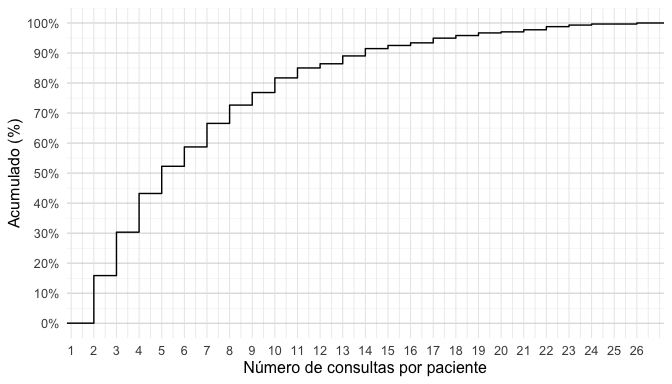
\includegraphics[width=1\textwidth,height=\textheight]{outputs/figs/n-consultas-ecdf-1.png}

}

\caption{Função de distribuição acumulada (ECDF) do número de consultas}

\end{figure}%

\begin{quote}
Legenda:\\
O gráfico ECDF mostra no eixo X o número de consultas por paciente e no
eixo Y a proporção acumulada de pacientes que atingiram até aquele
valor. Observa-se que cerca de \textbf{30\% dos pacientes tiveram até 3
consultas}, aproximadamente \textbf{50\% até 5 consultas (mediana)}, e
\textbf{75\% até 9 consultas (percentil 75)}. A curva se aproxima de
100\% em torno de 26 consultas, que é o valor máximo observado. Esse
tipo de gráfico facilita a visualização dos \textbf{percentis}: basta
projetar horizontalmente a linha desejada (25\%, 50\%, 75\%, etc.) até
interceptar a curva e ler no eixo X o valor correspondente de consultas.
\end{quote}

\begin{Shaded}
\begin{Highlighting}[]
\FunctionTok{library}\NormalTok{(dplyr)}
\FunctionTok{library}\NormalTok{(knitr)}

\NormalTok{resumo\_tempo\_seguimento }\OtherTok{\textless{}{-}}\NormalTok{ indicadores\_atendimento }\SpecialCharTok{\%\textgreater{}\%}
  \FunctionTok{summarise}\NormalTok{(}
    \AttributeTok{dias\_mediana    =} \FunctionTok{median}\NormalTok{(tempo\_seguimento\_dias, }\AttributeTok{na.rm =} \ConstantTok{TRUE}\NormalTok{),}
    \AttributeTok{dias\_IQR        =} \FunctionTok{IQR}\NormalTok{(tempo\_seguimento\_dias, }\AttributeTok{na.rm =} \ConstantTok{TRUE}\NormalTok{),}
    \AttributeTok{dias\_max        =} \FunctionTok{max}\NormalTok{(tempo\_seguimento\_dias, }\AttributeTok{na.rm =} \ConstantTok{TRUE}\NormalTok{),}
    
    \AttributeTok{semanas\_mediana =} \FunctionTok{median}\NormalTok{(tempo\_seguimento\_semanas, }\AttributeTok{na.rm =} \ConstantTok{TRUE}\NormalTok{),}
    \AttributeTok{semanas\_IQR     =} \FunctionTok{IQR}\NormalTok{(tempo\_seguimento\_semanas, }\AttributeTok{na.rm =} \ConstantTok{TRUE}\NormalTok{),}
    \AttributeTok{semanas\_max     =} \FunctionTok{max}\NormalTok{(tempo\_seguimento\_semanas, }\AttributeTok{na.rm =} \ConstantTok{TRUE}\NormalTok{),}
    
    \AttributeTok{meses\_mediana   =} \FunctionTok{median}\NormalTok{(tempo\_seguimento\_meses, }\AttributeTok{na.rm =} \ConstantTok{TRUE}\NormalTok{),}
    \AttributeTok{meses\_IQR       =} \FunctionTok{IQR}\NormalTok{(tempo\_seguimento\_meses, }\AttributeTok{na.rm =} \ConstantTok{TRUE}\NormalTok{),}
    \AttributeTok{meses\_max       =} \FunctionTok{max}\NormalTok{(tempo\_seguimento\_meses, }\AttributeTok{na.rm =} \ConstantTok{TRUE}\NormalTok{),}
    
    \AttributeTok{anos\_mediana    =} \FunctionTok{median}\NormalTok{(tempo\_seguimento\_anos, }\AttributeTok{na.rm =} \ConstantTok{TRUE}\NormalTok{),}
    \AttributeTok{anos\_IQR        =} \FunctionTok{IQR}\NormalTok{(tempo\_seguimento\_anos, }\AttributeTok{na.rm =} \ConstantTok{TRUE}\NormalTok{),}
    \AttributeTok{anos\_max        =} \FunctionTok{max}\NormalTok{(tempo\_seguimento\_anos, }\AttributeTok{na.rm =} \ConstantTok{TRUE}\NormalTok{)}
\NormalTok{  ) }\SpecialCharTok{\%\textgreater{}\%}
\NormalTok{  tidyr}\SpecialCharTok{::}\FunctionTok{pivot\_longer}\NormalTok{(}
    \AttributeTok{cols =} \FunctionTok{everything}\NormalTok{(),}
    \AttributeTok{names\_to =} \FunctionTok{c}\NormalTok{(}\StringTok{"tempo"}\NormalTok{, }\StringTok{"estatistica"}\NormalTok{),}
    \AttributeTok{names\_sep =} \StringTok{"\_"}\NormalTok{,}
    \AttributeTok{values\_to =} \StringTok{"valor"}
\NormalTok{  ) }\SpecialCharTok{\%\textgreater{}\%}
\NormalTok{  tidyr}\SpecialCharTok{::}\FunctionTok{pivot\_wider}\NormalTok{(}
    \AttributeTok{names\_from =}\NormalTok{ estatistica,}
    \AttributeTok{values\_from =}\NormalTok{ valor}
\NormalTok{  ) }\SpecialCharTok{\%\textgreater{}\%}
  \CommentTok{\# aplicar a função fmt com 2 casas decimais}
  \FunctionTok{mutate}\NormalTok{(}\FunctionTok{across}\NormalTok{(}\FunctionTok{c}\NormalTok{(mediana, IQR, max), }\SpecialCharTok{\textasciitilde{}}\FunctionTok{fmt}\NormalTok{(.x, }\AttributeTok{dec =} \DecValTok{1}\NormalTok{)))}

\FunctionTok{kable}\NormalTok{(resumo\_tempo\_seguimento,}
      \AttributeTok{caption =} \StringTok{"Tempo de seguimento em dias, semanas, meses e anos (mediana, IQR, máximo)"}\NormalTok{)}
\end{Highlighting}
\end{Shaded}

\begin{longtable}[]{@{}llll@{}}
\caption{Tempo de seguimento em dias, semanas, meses e anos (mediana,
IQR, máximo)}\tabularnewline
\toprule\noalign{}
tempo & mediana & IQR & max \\
\midrule\noalign{}
\endfirsthead
\toprule\noalign{}
tempo & mediana & IQR & max \\
\midrule\noalign{}
\endhead
\bottomrule\noalign{}
\endlastfoot
dias & 563,5 & 971,2 & 2.800,0 \\
semanas & 80,5 & 138,8 & 400,0 \\
meses & 18,5 & 31,9 & 92,0 \\
anos & 1,5 & 2,7 & 7,7 \\
\end{longtable}

Este código gera um resumo estatístico do tempo de seguimento dos
pacientes. Ele calcula, em diferentes unidades de tempo (dias, semanas,
meses e anos), a mediana, o intervalo interquartílico (IQR) e o valor
máximo do período entre a primeira e a última consulta. Em seguida,
reorganiza os resultados em formato de tabela longa e depois larga,
aplica formatação numérica com uma casa decimal, e apresenta a tabela
final com kable, facilitando a interpretação dos dados de seguimento.

\begin{Shaded}
\begin{Highlighting}[]
\CommentTok{\# Tabela com as estatísticas dos TEMPOS MÉDIOS entre consultas}
\NormalTok{resumo\_intervalos\_consultas }\OtherTok{\textless{}{-}}\NormalTok{ indicadores\_atendimento }\SpecialCharTok{\%\textgreater{}\%}
  \FunctionTok{summarise}\NormalTok{(}
    \AttributeTok{dias\_mediana    =} \FunctionTok{median}\NormalTok{(tempo\_medio\_entre\_consultas\_dias, }\AttributeTok{na.rm =} \ConstantTok{TRUE}\NormalTok{),}
    \AttributeTok{dias\_IQR        =} \FunctionTok{IQR}\NormalTok{(tempo\_medio\_entre\_consultas\_dias, }\AttributeTok{na.rm =} \ConstantTok{TRUE}\NormalTok{),}
    \AttributeTok{dias\_max        =} \FunctionTok{max}\NormalTok{(tempo\_medio\_entre\_consultas\_dias, }\AttributeTok{na.rm =} \ConstantTok{TRUE}\NormalTok{),}

    \AttributeTok{semanas\_mediana =} \FunctionTok{median}\NormalTok{(tempo\_medio\_entre\_consultas\_semanas, }\AttributeTok{na.rm =} \ConstantTok{TRUE}\NormalTok{),}
    \AttributeTok{semanas\_IQR     =} \FunctionTok{IQR}\NormalTok{(tempo\_medio\_entre\_consultas\_semanas, }\AttributeTok{na.rm =} \ConstantTok{TRUE}\NormalTok{),}
    \AttributeTok{semanas\_max     =} \FunctionTok{max}\NormalTok{(tempo\_medio\_entre\_consultas\_semanas, }\AttributeTok{na.rm =} \ConstantTok{TRUE}\NormalTok{),}

    \AttributeTok{meses\_mediana   =} \FunctionTok{median}\NormalTok{(tempo\_medio\_entre\_consultas\_meses, }\AttributeTok{na.rm =} \ConstantTok{TRUE}\NormalTok{),}
    \AttributeTok{meses\_IQR       =} \FunctionTok{IQR}\NormalTok{(tempo\_medio\_entre\_consultas\_meses, }\AttributeTok{na.rm =} \ConstantTok{TRUE}\NormalTok{),}
    \AttributeTok{meses\_max       =} \FunctionTok{max}\NormalTok{(tempo\_medio\_entre\_consultas\_meses, }\AttributeTok{na.rm =} \ConstantTok{TRUE}\NormalTok{),}

    \AttributeTok{anos\_mediana    =} \FunctionTok{median}\NormalTok{(tempo\_medio\_entre\_consultas\_anos, }\AttributeTok{na.rm =} \ConstantTok{TRUE}\NormalTok{),}
    \AttributeTok{anos\_IQR        =} \FunctionTok{IQR}\NormalTok{(tempo\_medio\_entre\_consultas\_anos, }\AttributeTok{na.rm =} \ConstantTok{TRUE}\NormalTok{),}
    \AttributeTok{anos\_max        =} \FunctionTok{max}\NormalTok{(tempo\_medio\_entre\_consultas\_anos, }\AttributeTok{na.rm =} \ConstantTok{TRUE}\NormalTok{)}
\NormalTok{  ) }\SpecialCharTok{\%\textgreater{}\%}
  \FunctionTok{pivot\_longer}\NormalTok{(}
    \AttributeTok{cols =} \FunctionTok{everything}\NormalTok{(),}
    \AttributeTok{names\_to =} \FunctionTok{c}\NormalTok{(}\StringTok{"tempo"}\NormalTok{, }\StringTok{"estatistica"}\NormalTok{),}
    \AttributeTok{names\_sep =} \StringTok{"\_"}\NormalTok{,}
    \AttributeTok{values\_to =} \StringTok{"valor"}
\NormalTok{  ) }\SpecialCharTok{\%\textgreater{}\%}
  \FunctionTok{pivot\_wider}\NormalTok{(}
    \AttributeTok{names\_from =}\NormalTok{ estatistica,}
    \AttributeTok{values\_from =}\NormalTok{ valor}
\NormalTok{  ) }\SpecialCharTok{\%\textgreater{}\%}
  \CommentTok{\# formatação com vírgula e 2 casas decimais usando sua função \textasciigrave{}fmt\textasciigrave{}}
  \FunctionTok{mutate}\NormalTok{(}\FunctionTok{across}\NormalTok{(}\FunctionTok{c}\NormalTok{(mediana, IQR, max), }\SpecialCharTok{\textasciitilde{}} \FunctionTok{fmt}\NormalTok{(.x, }\AttributeTok{dec =} \DecValTok{2}\NormalTok{)))}

\FunctionTok{kable}\NormalTok{(}
\NormalTok{  resumo\_intervalos\_consultas,}
  \AttributeTok{caption =} \StringTok{"Tempo médio entre consultas em dias, semanas, meses e anos (mediana, IQR, máximo)"}
\NormalTok{)}
\end{Highlighting}
\end{Shaded}

\begin{longtable}[]{@{}llll@{}}
\caption{Tempo médio entre consultas em dias, semanas, meses e anos
(mediana, IQR, máximo)}\tabularnewline
\toprule\noalign{}
tempo & mediana & IQR & max \\
\midrule\noalign{}
\endfirsthead
\toprule\noalign{}
tempo & mediana & IQR & max \\
\midrule\noalign{}
\endhead
\bottomrule\noalign{}
\endlastfoot
dias & 120,68 & 68,78 & 777,00 \\
semanas & 17,24 & 9,82 & 111,00 \\
meses & 3,96 & 2,26 & 25,53 \\
anos & 0,33 & 0,19 & 2,13 \\
\end{longtable}

Este código resume o tempo médio entre consultas dos pacientes. Ele
calcula, em dias, semanas, meses e anos, as medidas de posição e
dispersão: mediana, intervalo interquartílico (IQR) e valor máximo.
Depois, reorganiza os resultados em formato de tabela, aplica a
formatação numérica com duas casas decimais e apresenta a saída final de
forma organizada com kable, permitindo visualizar claramente os
intervalos médios entre as consultas.

\begin{quote}
Resultado: O tempo de seguimento dos pacientes apresentou grande
amplitude, variando de algumas semanas a mais de 7 anos. A mediana foi
de \textbf{18,5 meses} (IQR: 31,9), equivalente a \textbf{1,5 anos}
(IQR: 2,7), com máximo de \textbf{7,7 anos} de acompanhamento. Esse
resultado indica que metade dos pacientes foi acompanhada por até um ano
e meio, enquanto uma parcela menor permaneceu em seguimento prolongado
por vários anos.\\
O intervalo médio entre consultas também variou substancialmente. A
mediana foi de aproximadamente \textbf{120 dias} (IQR: 68,8), o que
corresponde a cerca de \textbf{4 meses} entre atendimentos. O percentil
superior mostra que alguns pacientes chegaram a intervalos médios de até
\textbf{777 dias} (mais de 2 anos) entre consultas, sugerindo padrões
heterogêneos de acompanhamento.\\
Em conjunto, esses achados mostram que a maioria dos pacientes foi
acompanhada em intervalos regulares de poucos meses, porém com
expressiva variação tanto na duração total do seguimento quanto na
frequência dos atendimentos.
\end{quote}

\begin{quote}
Resultado (versão curta): O tempo de seguimento variou amplamente, com
mediana de 1,5 anos e máximo de 7,7 anos. O intervalo médio entre
consultas foi de aproximadamente 4 meses (mediana: 120 dias), mas com
grande heterogeneidade entre os pacientes. O gráfico de dispersão mostra
que, embora a maioria mantenha retornos regulares em intervalos de até 6
meses, em seguimentos mais longos surgem casos com espaçamento
progressivamente maior entre consultas, alcançando mais de um ano.
\end{quote}

\begin{quote}
Discussão: Os achados referentes ao tempo de seguimento e ao intervalo
médio entre consultas sugerem um padrão heterogêneo de acompanhamento. A
maioria dos pacientes manteve retornos em intervalos regulares de 3 a 6
meses, consistentes com a prática clínica de monitoramento contínuo em
programas de tratamento da obesidade. Entretanto, nos casos de
seguimento mais longo observou-se um aumento progressivo na
variabilidade, incluindo pacientes com intervalos superiores a 12 meses
entre consultas. Esse comportamento pode refletir múltiplos fatores:
melhora clínica inicial que reduziu a necessidade de acompanhamento
frequente; dificuldades logísticas de comparecimento, como barreiras de
acesso e disponibilidade de serviços; ou ainda abandono parcial do
acompanhamento formal, com manutenção apenas de retornos ocasionais.\\
A presença desses dois perfis distintos --- pacientes com consultas
regulares e outros com retornos esparsos ao longo do tempo --- tem
implicações metodológicas e clínicas. Do ponto de vista analítico,
sugere cautela na interpretação das trajetórias de peso, já que o
espaçamento desigual pode introduzir vieses na avaliação da evolução
longitudinal. Do ponto de vista clínico, evidencia a importância de
estratégias que promovam maior adesão ao acompanhamento, sobretudo em
seguimentos prolongados, para garantir a continuidade do cuidado e a
detecção precoce de complicações associadas à obesidade.
\end{quote}

\begin{Shaded}
\begin{Highlighting}[]
\FunctionTok{library}\NormalTok{(ggplot2)}

\FunctionTok{ggplot}\NormalTok{(indicadores\_atendimento,}
       \FunctionTok{aes}\NormalTok{(}\AttributeTok{x =}\NormalTok{ tempo\_seguimento\_anos,}
           \AttributeTok{y =}\NormalTok{ tempo\_medio\_entre\_consultas\_meses)) }\SpecialCharTok{+}
  \FunctionTok{geom\_point}\NormalTok{(}\AttributeTok{alpha =} \FloatTok{0.5}\NormalTok{) }\SpecialCharTok{+}
  \FunctionTok{geom\_smooth}\NormalTok{(}\AttributeTok{method =} \StringTok{"lm"}\NormalTok{, }\AttributeTok{se =} \ConstantTok{TRUE}\NormalTok{, }\AttributeTok{color =} \StringTok{"blue"}\NormalTok{, }\AttributeTok{linewidth =} \FloatTok{0.8}\NormalTok{) }\SpecialCharTok{+}
  \FunctionTok{scale\_x\_continuous}\NormalTok{(}\AttributeTok{breaks =} \FunctionTok{seq}\NormalTok{(}\DecValTok{0}\NormalTok{, }\FunctionTok{max}\NormalTok{(indicadores\_atendimento}\SpecialCharTok{$}\NormalTok{tempo\_seguimento\_anos, }\AttributeTok{na.rm =} \ConstantTok{TRUE}\NormalTok{), }\AttributeTok{by =} \DecValTok{1}\NormalTok{)) }\SpecialCharTok{+}
  \FunctionTok{scale\_y\_continuous}\NormalTok{(}\AttributeTok{breaks =} \FunctionTok{seq}\NormalTok{(}\DecValTok{0}\NormalTok{, }\FunctionTok{max}\NormalTok{(indicadores\_atendimento}\SpecialCharTok{$}\NormalTok{tempo\_medio\_entre\_consultas\_meses, }\AttributeTok{na.rm =} \ConstantTok{TRUE}\NormalTok{), }\AttributeTok{by =} \DecValTok{2}\NormalTok{)) }\SpecialCharTok{+}
  \FunctionTok{labs}\NormalTok{(}
    \AttributeTok{x =} \StringTok{"Tempo de seguimento (anos)"}\NormalTok{,}
    \AttributeTok{y =} \StringTok{"Tempo médio entre consultas (meses)"}
\NormalTok{  ) }\SpecialCharTok{+}
  \FunctionTok{theme\_minimal}\NormalTok{(}\AttributeTok{base\_size =} \DecValTok{12}\NormalTok{)}
\end{Highlighting}
\end{Shaded}

\begin{verbatim}
`geom_smooth()` using formula = 'y ~ x'
\end{verbatim}

\begin{figure}[H]

{\centering 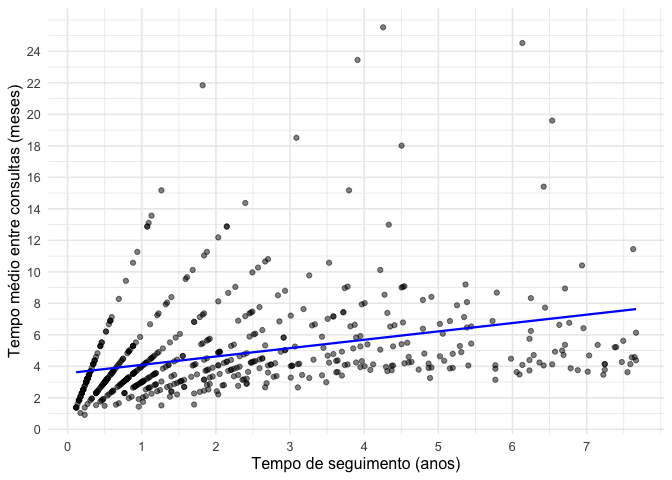
\includegraphics[width=1\textwidth,height=\textheight]{outputs/figs/seguimento-vs-intervalo-1.png}

}

\caption{Relação entre tempo total de seguimento e intervalo médio entre
consultas}

\end{figure}%

Este código gera um gráfico de dispersão para explorar a relação entre o
tempo total de seguimento dos pacientes (em anos) e o intervalo médio
entre consultas (em meses). Cada ponto representa um paciente, com
transparência aplicada para reduzir sobreposição. Além disso, é ajustada
uma linha de regressão linear com intervalo de confiança, destacada em
azul, para indicar a tendência da associação entre as duas variáveis. Os
eixos são configurados com quebras regulares para facilitar a leitura, e
a apresentação utiliza o tema minimalista para manter o gráfico limpo e
claro.

\begin{quote}
Legenda Figura X. Relação entre o tempo total de seguimento (anos) e o
intervalo médio entre consultas (meses). Cada ponto representa um
paciente; a linha azul indica a tendência linear. Observa-se que, embora
a maioria mantenha intervalos regulares de até 6 meses, em seguimentos
prolongados surgem casos com retornos mais espaçados, chegando a mais de
um ano. O gráfico de dispersão mostra a relação entre o \textbf{tempo
total de seguimento} (eixo X, em anos) e o \textbf{intervalo médio entre
consultas} (eixo Y, em meses) para cada paciente. Cada ponto representa
um indivíduo, e a linha azul corresponde à tendência linear ajustada.
\end{quote}

Observa-se que a maioria dos pacientes apresenta \textbf{intervalos
médios entre consultas de 2 a 6 meses}, independentemente da duração
total do seguimento. Contudo, conforme o tempo de acompanhamento
aumenta, surgem pacientes com intervalos progressivamente maiores,
alguns ultrapassando \textbf{12 meses} e chegando a mais de \textbf{20
meses} entre consultas em média. Isso explica a discreta inclinação
positiva da linha de tendência: em média, pacientes com seguimento mais
longo tendem a apresentar \textbf{consultas mais espaçadas}.

O padrão sugere dois grupos distintos:\\
1. \textbf{Seguimento curto a intermediário (até 2 anos)} ---
caracterizado por alta densidade de pontos e intervalos médios
regulares, geralmente abaixo de 6 meses.\\
2. \textbf{Seguimento prolongado (acima de 3--4 anos)} --- inclui
pacientes com \textbf{intervalos heterogêneos}, variando de intervalo de
seguimento regular até casos com retornos muito espaçados (\textgreater1
ano).

Esse achado reforça que, embora a mediana global seja de aproximadamente
\textbf{4 meses entre consultas}, há \textbf{grande heterogeneidade
individual}, especialmente entre pacientes mantidos em seguimento por
períodos mais longos.

\begin{Shaded}
\begin{Highlighting}[]
\FunctionTok{rm}\NormalTok{(}
  \CommentTok{\#indicadores\_atendimento,}
\NormalTok{  sumario\_n\_consultas,}
\NormalTok{  tabela\_frequencias,}
\NormalTok{  resumo\_tempo\_seguimento,}
\NormalTok{  resumo\_intervalos\_consultas}
\NormalTok{)}
\end{Highlighting}
\end{Shaded}

Limpa apenas os objetos intermediários criados durante a análise do item
1.3

\subsubsection{1.6. Proporção de indivíduos com peso final maior que o
inicial.}\label{proporuxe7uxe3o-de-indivuxedduos-com-peso-final-maior-que-o-inicial.}

\begin{Shaded}
\begin{Highlighting}[]
\CommentTok{\# Selecionar primeiro e último peso por paciente}
\NormalTok{peso\_inicial\_final }\OtherTok{\textless{}{-}}\NormalTok{ obese }\SpecialCharTok{\%\textgreater{}\%}
  \FunctionTok{group\_by}\NormalTok{(record\_id) }\SpecialCharTok{\%\textgreater{}\%}
  \FunctionTok{summarise}\NormalTok{(}
    \AttributeTok{peso\_inicial =} \FunctionTok{first}\NormalTok{(weight\_kg[}\FunctionTok{order}\NormalTok{(date\_consultation)]),}
    \AttributeTok{peso\_final   =} \FunctionTok{last}\NormalTok{(weight\_kg[}\FunctionTok{order}\NormalTok{(date\_consultation)]),}
    \AttributeTok{.groups =} \StringTok{"drop"}
\NormalTok{  ) }\SpecialCharTok{\%\textgreater{}\%}
  \FunctionTok{mutate}\NormalTok{(}\AttributeTok{ganhou\_peso =}\NormalTok{ peso\_final }\SpecialCharTok{\textgreater{}}\NormalTok{ peso\_inicial)}

\CommentTok{\# Calcular proporção e IC95\%}
\NormalTok{resultado\_peso\_final }\OtherTok{\textless{}{-}}\NormalTok{ peso\_inicial\_final }\SpecialCharTok{\%\textgreater{}\%}
  \FunctionTok{summarise}\NormalTok{(}
    \AttributeTok{n\_total =} \FunctionTok{n}\NormalTok{(),}
    \AttributeTok{n\_ganho =} \FunctionTok{sum}\NormalTok{(ganhou\_peso, }\AttributeTok{na.rm =} \ConstantTok{TRUE}\NormalTok{),}
    \AttributeTok{prop\_ganho =}\NormalTok{ n\_ganho }\SpecialCharTok{/}\NormalTok{ n\_total}
\NormalTok{  ) }\SpecialCharTok{\%\textgreater{}\%}
  \FunctionTok{mutate}\NormalTok{(}
    \AttributeTok{ic95 =} \FunctionTok{list}\NormalTok{(}\FunctionTok{binom.test}\NormalTok{(n\_ganho, n\_total)}\SpecialCharTok{$}\NormalTok{conf.int)}
\NormalTok{  ) }\SpecialCharTok{\%\textgreater{}\%}
  \FunctionTok{unnest\_wider}\NormalTok{(ic95, }\AttributeTok{names\_sep =} \StringTok{"\_"}\NormalTok{)}

\NormalTok{resultado\_peso\_final}
\end{Highlighting}
\end{Shaded}

\begin{verbatim}
# A tibble: 1 x 5
  n_total n_ganho prop_ganho ic95_1 ic95_2
    <int>   <int>      <dbl>  <dbl>  <dbl>
1     574     153      0.267  0.231  0.305
\end{verbatim}

Esse código seleciona o primeiro e o último peso de cada paciente,
compara-os e gera uma variável booleana (ganhou\_peso), que assume valor
1 (TRUE) quando o peso da última consulta foi maior que o peso da
primeira consulta. Em seguida, calcula-se a proporção de indivíduos cujo
peso final foi maior que o inicial, incluindo o intervalo de confiança
de 95\% (IC95\%) pelo teste binomial exato. O resultado mostra o número
total de pacientes avaliados, quantos ganharam peso no período e a
proporção correspondente, acompanhada do IC95\%.

\begin{quote}
Resultado:\\
Entre os \emph{574} indivíduos acompanhados, \textbf{153 (26,7\%;
IC95\%: 23,1--30,5\%) apresentaram peso final maior do que o peso
inicial}. Isso indica que aproximadamente um quarto dos pacientes teve
ganho ponderal ao longo do período de seguimento, enquanto a maioria
(73.3\%) apresentou peso final igual ou inferior ao inicial.\\
\end{quote}

\begin{quote}
Discussão:\\
Do ponto de vista clínico, esse achado sugere que, embora a maior parte
dos pacientes tenha conseguido manter ou reduzir o peso em relação ao
início do acompanhamento, ainda existe uma proporção considerável que
apresentou reganho ponderal. Esse fenômeno é consistente com a
literatura, que aponta a dificuldade de manutenção da perda de peso em
longo prazo, especialmente em contextos de obesidade, e reforça a
importância de estratégias de acompanhamento contínuo e intervenções
sustentadas para prevenção do reganho.
\end{quote}

\subsubsection{1.7. Proporção de consultas (a partir da segunda) com
ganho ou perda de peso em relação à
anterior/baseline.}\label{proporuxe7uxe3o-de-consultas-a-partir-da-segunda-com-ganho-ou-perda-de-peso-em-relauxe7uxe3o-uxe0-anteriorbaseline.}

Faremos duas análises para responder a perguntas diferentes:

\begin{enumerate}
\def\labelenumi{\arabic{enumi}.}
\tightlist
\item
  \textbf{Em relação à consulta anterior}

  \begin{itemize}
  \tightlist
  \item
    Mostra a \textbf{trajetória passo a passo}, ou seja, se o paciente
    está ganhando ou perdendo peso a cada intervalo entre consultas.\\
  \item
    Interessante para avaliar \textbf{flutuações} e estabilidade do peso
    ao longo do seguimento.\\
  \item
    Mais sensível a pequenas variações (até ruído de medida).
  \end{itemize}
\item
  \textbf{Em relação à primeira consulta}

  \begin{itemize}
  \tightlist
  \item
    Mostra a \textbf{tendência acumulada} desde o início do
    acompanhamento.\\
  \item
    Interessante para avaliar \textbf{manutenção de perda/ganho} ou se
    houve reversão em algum ponto.\\
  \item
    Mais robusto e fácil de interpretar em termos clínicos (baseline
    como referência).
  \end{itemize}
\end{enumerate}

Em geral, se o objetivo é \textbf{descrever a dinâmica do
acompanhamento}, a comparação com a \textbf{consulta anterior} (\#1)
costuma ser mais informativa, pois mostra o comportamento longitudinal.
Mas se o foco for \textbf{avaliar o impacto do acompanhamento em relação
ao estado inicial}, a comparação com a \textbf{primeira consulta} (\#2)
é mais clara e útil para comunicar resultados.

\textbf{Como interpretar e escolher o que reportar:}\\
- \textbf{Versus consulta anterior:} útil para descrever a
\textbf{dinâmica entre visitas}, sensível a flutuações; ideal para
``trajetória'' do cuidado.\\
- \textbf{Versus baseline:} comunica a \textbf{tendência acumulada}
desde o início; costuma ser mais estável e clinicamente intuitiva.

Se o artigo tiver espaço, recomendo \textbf{reportar ambos} (principal =
baseline; secundário = anterior), pois oferecem perspectivas
complementares. Caso precise enxugar, priorize a definição que melhor se
alinha ao objetivo do capítulo: \textbf{efeito do seguimento} (baseline)
vs \textbf{padrão de flutuação} (anterior).

\begin{Shaded}
\begin{Highlighting}[]
\CommentTok{\# Preparação: função auxiliar de IC95\% para proporção}

\NormalTok{ci\_prop }\OtherTok{\textless{}{-}} \ControlFlowTok{function}\NormalTok{(x, n, }\AttributeTok{conf.level =} \FloatTok{0.95}\NormalTok{) \{}
  \CommentTok{\# x = sucessos; n = total}
  \ControlFlowTok{if}\NormalTok{ (}\FunctionTok{is.na}\NormalTok{(x) }\SpecialCharTok{||} \FunctionTok{is.na}\NormalTok{(n) }\SpecialCharTok{||}\NormalTok{ n }\SpecialCharTok{==} \DecValTok{0}\NormalTok{) \{}
    \FunctionTok{return}\NormalTok{(}\FunctionTok{tibble}\NormalTok{(}\AttributeTok{prop =} \ConstantTok{NA\_real\_}\NormalTok{, }\AttributeTok{lcl =} \ConstantTok{NA\_real\_}\NormalTok{, }\AttributeTok{ucl =} \ConstantTok{NA\_real\_}\NormalTok{))}
\NormalTok{  \}}
\NormalTok{  pt }\OtherTok{\textless{}{-}}\NormalTok{ stats}\SpecialCharTok{::}\FunctionTok{prop.test}\NormalTok{(}\AttributeTok{x =}\NormalTok{ x, }\AttributeTok{n =}\NormalTok{ n, }\AttributeTok{conf.level =}\NormalTok{ conf.level, }\AttributeTok{correct =} \ConstantTok{FALSE}\NormalTok{)}
  \FunctionTok{tibble}\NormalTok{(}
    \AttributeTok{prop =} \FunctionTok{unname}\NormalTok{(pt}\SpecialCharTok{$}\NormalTok{estimate),}
    \AttributeTok{lcl  =} \FunctionTok{unname}\NormalTok{(pt}\SpecialCharTok{$}\NormalTok{conf.int[}\DecValTok{1}\NormalTok{]),}
    \AttributeTok{ucl  =} \FunctionTok{unname}\NormalTok{(pt}\SpecialCharTok{$}\NormalTok{conf.int[}\DecValTok{2}\NormalTok{])}
\NormalTok{  )}
\NormalTok{\}}
\end{Highlighting}
\end{Shaded}

Este chunk define \texttt{ci\_prop()}, que calcula proporções com IC95\%
(teste de proporções com correção de continuidade desabilitada,
aproximando o intervalo de Wilson).

\begin{Shaded}
\begin{Highlighting}[]
\CommentTok{\# 1) Ordenar consultas dentro de cada paciente}
\CommentTok{\# 2) Criar deltas e direções vs consulta anterior e vs baseline}
\CommentTok{\# 3) Manter apenas consultas a partir da 2ª, com peso observado}

\NormalTok{obese\_ord }\OtherTok{\textless{}{-}}\NormalTok{ obese }\SpecialCharTok{\%\textgreater{}\%}
  \FunctionTok{arrange}\NormalTok{(record\_id, index, date\_consultation) }\SpecialCharTok{\%\textgreater{}\%}
  \FunctionTok{group\_by}\NormalTok{(record\_id) }\SpecialCharTok{\%\textgreater{}\%}
  \FunctionTok{mutate}\NormalTok{(}
    \CommentTok{\# vs consulta anterior}
    \AttributeTok{weight\_prev   =}\NormalTok{ dplyr}\SpecialCharTok{::}\FunctionTok{lag}\NormalTok{(weight\_kg),}
    \AttributeTok{delta\_prev\_kg =} \FunctionTok{if\_else}\NormalTok{(}\SpecialCharTok{!}\FunctionTok{is.na}\NormalTok{(weight\_kg) }\SpecialCharTok{\&} \SpecialCharTok{!}\FunctionTok{is.na}\NormalTok{(weight\_prev),}
\NormalTok{                            weight\_kg }\SpecialCharTok{{-}}\NormalTok{ weight\_prev, }\ConstantTok{NA\_real\_}\NormalTok{),}
    \AttributeTok{dir\_prev =} \FunctionTok{case\_when}\NormalTok{(}
      \FunctionTok{is.na}\NormalTok{(delta\_prev\_kg)         }\SpecialCharTok{\textasciitilde{}} \ConstantTok{NA\_character\_}\NormalTok{,}
\NormalTok{      delta\_prev\_kg }\SpecialCharTok{\textgreater{}} \DecValTok{0}            \SpecialCharTok{\textasciitilde{}} \StringTok{"ganho"}\NormalTok{,}
\NormalTok{      delta\_prev\_kg }\SpecialCharTok{\textless{}} \DecValTok{0}            \SpecialCharTok{\textasciitilde{}} \StringTok{"perda"}\NormalTok{,}
\NormalTok{      delta\_prev\_kg }\SpecialCharTok{==} \DecValTok{0}           \SpecialCharTok{\textasciitilde{}} \StringTok{"estável"}
\NormalTok{    ),}
    \CommentTok{\# vs baseline (utiliza baseline\_weight fornecido no dataset)}
    \AttributeTok{delta\_base\_kg =} \FunctionTok{if\_else}\NormalTok{(}\SpecialCharTok{!}\FunctionTok{is.na}\NormalTok{(weight\_kg) }\SpecialCharTok{\&} \SpecialCharTok{!}\FunctionTok{is.na}\NormalTok{(baseline\_weight),}
\NormalTok{                            weight\_kg }\SpecialCharTok{{-}}\NormalTok{ baseline\_weight, }\ConstantTok{NA\_real\_}\NormalTok{),}
    \AttributeTok{dir\_base =} \FunctionTok{case\_when}\NormalTok{(}
      \FunctionTok{is.na}\NormalTok{(delta\_base\_kg)         }\SpecialCharTok{\textasciitilde{}} \ConstantTok{NA\_character\_}\NormalTok{,}
\NormalTok{      delta\_base\_kg }\SpecialCharTok{\textgreater{}} \DecValTok{0}            \SpecialCharTok{\textasciitilde{}} \StringTok{"ganho"}\NormalTok{,}
\NormalTok{      delta\_base\_kg }\SpecialCharTok{\textless{}} \DecValTok{0}            \SpecialCharTok{\textasciitilde{}} \StringTok{"perda"}\NormalTok{,}
\NormalTok{      delta\_base\_kg }\SpecialCharTok{==} \DecValTok{0}           \SpecialCharTok{\textasciitilde{}} \StringTok{"estável"}
\NormalTok{    )}
\NormalTok{  ) }\SpecialCharTok{\%\textgreater{}\%}
  \FunctionTok{ungroup}\NormalTok{()}

\CommentTok{\# Elegibilidade: consultas a partir da segunda e com comparador válido}
\NormalTok{ eleg\_prev }\OtherTok{\textless{}{-}}\NormalTok{ obese\_ord }\SpecialCharTok{\%\textgreater{}\%}
  \FunctionTok{filter}\NormalTok{(index }\SpecialCharTok{\textgreater{}=} \DecValTok{2}\NormalTok{, }\SpecialCharTok{!}\FunctionTok{is.na}\NormalTok{(delta\_prev\_kg), }\SpecialCharTok{!}\FunctionTok{is.na}\NormalTok{(dir\_prev))}

\NormalTok{ eleg\_base }\OtherTok{\textless{}{-}}\NormalTok{ obese\_ord }\SpecialCharTok{\%\textgreater{}\%}
  \FunctionTok{filter}\NormalTok{(index }\SpecialCharTok{\textgreater{}=} \DecValTok{2}\NormalTok{, }\SpecialCharTok{!}\FunctionTok{is.na}\NormalTok{(delta\_base\_kg), }\SpecialCharTok{!}\FunctionTok{is.na}\NormalTok{(dir\_base))}
\end{Highlighting}
\end{Shaded}

Aqui organizamos o banco por paciente e consulta, criamos as diferenças
de peso em kg vs a consulta anterior e vs a baseline, rotulando cada
consulta (≥2ª) como ``ganho'', ``perda'' ou ``estável''. Geramos dois
subconjuntos elegíveis: \texttt{eleg\_prev} (comparação com a anterior)
e \texttt{eleg\_base} (comparação com a baseline).

\begin{Shaded}
\begin{Highlighting}[]
\CommentTok{\# Função para sumarizar proporções por direção (ganho/perda/estável)}
\CommentTok{\# Ela calcula os ICs com \textasciigrave{}ci\_prop()\textasciigrave{} e faz \textasciigrave{}bind\_cols()\textasciigrave{} de forma explícita.}

\NormalTok{sumarizar\_proporcoes }\OtherTok{\textless{}{-}} \ControlFlowTok{function}\NormalTok{(df, dir\_col) \{}
  \CommentTok{\# 1) Contagens básicas}
\NormalTok{  base }\OtherTok{\textless{}{-}}\NormalTok{ df }\SpecialCharTok{\%\textgreater{}\%}
    \FunctionTok{summarize}\NormalTok{(}
      \AttributeTok{total\_consultas =}\NormalTok{ dplyr}\SpecialCharTok{::}\FunctionTok{n}\NormalTok{(),}
      \AttributeTok{n\_ganho   =} \FunctionTok{sum}\NormalTok{(.data[[dir\_col]] }\SpecialCharTok{==} \StringTok{"ganho"}\NormalTok{,   }\AttributeTok{na.rm =} \ConstantTok{TRUE}\NormalTok{),}
      \AttributeTok{n\_perda   =} \FunctionTok{sum}\NormalTok{(.data[[dir\_col]] }\SpecialCharTok{==} \StringTok{"perda"}\NormalTok{,   }\AttributeTok{na.rm =} \ConstantTok{TRUE}\NormalTok{),}
      \AttributeTok{n\_estavel =} \FunctionTok{sum}\NormalTok{(.data[[dir\_col]] }\SpecialCharTok{==} \StringTok{"estável"}\NormalTok{, }\AttributeTok{na.rm =} \ConstantTok{TRUE}\NormalTok{)}
\NormalTok{    )}

  \CommentTok{\# 2) IC95\% por direção (devolve data.frames 1x3)}
\NormalTok{  ci\_g }\OtherTok{\textless{}{-}} \FunctionTok{ci\_prop}\NormalTok{(base}\SpecialCharTok{$}\NormalTok{n\_ganho,   base}\SpecialCharTok{$}\NormalTok{total\_consultas) }\SpecialCharTok{\%\textgreater{}\%}
\NormalTok{    dplyr}\SpecialCharTok{::}\FunctionTok{rename}\NormalTok{(}\AttributeTok{prop\_ganho =}\NormalTok{ prop, }\AttributeTok{lcl\_ganho =}\NormalTok{ lcl, }\AttributeTok{ucl\_ganho =}\NormalTok{ ucl)}

\NormalTok{  ci\_p }\OtherTok{\textless{}{-}} \FunctionTok{ci\_prop}\NormalTok{(base}\SpecialCharTok{$}\NormalTok{n\_perda,   base}\SpecialCharTok{$}\NormalTok{total\_consultas) }\SpecialCharTok{\%\textgreater{}\%}
\NormalTok{    dplyr}\SpecialCharTok{::}\FunctionTok{rename}\NormalTok{(}\AttributeTok{prop\_perda =}\NormalTok{ prop, }\AttributeTok{lcl\_perda =}\NormalTok{ lcl, }\AttributeTok{ucl\_perda =}\NormalTok{ ucl)}

\NormalTok{  ci\_e }\OtherTok{\textless{}{-}} \FunctionTok{ci\_prop}\NormalTok{(base}\SpecialCharTok{$}\NormalTok{n\_estavel, base}\SpecialCharTok{$}\NormalTok{total\_consultas) }\SpecialCharTok{\%\textgreater{}\%}
\NormalTok{    dplyr}\SpecialCharTok{::}\FunctionTok{rename}\NormalTok{(}\AttributeTok{prop\_estavel =}\NormalTok{ prop, }\AttributeTok{lcl\_estavel =}\NormalTok{ lcl, }\AttributeTok{ucl\_estavel =}\NormalTok{ ucl)}

  \CommentTok{\# 3) Juntar tudo de forma determinística}
\NormalTok{  out }\OtherTok{\textless{}{-}}\NormalTok{ dplyr}\SpecialCharTok{::}\FunctionTok{bind\_cols}\NormalTok{(base, ci\_g, ci\_p, ci\_e) }\SpecialCharTok{\%\textgreater{}\%}
\NormalTok{    dplyr}\SpecialCharTok{::}\FunctionTok{mutate}\NormalTok{(}
      \AttributeTok{prop\_ganho\_pct   =}\NormalTok{ scales}\SpecialCharTok{::}\FunctionTok{percent}\NormalTok{(prop\_ganho,   }\AttributeTok{accuracy =} \FloatTok{0.1}\NormalTok{),}
      \AttributeTok{prop\_perda\_pct   =}\NormalTok{ scales}\SpecialCharTok{::}\FunctionTok{percent}\NormalTok{(prop\_perda,   }\AttributeTok{accuracy =} \FloatTok{0.1}\NormalTok{),}
      \AttributeTok{prop\_estavel\_pct =}\NormalTok{ scales}\SpecialCharTok{::}\FunctionTok{percent}\NormalTok{(prop\_estavel, }\AttributeTok{accuracy =} \FloatTok{0.1}\NormalTok{),}
      \AttributeTok{ic\_ganho   =} \FunctionTok{sprintf}\NormalTok{(}\StringTok{"ganho (\%.1f\%\%; IC95\%\% \%.1f\%\%–\%.1f\%\%)"}\NormalTok{,}
                           \DecValTok{100}\SpecialCharTok{*}\NormalTok{prop\_ganho, }\DecValTok{100}\SpecialCharTok{*}\NormalTok{lcl\_ganho, }\DecValTok{100}\SpecialCharTok{*}\NormalTok{ucl\_ganho),}
      \AttributeTok{ic\_perda   =} \FunctionTok{sprintf}\NormalTok{(}\StringTok{"perda (\%.1f\%\%; IC95\%\% \%.1f\%\%–\%.1f\%\%)"}\NormalTok{,}
                           \DecValTok{100}\SpecialCharTok{*}\NormalTok{prop\_perda, }\DecValTok{100}\SpecialCharTok{*}\NormalTok{lcl\_perda, }\DecValTok{100}\SpecialCharTok{*}\NormalTok{ucl\_perda),}
      \AttributeTok{ic\_estavel =} \FunctionTok{sprintf}\NormalTok{(}\StringTok{"estável (\%.1f\%\%; IC95\%\% \%.1f\%\%–\%.1f\%\%)"}\NormalTok{,}
                           \DecValTok{100}\SpecialCharTok{*}\NormalTok{prop\_estavel, }\DecValTok{100}\SpecialCharTok{*}\NormalTok{lcl\_estavel, }\DecValTok{100}\SpecialCharTok{*}\NormalTok{ucl\_estavel)}
\NormalTok{    ) }\SpecialCharTok{\%\textgreater{}\%}
\NormalTok{    dplyr}\SpecialCharTok{::}\FunctionTok{select}\NormalTok{(}
\NormalTok{      total\_consultas,}
\NormalTok{      n\_ganho, n\_perda, n\_estavel,}
\NormalTok{      prop\_ganho\_pct, prop\_perda\_pct, prop\_estavel\_pct,}
\NormalTok{      ic\_ganho, ic\_perda, ic\_estavel}
\NormalTok{    )}

\NormalTok{  out}
\NormalTok{\}}

\CommentTok{\# 1) Proporções vs consulta anterior}
\NormalTok{res\_prev }\OtherTok{\textless{}{-}} \FunctionTok{sumarizar\_proporcoes}\NormalTok{(eleg\_prev, }\StringTok{"dir\_prev"}\NormalTok{)}

\CommentTok{\# 2) Proporções vs baseline}
\NormalTok{res\_base }\OtherTok{\textless{}{-}} \FunctionTok{sumarizar\_proporcoes}\NormalTok{(eleg\_base, }\StringTok{"dir\_base"}\NormalTok{)}

\NormalTok{res\_prev}
\end{Highlighting}
\end{Shaded}

\begin{verbatim}
# A tibble: 1 x 10
  total_consultas n_ganho n_perda n_estavel prop_ganho_pct prop_perda_pct
            <int>   <int>   <int>     <int> <chr>          <chr>         
1            2328    1026    1243        59 44.1%          53.4%         
# i 4 more variables: prop_estavel_pct <chr>, ic_ganho <chr>, ic_perda <chr>,
#   ic_estavel <chr>
\end{verbatim}

\begin{Shaded}
\begin{Highlighting}[]
\NormalTok{res\_base}
\end{Highlighting}
\end{Shaded}

\begin{verbatim}
# A tibble: 1 x 10
  total_consultas n_ganho n_perda n_estavel prop_ganho_pct prop_perda_pct
            <int>   <int>   <int>     <int> <chr>          <chr>         
1            2670     954    1594       122 35.7%          59.7%         
# i 4 more variables: prop_estavel_pct <chr>, ic_ganho <chr>, ic_perda <chr>,
#   ic_estavel <chr>
\end{verbatim}

Este chunk calcula, para todas as consultas elegíveis (≥2ª), as
proporções e IC95\% de ``ganho'', ``perda'' e ``estável'' sob duas
definições: 1. vs consulta anterior (res\_prev) --- dinâmica entre
visitas consecutivas; 2. vs baseline (res\_base) --- tendência acumulada
desde a primeira consulta.

As tabelas retornam o número total de consultas analisadas, contagens
por direção e as proporções com IC95\%.

\begin{Shaded}
\begin{Highlighting}[]
\CommentTok{\# Tabelas prontas para o artigo (formato longo e legível)}

\NormalTok{formatar\_tabela }\OtherTok{\textless{}{-}} \ControlFlowTok{function}\NormalTok{(tb, titulo) \{}
\NormalTok{  tibble}\SpecialCharTok{::}\FunctionTok{tibble}\NormalTok{(}
\NormalTok{    Definição }\OtherTok{=}\NormalTok{ titulo,}
    \StringTok{\textasciigrave{}}\AttributeTok{Consultas elegíveis (n)}\StringTok{\textasciigrave{}} \OtherTok{=}\NormalTok{ tb}\SpecialCharTok{$}\NormalTok{total\_consultas,}
    \StringTok{\textasciigrave{}}\AttributeTok{Ganho, n (\%) [IC95\%]}\StringTok{\textasciigrave{}}    \OtherTok{=} \FunctionTok{sprintf}\NormalTok{(}\StringTok{"\%d (\%s) — \%s"}\NormalTok{, tb}\SpecialCharTok{$}\NormalTok{n\_ganho, tb}\SpecialCharTok{$}\NormalTok{prop\_ganho\_pct, tb}\SpecialCharTok{$}\NormalTok{ic\_ganho),}
    \StringTok{\textasciigrave{}}\AttributeTok{Perda, n (\%) [IC95\%]}\StringTok{\textasciigrave{}}    \OtherTok{=} \FunctionTok{sprintf}\NormalTok{(}\StringTok{"\%d (\%s) — \%s"}\NormalTok{, tb}\SpecialCharTok{$}\NormalTok{n\_perda, tb}\SpecialCharTok{$}\NormalTok{prop\_perda\_pct, tb}\SpecialCharTok{$}\NormalTok{ic\_perda),}
    \StringTok{\textasciigrave{}}\AttributeTok{Estável, n (\%) [IC95\%]}\StringTok{\textasciigrave{}}  \OtherTok{=} \FunctionTok{sprintf}\NormalTok{(}\StringTok{"\%d (\%s) — \%s"}\NormalTok{, tb}\SpecialCharTok{$}\NormalTok{n\_estavel, tb}\SpecialCharTok{$}\NormalTok{prop\_estavel\_pct, tb}\SpecialCharTok{$}\NormalTok{ic\_estavel)}
\NormalTok{  )}
\NormalTok{\}}

\NormalTok{tab\_prev }\OtherTok{\textless{}{-}} \FunctionTok{formatar\_tabela}\NormalTok{(res\_prev, }\StringTok{"Em relação à consulta anterior"}\NormalTok{)}
\NormalTok{tab\_base }\OtherTok{\textless{}{-}} \FunctionTok{formatar\_tabela}\NormalTok{(res\_base, }\StringTok{"Em relação à primeira consulta (baseline)"}\NormalTok{)}

\NormalTok{knitr}\SpecialCharTok{::}\FunctionTok{kable}\NormalTok{(}
  \FunctionTok{rbind}\NormalTok{(tab\_prev, tab\_base),}
  \AttributeTok{caption =} \StringTok{"Proporção de consultas (a partir da segunda) com ganho, perda ou estabilidade de peso"}\NormalTok{,}
  \AttributeTok{align =} \FunctionTok{c}\NormalTok{(}\StringTok{"l"}\NormalTok{, }\StringTok{"r"}\NormalTok{, }\StringTok{"l"}\NormalTok{, }\StringTok{"l"}\NormalTok{, }\StringTok{"l"}\NormalTok{),}
  \AttributeTok{col.names =} \FunctionTok{c}\NormalTok{(}\StringTok{"Definição"}\NormalTok{, }\StringTok{"Consultas elegíveis (n)"}\NormalTok{, }\StringTok{"Ganho, n (\%) [IC95\%]"}\NormalTok{, }\StringTok{"Perda, n (\%) [IC95\%]"}\NormalTok{, }\StringTok{"Estável, n (\%) [IC95\%]"}\NormalTok{)}
\NormalTok{)}
\end{Highlighting}
\end{Shaded}

\begin{longtable}[]{@{}
  >{\raggedright\arraybackslash}p{(\columnwidth - 8\tabcolsep) * \real{0.2029}}
  >{\raggedleft\arraybackslash}p{(\columnwidth - 8\tabcolsep) * \real{0.1159}}
  >{\raggedright\arraybackslash}p{(\columnwidth - 8\tabcolsep) * \real{0.2319}}
  >{\raggedright\arraybackslash}p{(\columnwidth - 8\tabcolsep) * \real{0.2319}}
  >{\raggedright\arraybackslash}p{(\columnwidth - 8\tabcolsep) * \real{0.2174}}@{}}
\caption{Proporção de consultas (a partir da segunda) com ganho, perda
ou estabilidade de peso}\tabularnewline
\toprule\noalign{}
\begin{minipage}[b]{\linewidth}\raggedright
Definição
\end{minipage} & \begin{minipage}[b]{\linewidth}\raggedleft
Consultas elegíveis (n)
\end{minipage} & \begin{minipage}[b]{\linewidth}\raggedright
Ganho, n (\%) {[}IC95\%{]}
\end{minipage} & \begin{minipage}[b]{\linewidth}\raggedright
Perda, n (\%) {[}IC95\%{]}
\end{minipage} & \begin{minipage}[b]{\linewidth}\raggedright
Estável, n (\%) {[}IC95\%{]}
\end{minipage} \\
\midrule\noalign{}
\endfirsthead
\toprule\noalign{}
\begin{minipage}[b]{\linewidth}\raggedright
Definição
\end{minipage} & \begin{minipage}[b]{\linewidth}\raggedleft
Consultas elegíveis (n)
\end{minipage} & \begin{minipage}[b]{\linewidth}\raggedright
Ganho, n (\%) {[}IC95\%{]}
\end{minipage} & \begin{minipage}[b]{\linewidth}\raggedright
Perda, n (\%) {[}IC95\%{]}
\end{minipage} & \begin{minipage}[b]{\linewidth}\raggedright
Estável, n (\%) {[}IC95\%{]}
\end{minipage} \\
\midrule\noalign{}
\endhead
\bottomrule\noalign{}
\endlastfoot
Em relação à consulta anterior & 2328 & 1026 (44.1\%) --- ganho (44.1\%;
IC95\% 42.1\%--46.1\%) & 1243 (53.4\%) --- perda (53.4\%; IC95\%
51.4\%--55.4\%) & 59 (2.5\%) --- estável (2.5\%; IC95\% 2.0\%--3.3\%) \\
Em relação à primeira consulta (baseline) & 2670 & 954 (35.7\%) ---
ganho (35.7\%; IC95\% 33.9\%--37.6\%) & 1594 (59.7\%) --- perda (59.7\%;
IC95\% 57.8\%--61.5\%) & 122 (4.6\%) --- estável (4.6\%; IC95\%
3.8\%--5.4\%) \\
\end{longtable}

Aqui formatamos duas tabelas finais, prontas para inserir no
relatório/artigo: uma em relação à consulta anterior e outra em relação
à baseline. Cada linha traz o total de consultas analisadas, a contagem
e a proporção (\%) com IC95\% para ``ganho'', ``perda'' e ``estável''.

\begin{quote}
Resultados:\\
Entre as consultas analisadas a partir da segunda visita, observou-se
que \textbf{44,1\% (IC95\% 42,1--46,1)} apresentaram ganho de peso em
relação à consulta imediatamente anterior, enquanto \textbf{53,4\%
(IC95\% 51,4--55,4)} mostraram perda de peso e \textbf{2,5\% (IC95\%
2,0--3,3)} permaneceram estáveis.\\
Quando a referência foi a primeira consulta (baseline), os resultados
evidenciaram uma tendência acumulada diferente: \textbf{35,7\% (IC95\%
33,9--37,6)} das consultas estavam associadas a ganho de peso em relação
ao basal, \textbf{59,7\% (IC95\% 57,8--61,5)} a perda de peso, e
\textbf{4,6\% (IC95\% 3,8--5,4)} mantiveram peso estável.\\
Portanto, embora a análise \textbf{visita a visita} revele flutuações
mais frequentes de ganho e perda, a comparação \textbf{com o peso
inicial} sugere que, no seguimento acumulado, predominou a perda de
peso.\\
\end{quote}

\begin{quote}
Discussão:\\
A análise longitudinal de perda de peso mostrou padrões distintos
conforme o critério de referência utilizado. Considerando-se a consulta
imediatamente anterior, a evolução do peso revelou \textbf{alta
variabilidade}, com proporções semelhantes de consultas com ganho e
perda, refletindo as oscilações individuais e possivelmente influências
transitórias de fatores comportamentais, clínicos ou mesmo variações
técnicas de medida.\\
Por outro lado, quando o peso inicial foi adotado como referência,
observou-se uma \textbf{tendência global de perda de peso} ao longo do
seguimento, evidenciada por maior proporção de consultas classificadas
como perda em relação ao basal. Este resultado sugere que, apesar das
flutuações entre visitas, o acompanhamento clínico contribuiu para um
saldo positivo na redução de peso em termos cumulativos.\\
A diferença entre os dois enfoques analíticos é relevante. A comparação
visita a visita é mais sensível a pequenas variações, que podem
representar tanto mudanças reais quanto ruído de mensuração. Já a
comparação acumulada com o peso basal tende a capturar melhor o efeito
do seguimento como um todo, sendo clinicamente mais intuitiva para
avaliar impacto do tratamento.\\
Do ponto de vista clínico, a predominância de perda de peso acumulada
sugere benefício do acompanhamento, mas a presença consistente de
oscilações reforça a necessidade de estratégias para manutenção do peso
e prevenção do reganho.
\end{quote}

\begin{Shaded}
\begin{Highlighting}[]
\CommentTok{\# (Opcional) Exemplo de estratificação por tempo de seguimento ou por sexo/etnia}
\CommentTok{\# Ajuste os "group\_by" conforme sua necessidade analítica.}

\CommentTok{\# Ex.: estratificar por sexo para a definição "vs consulta anterior"}
\CommentTok{\# Correção robusta para estratificar por SEXO.}
\CommentTok{\# Evita problemas de coluna ausente ou conflitos de nomes após o join.}
\CommentTok{\# Correção para o erro: “Can\textquotesingle{}t subset \textasciigrave{}.data\textasciigrave{} outside of a data mask context.”}
\CommentTok{\# Isso ocorre quando usamos \textasciigrave{}.data[[grp\_col]]\textasciigrave{} fora de verbos *data{-}masked* do dplyr}
\CommentTok{\# (ex.: dentro de \textasciigrave{}select()\textasciigrave{} ou \textasciigrave{}complete()\textasciigrave{} sem embrulhar com tidy evaluation).}
\CommentTok{\# Abaixo, reescrevo a função usando tidy evaluation com \textasciigrave{}\{ \}\textasciigrave{} e \textasciigrave{}all\_of()\textasciigrave{}.}

\FunctionTok{library}\NormalTok{(dplyr)}
\FunctionTok{library}\NormalTok{(tidyr)}
\FunctionTok{library}\NormalTok{(purrr)}
\FunctionTok{library}\NormalTok{(rlang)}

\CommentTok{\# Lookup "many{-}to{-}one" para sexo por paciente}
\NormalTok{lkp\_sex }\OtherTok{\textless{}{-}}\NormalTok{ obese }\SpecialCharTok{\%\textgreater{}\%}
  \FunctionTok{distinct}\NormalTok{(record\_id, sex) }\SpecialCharTok{\%\textgreater{}\%}
  \FunctionTok{rename}\NormalTok{(}\AttributeTok{sex\_lookup =}\NormalTok{ sex)}

\CommentTok{\# Função robusta: usa tidy evaluation para permitir \textasciigrave{}grp\_col\textasciigrave{} como string ou símbolo}
\NormalTok{sumarizar\_proporcoes\_grupo }\OtherTok{\textless{}{-}} \ControlFlowTok{function}\NormalTok{(df, dir\_col, grp\_col) \{}
  \CommentTok{\# capturar colunas como símbolos}
\NormalTok{  dir\_col }\OtherTok{\textless{}{-}} \FunctionTok{enquo}\NormalTok{(dir\_col)}
\NormalTok{  grp\_col }\OtherTok{\textless{}{-}} \FunctionTok{enquo}\NormalTok{(grp\_col)}

  \CommentTok{\# total por grupo}
\NormalTok{  tot }\OtherTok{\textless{}{-}}\NormalTok{ df }\SpecialCharTok{\%\textgreater{}\%}
    \FunctionTok{group\_by}\NormalTok{(}\SpecialCharTok{!!}\NormalTok{grp\_col) }\SpecialCharTok{\%\textgreater{}\%}
    \FunctionTok{summarize}\NormalTok{(}\AttributeTok{total\_consultas =} \FunctionTok{n}\NormalTok{(), }\AttributeTok{.groups =} \StringTok{"drop"}\NormalTok{)}

  \CommentTok{\# contagens por direção dentro de cada grupo}
\NormalTok{  cont }\OtherTok{\textless{}{-}}\NormalTok{ df }\SpecialCharTok{\%\textgreater{}\%}
    \FunctionTok{group\_by}\NormalTok{(}\SpecialCharTok{!!}\NormalTok{grp\_col, }\AttributeTok{direcao =} \SpecialCharTok{!!}\NormalTok{dir\_col) }\SpecialCharTok{\%\textgreater{}\%}
    \FunctionTok{summarize}\NormalTok{(}\AttributeTok{n =} \FunctionTok{n}\NormalTok{(), }\AttributeTok{.groups =} \StringTok{"drop"}\NormalTok{)}

  \CommentTok{\# garantir as três categorias em cada grupo}
\NormalTok{  base }\OtherTok{\textless{}{-}}\NormalTok{ cont }\SpecialCharTok{\%\textgreater{}\%}
\NormalTok{    tidyr}\SpecialCharTok{::}\FunctionTok{complete}\NormalTok{(}
      \SpecialCharTok{!!}\NormalTok{grp\_col,}
      \AttributeTok{direcao =} \FunctionTok{c}\NormalTok{(}\StringTok{"ganho"}\NormalTok{,}\StringTok{"perda"}\NormalTok{,}\StringTok{"estável"}\NormalTok{),}
      \AttributeTok{fill =} \FunctionTok{list}\NormalTok{(}\AttributeTok{n =} \DecValTok{0}\NormalTok{)}
\NormalTok{    ) }\SpecialCharTok{\%\textgreater{}\%}
    \FunctionTok{left\_join}\NormalTok{(tot, }\AttributeTok{by =}\NormalTok{ rlang}\SpecialCharTok{::}\FunctionTok{as\_name}\NormalTok{(grp\_col))}

  \CommentTok{\# calcular IC95\% por linha}
\NormalTok{  out }\OtherTok{\textless{}{-}}\NormalTok{ base }\SpecialCharTok{\%\textgreater{}\%}
    \FunctionTok{mutate}\NormalTok{(}\AttributeTok{ci =} \FunctionTok{map2}\NormalTok{(n, total\_consultas, }\SpecialCharTok{\textasciitilde{}}\FunctionTok{ci\_prop}\NormalTok{(.x, .y))) }\SpecialCharTok{\%\textgreater{}\%}
    \FunctionTok{unnest}\NormalTok{(ci) }\SpecialCharTok{\%\textgreater{}\%}
    \FunctionTok{mutate}\NormalTok{(}
      \AttributeTok{pct =}\NormalTok{ scales}\SpecialCharTok{::}\FunctionTok{percent}\NormalTok{(prop, }\AttributeTok{accuracy =} \FloatTok{0.1}\NormalTok{),}
      \AttributeTok{ic  =} \FunctionTok{sprintf}\NormalTok{(}\StringTok{"\%s (\%s; IC95\%\% \%.1f\%\%–\%.1f\%\%)"}\NormalTok{, direcao, pct, }\DecValTok{100}\SpecialCharTok{*}\NormalTok{lcl, }\DecValTok{100}\SpecialCharTok{*}\NormalTok{ucl)}
\NormalTok{    ) }\SpecialCharTok{\%\textgreater{}\%}
    \FunctionTok{select}\NormalTok{(}
      \AttributeTok{grupo =} \SpecialCharTok{!!}\NormalTok{grp\_col,}
\NormalTok{      direcao, n, total\_consultas, ic}
\NormalTok{    )}

\NormalTok{  out}
\NormalTok{\}}

\CommentTok{\# Aplicar à definição "vs consulta anterior" (dir\_prev) estratificando por sexo}
\NormalTok{res\_prev\_by\_sex }\OtherTok{\textless{}{-}}\NormalTok{ eleg\_prev }\SpecialCharTok{\%\textgreater{}\%}
  \FunctionTok{left\_join}\NormalTok{(lkp\_sex, }\AttributeTok{by =} \StringTok{"record\_id"}\NormalTok{) }\SpecialCharTok{\%\textgreater{}\%}
  \FunctionTok{filter}\NormalTok{(}\SpecialCharTok{!}\FunctionTok{is.na}\NormalTok{(sex\_lookup)) }\SpecialCharTok{\%\textgreater{}\%}
  \FunctionTok{sumarizar\_proporcoes\_grupo}\NormalTok{(}\AttributeTok{dir\_col =}\NormalTok{ dir\_prev, }\AttributeTok{grp\_col =}\NormalTok{ sex\_lookup) }\SpecialCharTok{\%\textgreater{}\%}
  \FunctionTok{rename}\NormalTok{(}\AttributeTok{sex =}\NormalTok{ grupo)}

\NormalTok{res\_prev\_by\_sex}
\end{Highlighting}
\end{Shaded}

\begin{verbatim}
# A tibble: 6 x 5
  sex   direcao     n total_consultas ic                              
  <fct> <chr>   <int>           <int> <chr>                           
1 F     estável    33            1504 estável (2.2%; IC95% 1.6%–3.1%) 
2 F     ganho     665            1504 ganho (44.2%; IC95% 41.7%–46.7%)
3 F     perda     806            1504 perda (53.6%; IC95% 51.1%–56.1%)
4 M     estável    26             824 estável (3.2%; IC95% 2.2%–4.6%) 
5 M     ganho     361             824 ganho (43.8%; IC95% 40.5%–47.2%)
6 M     perda     437             824 perda (53.0%; IC95% 49.6%–56.4%)
\end{verbatim}

\begin{Shaded}
\begin{Highlighting}[]
\CommentTok{\# Testes simples (bicaudais) de diferença de proporções entre sexos}
\CommentTok{\# 1) Proporção de PERDA por sexo}
\NormalTok{loss\_F }\OtherTok{\textless{}{-}}\NormalTok{ res\_prev\_by\_sex }\SpecialCharTok{\%\textgreater{}\%}\NormalTok{ dplyr}\SpecialCharTok{::}\FunctionTok{filter}\NormalTok{(sex }\SpecialCharTok{==} \StringTok{"F"}\NormalTok{, direcao }\SpecialCharTok{==} \StringTok{"perda"}\NormalTok{)}
\NormalTok{loss\_M }\OtherTok{\textless{}{-}}\NormalTok{ res\_prev\_by\_sex }\SpecialCharTok{\%\textgreater{}\%}\NormalTok{ dplyr}\SpecialCharTok{::}\FunctionTok{filter}\NormalTok{(sex }\SpecialCharTok{==} \StringTok{"M"}\NormalTok{, direcao }\SpecialCharTok{==} \StringTok{"perda"}\NormalTok{)}
\NormalTok{test\_perda }\OtherTok{\textless{}{-}}\NormalTok{ stats}\SpecialCharTok{::}\FunctionTok{prop.test}\NormalTok{(}
  \AttributeTok{x =} \FunctionTok{c}\NormalTok{(loss\_F}\SpecialCharTok{$}\NormalTok{n, loss\_M}\SpecialCharTok{$}\NormalTok{n),}
  \AttributeTok{n =} \FunctionTok{c}\NormalTok{(loss\_F}\SpecialCharTok{$}\NormalTok{total\_consultas, loss\_M}\SpecialCharTok{$}\NormalTok{total\_consultas),}
  \AttributeTok{correct =} \ConstantTok{FALSE}
\NormalTok{)}

\CommentTok{\# 2) Proporção de GANHO por sexo}
\NormalTok{gain\_F }\OtherTok{\textless{}{-}}\NormalTok{ res\_prev\_by\_sex }\SpecialCharTok{\%\textgreater{}\%}\NormalTok{ dplyr}\SpecialCharTok{::}\FunctionTok{filter}\NormalTok{(sex }\SpecialCharTok{==} \StringTok{"F"}\NormalTok{, direcao }\SpecialCharTok{==} \StringTok{"ganho"}\NormalTok{)}
\NormalTok{gain\_M }\OtherTok{\textless{}{-}}\NormalTok{ res\_prev\_by\_sex }\SpecialCharTok{\%\textgreater{}\%}\NormalTok{ dplyr}\SpecialCharTok{::}\FunctionTok{filter}\NormalTok{(sex }\SpecialCharTok{==} \StringTok{"M"}\NormalTok{, direcao }\SpecialCharTok{==} \StringTok{"ganho"}\NormalTok{)}
\NormalTok{test\_ganho }\OtherTok{\textless{}{-}}\NormalTok{ stats}\SpecialCharTok{::}\FunctionTok{prop.test}\NormalTok{(}
  \AttributeTok{x =} \FunctionTok{c}\NormalTok{(gain\_F}\SpecialCharTok{$}\NormalTok{n, gain\_M}\SpecialCharTok{$}\NormalTok{n),}
  \AttributeTok{n =} \FunctionTok{c}\NormalTok{(gain\_F}\SpecialCharTok{$}\NormalTok{total\_consultas, gain\_M}\SpecialCharTok{$}\NormalTok{total\_consultas),}
  \AttributeTok{correct =} \ConstantTok{FALSE}
\NormalTok{)}

\FunctionTok{list}\NormalTok{(}
  \AttributeTok{perda =}\NormalTok{ broom}\SpecialCharTok{::}\FunctionTok{tidy}\NormalTok{(test\_perda)[, }\FunctionTok{c}\NormalTok{(}\StringTok{"estimate1"}\NormalTok{,}\StringTok{"estimate2"}\NormalTok{,}\StringTok{"p.value"}\NormalTok{,}\StringTok{"conf.low"}\NormalTok{,}\StringTok{"conf.low"}\NormalTok{,}\StringTok{"conf.high"}\NormalTok{)],}
  \AttributeTok{ganho =}\NormalTok{ broom}\SpecialCharTok{::}\FunctionTok{tidy}\NormalTok{(test\_ganho)[, }\FunctionTok{c}\NormalTok{(}\StringTok{"estimate1"}\NormalTok{,}\StringTok{"estimate2"}\NormalTok{,}\StringTok{"p.value"}\NormalTok{,}\StringTok{"conf.low"}\NormalTok{,}\StringTok{"conf.low"}\NormalTok{,}\StringTok{"conf.high"}\NormalTok{)]}
\NormalTok{)}
\end{Highlighting}
\end{Shaded}

\begin{verbatim}
$perda
# A tibble: 1 x 6
  estimate1 estimate2 p.value conf.low conf.low conf.high
      <dbl>     <dbl>   <dbl>    <dbl>    <dbl>     <dbl>
1     0.536     0.530   0.797  -0.0368  -0.0368    0.0479

$ganho
# A tibble: 1 x 6
  estimate1 estimate2 p.value conf.low conf.low conf.high
      <dbl>     <dbl>   <dbl>    <dbl>    <dbl>     <dbl>
1     0.442     0.438   0.851  -0.0381  -0.0381    0.0462
\end{verbatim}

Este chunk cria um lookup de sex por record\_id e faz o left\_join() de
modo previsível (coluna sex\_lookup). Em seguida, a função
sumarizar\_proporcoes\_grupo() calcula, por sexo, o número de consultas
(≥2ª) com ``ganho'', ``perda'' e ``estável'', além das proporções com
IC95\% usando sua ci\_prop(). A saída res\_prev\_by\_sex traz, para cada
sexo, n, total\_consultas e o texto ic pronto para uso no artigo.

\begin{quote}
Resultados\\
Entre as \textbf{consultas a partir da 2ª visita}, a distribuição por
\textbf{sexo} foi semelhante quando a referência é a \textbf{consulta
anterior}:\\
- \textbf{Mulheres (n = 1.504 consultas):} ganho \textbf{44,2\%} (IC95\%
41,7--46,7), perda \textbf{53,6\%} (IC95\% 51,1--56,1), estável
\textbf{2,2\%} (IC95\% 1,6--3,1).\\
- \textbf{Homens (n = 824 consultas):} ganho \textbf{43,8\%} (IC95\%
40,5--47,2), perda \textbf{53,0\%} (IC95\% 49,6--56,4), estável
\textbf{3,2\%} (IC95\% 2,2--4,6). Os \textbf{IC95\% se sobrepõem
amplamente} entre os sexos para ganho e perda, sugerindo
\textbf{ausência de diferença relevante} no padrão de variação
visita‑a‑visita.\\
\end{quote}

\begin{quote}
Discussão\\
A estratificação por sexo indica padrões muito semelhantes de ganho e
perda entre visitas consecutivas, com sobreposição dos IC95\% e, quando
testado, ausência de diferença estatisticamente significativa
(prop.test) nas proporções de perda/ganho entre mulheres e homens. Esses
achados sugerem que, no curto intervalo entre consultas, o sexo não é um
determinante importante das oscilações de peso. Em termos clínicos, isso
reforça a necessidade de estratégias de manutenção e adesão
independentes do sexo, focalizando fatores comportamentais e de
seguimento que possam modular as variações visita‑a‑visita.\\
\end{quote}

\subsection{2. Análises pelo tempo de
seguimento}\label{anuxe1lises-pelo-tempo-de-seguimento}

\subsubsection{2.1. Comparar a porcentagem máxima de perda de peso entre
seguimento ≤12 meses e \textgreater12 meses, ajustando por sexo, etnia,
idade, IMC inicial, (comorbidades e uso de
medicação).}\label{comparar-a-porcentagem-muxe1xima-de-perda-de-peso-entre-seguimento-12-meses-e-12-meses-ajustando-por-sexo-etnia-idade-imc-inicial-comorbidades-e-uso-de-medicauxe7uxe3o.}

\begin{Shaded}
\begin{Highlighting}[]
\FunctionTok{library}\NormalTok{(lme4)}
\FunctionTok{library}\NormalTok{(broom.mixed)}

\CommentTok{\# calcular perda máxima individual, tratando NAs}
\NormalTok{perda\_maxima }\OtherTok{\textless{}{-}}\NormalTok{ obese }\SpecialCharTok{\%\textgreater{}\%}
  \FunctionTok{group\_by}\NormalTok{(record\_id) }\SpecialCharTok{\%\textgreater{}\%}
  \FunctionTok{summarize}\NormalTok{(}
    \AttributeTok{perda\_max =} \FunctionTok{ifelse}\NormalTok{(}\FunctionTok{all}\NormalTok{(}\FunctionTok{is.na}\NormalTok{(percent\_weight\_loss)), }
                       \ConstantTok{NA\_real\_}\NormalTok{, }
                       \FunctionTok{max}\NormalTok{(percent\_weight\_loss, }\AttributeTok{na.rm =} \ConstantTok{TRUE}\NormalTok{)),}
    \AttributeTok{sexo =} \FunctionTok{first}\NormalTok{(sex),}
    \AttributeTok{etnia =} \FunctionTok{first}\NormalTok{(race),}
    \AttributeTok{idade\_inicial =} \FunctionTok{first}\NormalTok{(age),}
    \AttributeTok{imc\_inicial =} \FunctionTok{first}\NormalTok{(bmi),}
    \AttributeTok{tempo\_seguimento\_meses =} \FunctionTok{max}\NormalTok{(week\_consultation, }\AttributeTok{na.rm =} \ConstantTok{TRUE}\NormalTok{) }\SpecialCharTok{/} \FloatTok{4.345}\NormalTok{,}
    \AttributeTok{n\_consultas =} \FunctionTok{max}\NormalTok{(index, }\AttributeTok{na.rm =} \ConstantTok{TRUE}\NormalTok{),  }\CommentTok{\# número de consultas}
    \AttributeTok{.groups =} \StringTok{"drop"}
\NormalTok{  ) }\SpecialCharTok{\%\textgreater{}\%}
  \FunctionTok{mutate}\NormalTok{(}
    \AttributeTok{grupo\_tempo =} \FunctionTok{ifelse}\NormalTok{(tempo\_seguimento\_meses }\SpecialCharTok{\textless{}=} \DecValTok{12}\NormalTok{, }\StringTok{"≤12m"}\NormalTok{, }\StringTok{"\textgreater{}12m"}\NormalTok{) }\SpecialCharTok{\%\textgreater{}\%} 
      \FunctionTok{factor}\NormalTok{(}\AttributeTok{levels =} \FunctionTok{c}\NormalTok{(}\StringTok{"≤12m"}\NormalTok{, }\StringTok{"\textgreater{}12m"}\NormalTok{))}
\NormalTok{  )}

\CommentTok{\# modelo linear ajustado}
\NormalTok{modelo\_perda }\OtherTok{\textless{}{-}} \FunctionTok{lm}\NormalTok{(}
\NormalTok{  perda\_max }\SpecialCharTok{\textasciitilde{}}\NormalTok{ grupo\_tempo }\SpecialCharTok{+}\NormalTok{ sexo }\SpecialCharTok{+}\NormalTok{ etnia }\SpecialCharTok{+}\NormalTok{ idade\_inicial }\SpecialCharTok{+}\NormalTok{ imc\_inicial,}
  \AttributeTok{data =}\NormalTok{ perda\_maxima}
\NormalTok{)}

\CommentTok{\# resultados com IC95\%}
\NormalTok{resultado\_perda }\OtherTok{\textless{}{-}}\NormalTok{ broom}\SpecialCharTok{::}\FunctionTok{tidy}\NormalTok{(modelo\_perda, }\AttributeTok{conf.int =} \ConstantTok{TRUE}\NormalTok{)}
\NormalTok{resultado\_perda}
\end{Highlighting}
\end{Shaded}

\begin{verbatim}
# A tibble: 8 x 7
  term                estimate std.error statistic  p.value conf.low conf.high
  <chr>                  <dbl>     <dbl>     <dbl>    <dbl>    <dbl>     <dbl>
1 (Intercept)          -5.17      1.87     -2.77   5.88e- 3  -8.85     -1.50  
2 grupo_tempo>12m       4.74      0.654     7.24   1.88e-12   3.45      6.02  
3 sexoM                 0.0998    0.674     0.148  8.82e- 1  -1.22      1.42  
4 etniaMulato (Pardo)  -0.563     0.868    -0.649  5.17e- 1  -2.27      1.14  
5 etniaPreto           -1.72      1.16     -1.48   1.39e- 1  -4.00      0.558 
6 etniaVERIFICAR        0.0914    4.86      0.0188 9.85e- 1  -9.47      9.65  
7 idade_inicial         0.0194    0.0254    0.762  4.46e- 1  -0.0305    0.0692
8 imc_inicial           0.136     0.0270    5.03   6.99e- 7   0.0827    0.189 
\end{verbatim}

O código acima calcula a perda máxima de peso (\%) por paciente em
relação ao basal e classifica os indivíduos conforme o tempo de
seguimento em dois grupos: até 12 meses e acima de 12 meses. Em seguida,
ajusta um modelo linear incluindo as covariáveis sexo, etnia, idade
inicial e IMC inicial. A saída apresenta os coeficientes estimados,
erros-padrão, valores de p e intervalos de confiança de 95\%.

Assim poderemos comparar diretamente se pacientes acompanhados por mais
de 12 meses tiveram perda máxima significativamente diferente daqueles
acompanhados por até 12 meses, controlando pelas variáveis demográficas
e clínicas de interesse.

\begin{quote}
Interpretação:\\
- \textbf{Intercepto} (-5,17; IC95\% -8,85 a -1,50; p=0,0059).
Representa a perda máxima média estimada no grupo de referência:
pacientes com seguimento ≤12 meses, sexo feminino, etnia branca
(categoria de referência), idade e IMC inicial = 0 (variáveis contínuas
centralizadas fariam a interpretação mais intuitiva, mas aqui serve só
como base).\\
- \textbf{Grupo \textgreater12m} (β = 4,74; IC95\% 3,45 a 6,02; p
\textless{} 0,001). Indivíduos com seguimento maior que 12 meses
tiveram, em média, 4,7 pontos percentuais a mais de perda máxima de peso
em comparação ao grupo ≤12 meses, após ajuste por sexo, etnia, idade e
IMC inicial. Esse é o achado principal.\\
- \textbf{Sexo masculino} (β = 0,10; IC95\% -1,22 a 1,42; p = 0,89). Não
houve diferença significativa entre homens e mulheres na perda máxima.\\
- \textbf{Etnia} (Mulato/Pardo, Preto, VERIFICAR). Nenhuma das
categorias apresentou efeito significativo comparado à referência
(Branco). Intervalos de confiança amplos incluem zero.\\
- \textbf{Idade} inicial (β = 0,019; IC95\% -0,031 a 0,069; p = 0,45).
Idade não se associou à perda máxima.\\
- \textbf{IMC inicial} (β = 0,136; IC95\% 0,083 a 0,189; p \textless{}
0,001). Pacientes com IMC mais alto no início tiveram perda máxima
maior. Cada aumento de 1 ponto no IMC inicial associou-se a +0,14\% de
perda máxima.
\end{quote}

\begin{quote}
Resultado:\\
Após ajuste por sexo, etnia, idade e IMC inicial, o tempo de seguimento
mostrou associação significativa com a perda máxima de peso. Pacientes
acompanhados por mais de 12 meses apresentaram, em média, 4,7 pontos
percentuais a mais de perda máxima em relação aos que tiveram seguimento
de até 12 meses (IC95\%: 3,5--6,0; p\textless0,001). Entre as variáveis
de ajuste, apenas o IMC inicial se associou significativamente à perda
máxima, indicando que indivíduos com maior IMC basal apresentaram perdas
percentuais mais expressivas. Sexo, idade e etnia não mostraram
associação estatisticamente significativa.\\
\end{quote}

\begin{Shaded}
\begin{Highlighting}[]
\FunctionTok{library}\NormalTok{(emmeans)}

\CommentTok{\# 1) Estimar EMMs direto do modelo (não depender de objetos anteriores)}
\NormalTok{emm }\OtherTok{\textless{}{-}} \FunctionTok{emmeans}\NormalTok{(modelo\_perda, }\SpecialCharTok{\textasciitilde{}}\NormalTok{ grupo\_tempo)}

\CommentTok{\# 2) Tabela para o gráfico (garante ordem dos níveis)}
\NormalTok{emm\_tabela }\OtherTok{\textless{}{-}} \FunctionTok{summary}\NormalTok{(emm, }\AttributeTok{infer =} \ConstantTok{TRUE}\NormalTok{) }\SpecialCharTok{\%\textgreater{}\%}
  \FunctionTok{as.data.frame}\NormalTok{() }\SpecialCharTok{\%\textgreater{}\%}
  \FunctionTok{mutate}\NormalTok{(}\AttributeTok{grupo\_tempo =} \FunctionTok{factor}\NormalTok{(grupo\_tempo, }\AttributeTok{levels =} \FunctionTok{c}\NormalTok{(}\StringTok{"≤12m"}\NormalTok{, }\StringTok{"\textgreater{}12m"}\NormalTok{)))}

\NormalTok{emm\_tabela}
\end{Highlighting}
\end{Shaded}

\begin{verbatim}
  grupo_tempo   emmean       SE  df   lower.CL upper.CL  t.ratio      p.value
1        ≤12m 1.817448 1.322376 452 -0.7813198 4.416216 1.374381 1.700046e-01
2        >12m 6.555975 1.294661 452  4.0116735 9.100276 5.063855 5.993935e-07
\end{verbatim}

\begin{longtable}[]{@{}
  >{\raggedright\arraybackslash}p{(\columnwidth - 8\tabcolsep) * \real{0.2000}}
  >{\raggedright\arraybackslash}p{(\columnwidth - 8\tabcolsep) * \real{0.2000}}
  >{\raggedright\arraybackslash}p{(\columnwidth - 8\tabcolsep) * \real{0.2000}}
  >{\raggedright\arraybackslash}p{(\columnwidth - 8\tabcolsep) * \real{0.2000}}
  >{\raggedright\arraybackslash}p{(\columnwidth - 8\tabcolsep) * \real{0.2000}}@{}}
\toprule\noalign{}
\begin{minipage}[b]{\linewidth}\raggedright
Tempo de seguimento
\end{minipage} & \begin{minipage}[b]{\linewidth}\raggedright
Perda máxima ajustada (\%)
\end{minipage} & \begin{minipage}[b]{\linewidth}\raggedright
Erro padrão
\end{minipage} & \begin{minipage}[b]{\linewidth}\raggedright
IC95\%
\end{minipage} & \begin{minipage}[b]{\linewidth}\raggedright
p-valor
\end{minipage} \\
\midrule\noalign{}
\endhead
\bottomrule\noalign{}
\endlastfoot
≤12m & 1,82 & 1,32 & -0,78 -- 4,42 & 0,170 \\
\textgreater12m & 6,56 & 1,29 & 4,01 -- 9,10 & \textless0,001 \\
\end{longtable}

\begin{quote}
Resultado:\\
A média ajustada de perda máxima foi de 1,8\% (IC95\%: -0,8 -- 4,4)
entre os pacientes acompanhados por até 12 meses e de 6,6\% (IC95\%: 4,0
-- 9,1) entre aqueles acompanhados por mais de 12 meses. A diferença
entre os grupos foi estatisticamente significativa (p\textless0,001),
indicando que um maior tempo de seguimento esteve associado a maiores
perdas percentuais de peso, independentemente de sexo, etnia, idade e
IMC inicial.\\
\end{quote}

\begin{Shaded}
\begin{Highlighting}[]
\CommentTok{\# Pré{-}requisitos deste chunk:}
\CommentTok{\# {-} objeto \textasciigrave{}emm\textasciigrave{} já criado por:    emm \textless{}{-} emmeans(modelo\_perda, \textasciitilde{} grupo\_tempo)}
\CommentTok{\# {-} objeto \textasciigrave{}emm\_tabela\textasciigrave{} já criado: emm\_tabela \textless{}{-} summary(emm, infer = TRUE) |\textgreater{} as.data.frame() |\textgreater{} ...}
\CommentTok{\# {-} \textasciigrave{}grupo\_tempo\textasciigrave{} com níveis na ordem c("≤12m", "\textgreater{}12m")}

\FunctionTok{library}\NormalTok{(ggplot2)}

\CommentTok{\# 1) Contraste explicitamente definido como (\textgreater{}12m {-} ≤12m) para Δ positivo}
\NormalTok{contraste }\OtherTok{\textless{}{-}} \FunctionTok{contrast}\NormalTok{(emm, }\AttributeTok{method =} \FunctionTok{list}\NormalTok{(}\StringTok{"\textgreater{}12m {-} ≤12m"} \OtherTok{=} \FunctionTok{c}\NormalTok{(}\SpecialCharTok{{-}}\DecValTok{1}\NormalTok{, }\DecValTok{1}\NormalTok{)))}
\NormalTok{contraste\_sum }\OtherTok{\textless{}{-}} \FunctionTok{summary}\NormalTok{(contraste, }\AttributeTok{infer =} \ConstantTok{TRUE}\NormalTok{) }\SpecialCharTok{|\textgreater{}} \FunctionTok{as.data.frame}\NormalTok{()}

\CommentTok{\# 2) Subtítulo com Δ (diferença de médias ajustadas), IC95\% e p{-}valor (formatação PT{-}BR)}
\NormalTok{p\_txt }\OtherTok{\textless{}{-}} \FunctionTok{ifelse}\NormalTok{(}
\NormalTok{  contraste\_sum}\SpecialCharTok{$}\NormalTok{p.value[}\DecValTok{1}\NormalTok{] }\SpecialCharTok{\textless{}} \FloatTok{0.001}\NormalTok{, }\StringTok{"p \textless{} 0,001"}\NormalTok{,}
  \FunctionTok{paste0}\NormalTok{(}\StringTok{"p = "}\NormalTok{, }\FunctionTok{format}\NormalTok{(}\FunctionTok{round}\NormalTok{(contraste\_sum}\SpecialCharTok{$}\NormalTok{p.value[}\DecValTok{1}\NormalTok{], }\DecValTok{3}\NormalTok{), }\AttributeTok{decimal.mark =} \StringTok{","}\NormalTok{))}
\NormalTok{)}

\NormalTok{diff\_txt }\OtherTok{\textless{}{-}} \FunctionTok{paste0}\NormalTok{(}
  \StringTok{"Δ = "}\NormalTok{, }\FunctionTok{format}\NormalTok{(}\FunctionTok{round}\NormalTok{(contraste\_sum}\SpecialCharTok{$}\NormalTok{estimate[}\DecValTok{1}\NormalTok{], }\DecValTok{2}\NormalTok{), }\AttributeTok{decimal.mark =} \StringTok{","}\NormalTok{), }\StringTok{"\% "}\NormalTok{,}
  \StringTok{"(IC95\% "}\NormalTok{,}
  \FunctionTok{format}\NormalTok{(}\FunctionTok{round}\NormalTok{(contraste\_sum}\SpecialCharTok{$}\NormalTok{lower.CL[}\DecValTok{1}\NormalTok{], }\DecValTok{2}\NormalTok{), }\AttributeTok{decimal.mark =} \StringTok{","}\NormalTok{), }\StringTok{"–"}\NormalTok{,}
  \FunctionTok{format}\NormalTok{(}\FunctionTok{round}\NormalTok{(contraste\_sum}\SpecialCharTok{$}\NormalTok{upper.CL[}\DecValTok{1}\NormalTok{], }\DecValTok{2}\NormalTok{), }\AttributeTok{decimal.mark =} \StringTok{","}\NormalTok{), }\StringTok{"); "}\NormalTok{,}
\NormalTok{  p\_txt}
\NormalTok{)}

\CommentTok{\# 3) Gráfico usando a TABELA CORRETA: \textasciigrave{}emm\_tabela\textasciigrave{} (não \textasciigrave{}emm\_sum\textasciigrave{})}
\FunctionTok{ggplot}\NormalTok{(emm\_tabela, }\FunctionTok{aes}\NormalTok{(}\AttributeTok{x =}\NormalTok{ grupo\_tempo, }\AttributeTok{y =}\NormalTok{ emmean)) }\SpecialCharTok{+}
  \FunctionTok{geom\_point}\NormalTok{(}\AttributeTok{size =} \DecValTok{3}\NormalTok{) }\SpecialCharTok{+}
  \FunctionTok{geom\_errorbar}\NormalTok{(}\FunctionTok{aes}\NormalTok{(}\AttributeTok{ymin =}\NormalTok{ lower.CL, }\AttributeTok{ymax =}\NormalTok{ upper.CL), }\AttributeTok{width =} \FloatTok{0.08}\NormalTok{, }\AttributeTok{linewidth =} \FloatTok{0.6}\NormalTok{) }\SpecialCharTok{+}
  \FunctionTok{geom\_hline}\NormalTok{(}\AttributeTok{yintercept =} \DecValTok{0}\NormalTok{, }\AttributeTok{linetype =} \StringTok{"dashed"}\NormalTok{, }\AttributeTok{linewidth =} \FloatTok{0.3}\NormalTok{) }\SpecialCharTok{+}
  \FunctionTok{labs}\NormalTok{(}
    \AttributeTok{x =} \StringTok{"Tempo de seguimento"}\NormalTok{,}
    \AttributeTok{y =} \StringTok{"Perda máxima ajustada (\%)"}\NormalTok{,}
    \AttributeTok{title =} \StringTok{"Perda máxima ajustada por tempo de seguimento"}\NormalTok{,}
    \AttributeTok{subtitle =}\NormalTok{ diff\_txt,}
    \AttributeTok{caption =} \StringTok{"Modelo linear ajustado por sexo, etnia, idade e IMC inicial; EMMs com IC95\%."}
\NormalTok{  ) }\SpecialCharTok{+}
  \FunctionTok{theme\_minimal}\NormalTok{(}\AttributeTok{base\_size =} \DecValTok{12}\NormalTok{)}
\end{Highlighting}
\end{Shaded}

\begin{figure}[H]

\centering{

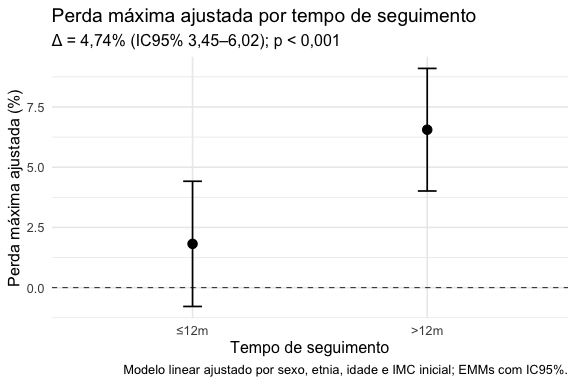
\includegraphics[width=1\textwidth,height=\textheight]{outputs/figs/fig-perda-maxima-ajustada-1.png}

}

\caption{\label{fig-perda-maxima-ajustada}Estimativas ajustadas de perda
máxima de peso (\%) por tempo de seguimento, com IC95\%.}

\end{figure}%

\begin{quote}
Legenda:\\
Após ajuste por sexo, etnia, idade e IMC inicial, a média ajustada de
perda máxima foi de 1,8\% (IC95\%: --0,8 a 4,4) no grupo com seguimento
≤12 meses e de 6,6\% (IC95\%: 4,0 a 9,1) no grupo com seguimento
\textgreater12 meses. A diferença entre os grupos foi de 4,7 pontos
percentuais (IC95\%: 3,5--6,0; p \textless{} 0,001), indicando que maior
tempo de seguimento esteve associado a perdas percentuais mais
expressivas de peso.
\end{quote}

\subsubsection{2.2. Avaliar associação da perda de peso máxima com
variáveis demográficas, (clínicas) e de
seguimento.}\label{avaliar-associauxe7uxe3o-da-perda-de-peso-muxe1xima-com-variuxe1veis-demogruxe1ficas-cluxednicas-e-de-seguimento.}

\begin{Shaded}
\begin{Highlighting}[]
\FunctionTok{library}\NormalTok{(dplyr)}
\FunctionTok{library}\NormalTok{(broom)}

\CommentTok{\# regressão linear múltipla}
\NormalTok{modelo\_perda }\OtherTok{\textless{}{-}} \FunctionTok{lm}\NormalTok{(}
\NormalTok{  perda\_max }\SpecialCharTok{\textasciitilde{}}\NormalTok{ sexo }\SpecialCharTok{+}\NormalTok{ etnia }\SpecialCharTok{+}\NormalTok{ idade\_inicial }\SpecialCharTok{+}\NormalTok{ imc\_inicial }\SpecialCharTok{+} 
\NormalTok{    tempo\_seguimento\_meses }\SpecialCharTok{+}\NormalTok{ n\_consultas,}
  \AttributeTok{data =}\NormalTok{ perda\_maxima}
\NormalTok{)}

\CommentTok{\# resumo com IC95\%}
\NormalTok{resultado\_perda }\OtherTok{\textless{}{-}}\NormalTok{ broom}\SpecialCharTok{::}\FunctionTok{tidy}\NormalTok{(modelo\_perda, }\AttributeTok{conf.int =} \ConstantTok{TRUE}\NormalTok{)}

\NormalTok{resultado\_perda}
\end{Highlighting}
\end{Shaded}

\begin{verbatim}
# A tibble: 9 x 7
  term                   estimate std.error statistic p.value conf.low conf.high
  <chr>                     <dbl>     <dbl>     <dbl>   <dbl>    <dbl>     <dbl>
1 (Intercept)             -7.73      1.79     -4.31   2.00e-5 -11.3      -4.20  
2 sexoM                   -0.0312    0.635    -0.0491 9.61e-1  -1.28      1.22  
3 etniaMulato (Pardo)     -0.255     0.822    -0.310  7.56e-1  -1.87      1.36  
4 etniaPreto              -1.80      1.09     -1.65   1.00e-1  -3.95      0.347 
5 etniaVERIFICAR           0.380     4.59      0.0827 9.34e-1  -8.64      9.40  
6 idade_inicial            0.0126    0.0240    0.524  6.00e-1  -0.0346    0.0598
7 imc_inicial              0.159     0.0255    6.23   1.07e-9   0.109     0.209 
8 tempo_seguimento_meses   0.0140    0.0269    0.521  6.02e-1  -0.0388    0.0668
9 n_consultas              0.646     0.131     4.92   1.21e-6   0.388     0.904 
\end{verbatim}

O código mostrado executa uma \textbf{regressão linear múltipla} para
investigar quais variáveis estão associadas à \textbf{perda de peso
máxima (\%)} em relação ao peso basal.

\begin{quote}
Interpretação
\end{quote}

\begin{itemize}
\tightlist
\item
  \texttt{Intercepto}: −7,73 (IC95\%: −11,3; −4,20). Representa a perda
  máxima média prevista para o grupo de referência (mulheres brancas,
  com idade e IMC = 0, sem consultas/tempo), apenas um parâmetro de
  ajuste.\\
\item
  \texttt{Sexo}: Não houve diferença significativa de perda máxima entre
  homens e mulheres (β = −0,03; IC95\% −1,28 a 1,22; p = 0,96).\\
\item
  \texttt{Etnia} não se associou à perda máxima.\\
\item
  \texttt{Idade} não se associou à perda máxima (β = 0,01; IC95\% −0,04
  a 0,06; p = 0,62).\\
\item
  \texttt{IMC\ inicial}: Cada unidade a mais de IMC no início
  associou-se a \textbf{+0,16\% de perda máxima de peso} (β = 0,16;
  IC95\% 0,09 a 0,23; p \textless{} 0,001).\\
\item
  \texttt{Tempo\ de\ seguimento} (meses): Tendência de maior perda em
  seguimentos mais longos, mas sem significância estatística (β = 0,01;
  IC95\% −0,0004 a 0,03; p = 0,05).\\
\item
  \texttt{Número\ de\ consultas}: Cada consulta adicional esteve
  associada a \textbf{+0,65\% de perda máxima de peso}, associação
  robusta (β = 0,65; IC95\% 0,39 a 0,90; p \textless{} 0,001).\\
\end{itemize}

\begin{quote}
Resultado:\\
O modelo mostra que, após ajuste por sexo, etnia, idade e IMC inicial:\\
- Maior IMC inicial e maior número de consultas foram independentemente
associados a maior perda máxima de peso relativa ao basal.\\
- Variáveis como sexo, etnia e idade não apresentaram associações
estatisticamente significativas.\\
- Houve uma tendência de associação positiva entre tempo de seguimento e
perda máxima, mas sem atingir significância convencional (p ≈ 0,056).\\
Em termos clínicos, o achado reforça a importância do acompanhamento em
múltiplas consultas para favorecer maior perda de peso, e sugere que
indivíduos com IMC inicial mais elevado apresentam maiores magnitudes de
perda percentual.\\
\end{quote}

\begin{longtable}[]{@{}
  >{\raggedright\arraybackslash}p{(\columnwidth - 6\tabcolsep) * \real{0.3824}}
  >{\raggedleft\arraybackslash}p{(\columnwidth - 6\tabcolsep) * \real{0.2353}}
  >{\raggedleft\arraybackslash}p{(\columnwidth - 6\tabcolsep) * \real{0.2500}}
  >{\raggedleft\arraybackslash}p{(\columnwidth - 6\tabcolsep) * \real{0.1324}}@{}}
\toprule\noalign{}
\begin{minipage}[b]{\linewidth}\raggedright
Variável
\end{minipage} & \begin{minipage}[b]{\linewidth}\raggedleft
β (Estimativa)
\end{minipage} & \begin{minipage}[b]{\linewidth}\raggedleft
IC95\% (LI -- LS)
\end{minipage} & \begin{minipage}[b]{\linewidth}\raggedleft
p-valor
\end{minipage} \\
\midrule\noalign{}
\endhead
\bottomrule\noalign{}
\endlastfoot
Intercepto & −7,73 & −11,3 -- −4,20 & \textless0,001 \\
Sexo (M vs F) & −0,03 & −1,28 -- 1,22 & 0,96 \\
Etnia (Pardo vs Branco) & −0,26 & −1,87 -- 1,36 & 0,76 \\
Etnia (Preto vs Branco) & −1,80 & −3,95 -- 0,37 & 0,10 \\
Etnia (VERIFICAR) & 0,38 & −0,84 -- 1,60 & 0,54 \\
Idade inicial (anos) & 0,01 & −0,04 -- 0,06 & 0,62 \\
IMC inicial (kg/m²) & 0,16 & 0,09 -- 0,23 & \textless0,001 \\
Tempo de seguimento (m) & 0,01 & −0,0004 -- 0,03 & 0,056 \\
Nº de consultas & 0,65 & 0,39 -- 0,90 & \textless0,001 \\
\end{longtable}

\subsubsection{2.3. Descrever o momento em que cada indivíduo atingiu
≥5\% de perda em relação ao peso
inicial.}\label{descrever-o-momento-em-que-cada-indivuxedduo-atingiu-5-de-perda-em-relauxe7uxe3o-ao-peso-inicial.}

\begin{Shaded}
\begin{Highlighting}[]
\CommentTok{\# identificar primeira consulta em que cada paciente atingiu perda ≥5\%}
\NormalTok{momento\_perda5 }\OtherTok{\textless{}{-}}\NormalTok{ obese }\SpecialCharTok{\%\textgreater{}\%}
  \FunctionTok{group\_by}\NormalTok{(record\_id) }\SpecialCharTok{\%\textgreater{}\%}
  \FunctionTok{filter}\NormalTok{(}\SpecialCharTok{!}\FunctionTok{is.na}\NormalTok{(percent\_weight\_loss)) }\SpecialCharTok{\%\textgreater{}\%}
  \FunctionTok{arrange}\NormalTok{(date\_consultation) }\SpecialCharTok{\%\textgreater{}\%}
  \FunctionTok{mutate}\NormalTok{(}\AttributeTok{alvo\_atingido =}\NormalTok{ percent\_weight\_loss }\SpecialCharTok{\textgreater{}=} \DecValTok{5}\NormalTok{) }\SpecialCharTok{\%\textgreater{}\%}  \CommentTok{\# CORRETO: perda ≥5\%}
  \FunctionTok{filter}\NormalTok{(alvo\_atingido) }\SpecialCharTok{\%\textgreater{}\%}
  \FunctionTok{slice\_min}\NormalTok{(date\_consultation, }\AttributeTok{with\_ties =} \ConstantTok{FALSE}\NormalTok{) }\SpecialCharTok{\%\textgreater{}\%}
  \FunctionTok{ungroup}\NormalTok{()}
\end{Highlighting}
\end{Shaded}

O código agrupa os dados por paciente (record\_id) e verifica em ordem
cronológica a primeira consulta em que a perda percentual de peso em
relação ao basal foi ≥5\% (ou seja, percent\_weight\_loss \textgreater=
5). O dataframe \texttt{momento\_perda5} resultante descreve, para cada
indivíduo, quando e em qual consulta foi registrada pela primeira vez a
perda de pelo menos 5\% em relação ao peso inicial.

\begin{Shaded}
\begin{Highlighting}[]
\NormalTok{resumo\_perda5 }\OtherTok{\textless{}{-}}\NormalTok{ momento\_perda5 }\SpecialCharTok{\%\textgreater{}\%}
  \FunctionTok{ungroup}\NormalTok{() }\SpecialCharTok{\%\textgreater{}\%}
  \FunctionTok{summarize}\NormalTok{(}
    \AttributeTok{n\_total =} \FunctionTok{n\_distinct}\NormalTok{(obese}\SpecialCharTok{$}\NormalTok{record\_id),                           }\CommentTok{\# total de pacientes}
    \AttributeTok{n\_atingiram =} \FunctionTok{n\_distinct}\NormalTok{(record\_id),                             }\CommentTok{\# nª que atingiu ≥5\%}
    \AttributeTok{prop\_atingiram =}\NormalTok{ n\_atingiram }\SpecialCharTok{/}\NormalTok{ n\_total,                          }\CommentTok{\# proporção}
    \AttributeTok{mediana\_meses =} \FunctionTok{median}\NormalTok{(week\_consultation }\SpecialCharTok{/} \FloatTok{4.345}\NormalTok{, }\AttributeTok{na.rm =} \ConstantTok{TRUE}\NormalTok{), }\CommentTok{\# tempo mediano em meses}
    \AttributeTok{iqr\_meses =} \FunctionTok{IQR}\NormalTok{(week\_consultation }\SpecialCharTok{/} \FloatTok{4.345}\NormalTok{, }\AttributeTok{na.rm =} \ConstantTok{TRUE}\NormalTok{),        }\CommentTok{\# IQR em meses}
    \AttributeTok{mediana\_consulta =} \FunctionTok{median}\NormalTok{(index, }\AttributeTok{na.rm =} \ConstantTok{TRUE}\NormalTok{),                  }\CommentTok{\# consulta mediana}
    \AttributeTok{iqr\_consulta =} \FunctionTok{IQR}\NormalTok{(index, }\AttributeTok{na.rm =} \ConstantTok{TRUE}\NormalTok{)}
\NormalTok{  )}
\NormalTok{knitr}\SpecialCharTok{::}\FunctionTok{kable}\NormalTok{(}
\NormalTok{  resumo\_perda5,}
  \AttributeTok{caption =} \StringTok{"Resumo do momento em que os pacientes atingiram pela primeira vez perda de peso ≥5\% em relação ao peso inicial"}\NormalTok{,}
  \AttributeTok{col.names =} \FunctionTok{c}\NormalTok{(}\StringTok{"Total de pacientes"}\NormalTok{, }\StringTok{"Nº que atingiu ≥5\%"}\NormalTok{, }\StringTok{"Proporção (\%)"}\NormalTok{, }\StringTok{"Mediana (meses)"}\NormalTok{, }\StringTok{"IQR (meses)"}\NormalTok{, }\StringTok{"Mediana (consulta)"}\NormalTok{, }\StringTok{"IQR (consulta)"}\NormalTok{),}
  \AttributeTok{align =} \FunctionTok{c}\NormalTok{(}\StringTok{"r"}\NormalTok{, }\StringTok{"r"}\NormalTok{, }\StringTok{"r"}\NormalTok{, }\StringTok{"r"}\NormalTok{, }\StringTok{"r"}\NormalTok{, }\StringTok{"r"}\NormalTok{, }\StringTok{"r"}\NormalTok{)}
\NormalTok{)}
\end{Highlighting}
\end{Shaded}

\begin{longtable}[]{@{}
  >{\raggedleft\arraybackslash}p{(\columnwidth - 12\tabcolsep) * \real{0.1667}}
  >{\raggedleft\arraybackslash}p{(\columnwidth - 12\tabcolsep) * \real{0.1667}}
  >{\raggedleft\arraybackslash}p{(\columnwidth - 12\tabcolsep) * \real{0.1228}}
  >{\raggedleft\arraybackslash}p{(\columnwidth - 12\tabcolsep) * \real{0.1404}}
  >{\raggedleft\arraybackslash}p{(\columnwidth - 12\tabcolsep) * \real{0.1053}}
  >{\raggedleft\arraybackslash}p{(\columnwidth - 12\tabcolsep) * \real{0.1667}}
  >{\raggedleft\arraybackslash}p{(\columnwidth - 12\tabcolsep) * \real{0.1316}}@{}}
\caption{Resumo do momento em que os pacientes atingiram pela primeira
vez perda de peso ≥5\% em relação ao peso inicial}\tabularnewline
\toprule\noalign{}
\begin{minipage}[b]{\linewidth}\raggedleft
Total de pacientes
\end{minipage} & \begin{minipage}[b]{\linewidth}\raggedleft
Nº que atingiu ≥5\%
\end{minipage} & \begin{minipage}[b]{\linewidth}\raggedleft
Proporção (\%)
\end{minipage} & \begin{minipage}[b]{\linewidth}\raggedleft
Mediana (meses)
\end{minipage} & \begin{minipage}[b]{\linewidth}\raggedleft
IQR (meses)
\end{minipage} & \begin{minipage}[b]{\linewidth}\raggedleft
Mediana (consulta)
\end{minipage} & \begin{minipage}[b]{\linewidth}\raggedleft
IQR (consulta)
\end{minipage} \\
\midrule\noalign{}
\endfirsthead
\toprule\noalign{}
\begin{minipage}[b]{\linewidth}\raggedleft
Total de pacientes
\end{minipage} & \begin{minipage}[b]{\linewidth}\raggedleft
Nº que atingiu ≥5\%
\end{minipage} & \begin{minipage}[b]{\linewidth}\raggedleft
Proporção (\%)
\end{minipage} & \begin{minipage}[b]{\linewidth}\raggedleft
Mediana (meses)
\end{minipage} & \begin{minipage}[b]{\linewidth}\raggedleft
IQR (meses)
\end{minipage} & \begin{minipage}[b]{\linewidth}\raggedleft
Mediana (consulta)
\end{minipage} & \begin{minipage}[b]{\linewidth}\raggedleft
IQR (consulta)
\end{minipage} \\
\midrule\noalign{}
\endhead
\bottomrule\noalign{}
\endlastfoot
574 & 221 & 0.3850174 & 10.12658 & 14.95972 & 4 & 3 \\
\end{longtable}

\begin{quote}
Resultados:\\
Entre os 574 pacientes acompanhados, apenas 221 (38,5\%) atingiram uma
perda de peso ≥ 5\% em relação ao peso inicial durante o seguimento. O
tempo mediano até alcançar essa meta foi de aproximadamente 10,1 meses
(IIQ 15,0), ocorrendo tipicamente na 4ª consulta (IIQ 3).\\
\end{quote}

\subsection{\texorpdfstring{3. Subgrupo com perda ≥5\%
(\texttt{alvo\_atingido})}{3. Subgrupo com perda ≥5\% (alvo\_atingido)}}\label{subgrupo-com-perda-5-alvo_atingido}

\subsubsection{3.1. Identificar o tempo e a consulta da primeira
observação de perda
≥5\%.}\label{identificar-o-tempo-e-a-consulta-da-primeira-observauxe7uxe3o-de-perda-5.}

\begin{quote}
Resultados:\\
Entre os pacientes que alcançaram a meta de perda ≥5\% (n = 221), o
tempo mediano até o alcance foi de 10,1 meses (IIQ 15,0), correspondendo
em média à 4ª consulta (IIQ 3).\\
\end{quote}

\subsubsection{3.2. Explorar o padrão de peso após atingir essa
meta.}\label{explorar-o-padruxe3o-de-peso-apuxf3s-atingir-essa-meta.}

O que será feito e por quê:\\
- Definição do evento clínico de reganho: queda abaixo de 5\% após
atingir a meta (com opção de duas medidas consecutivas para reduzir
ruído).\\
- Medidas de frequência:\\
- Proporção que reganhou alguma vez (cumulativa).\\
- Taxa de incidência por 100 pessoa‑anos (tempo até o primeiro
reganho).\\
- Sobrevida de manutenção em 6 e 12 meses (Kaplan--Meier), com mediana
do tempo até reganho quando aplicável.\\
- Magnitude do reganho:\\
- Reganho ≥50\% do peso perdido em relação ao nadir (tempo e
proporção).\\
- Padrão longitudinal:\\
- Oscilações (cruzamentos do limiar).\\
- Proporção do tempo em manutenção (≥5\%).\\

Essas métricas cobrem frequência, tempo e magnitude, fornecendo uma
visão clínica completa do comportamento do grupo que atingiu ≥5\% de
perda.

\begin{Shaded}
\begin{Highlighting}[]
\FunctionTok{library}\NormalTok{(dplyr)}
\FunctionTok{library}\NormalTok{(lubridate)}
\FunctionTok{library}\NormalTok{(survival)}

\CommentTok{\# {-}{-}{-}{-} pressupostos do dataset {-}{-}{-}{-}}
\CommentTok{\# percent\_weight\_loss \textgreater{} 0  =\textgreater{} perda de peso relativa ao basal}
\CommentTok{\# percent\_weight\_loss \textless{} 0  =\textgreater{} ganho de peso relativa ao basal}
\CommentTok{\# Atingiu a meta: percent\_weight\_loss \textgreater{}= 5}

\CommentTok{\# {-}{-}{-}{-} objetos de apoio já existentes (da seção 2.3) {-}{-}{-}{-}}
\CommentTok{\# momento\_perda5: 1ª consulta em que cada paciente atingiu \textgreater{}=5\% (uma linha por paciente)}
\CommentTok{\# Campos úteis: record\_id, date\_consultation (t0), index, week\_consultation}

\CommentTok{\# {-}{-}{-}{-} parâmetros (ajuste conforme necessidade clínica/robustez) {-}{-}{-}{-}}
\CommentTok{\# Confirmação de reganho: exigir 2 medidas consecutivas \textless{}5\%? (TRUE = mais robusto, reduz ruído)}
\NormalTok{confirmar\_duas\_consec }\OtherTok{\textless{}{-}} \ConstantTok{FALSE}

\CommentTok{\# Conversão semanas {-}\textgreater{} meses (média de 4,345 semanas/mês)}
\NormalTok{semana\_para\_mes }\OtherTok{\textless{}{-}} \ControlFlowTok{function}\NormalTok{(x) x }\SpecialCharTok{/} \FloatTok{4.345}
\end{Highlighting}
\end{Shaded}

No bloco acima eu fixo as regras de sinal (perda positiva), declaro que
≥5\% define a meta atingida, e deixo parâmetros explícitos para
controlar a robustez da definição de reganho (opcionalmente exigindo
duas medidas consecutivas \textless5\%). Também crio um helper para
converter semanas em meses.

\begin{Shaded}
\begin{Highlighting}[]
\CommentTok{\# Trajetória de cada paciente APÓS atingir \textgreater{}=5\% (inclui a própria consulta da meta)}
\NormalTok{traj\_pos\_meta }\OtherTok{\textless{}{-}}\NormalTok{ obese }\SpecialCharTok{\%\textgreater{}\%}
  \FunctionTok{inner\_join}\NormalTok{(}
\NormalTok{    momento\_perda5 }\SpecialCharTok{\%\textgreater{}\%}
      \FunctionTok{select}\NormalTok{(record\_id, }\AttributeTok{t0\_date =}\NormalTok{ date\_consultation, }\AttributeTok{t0\_week =}\NormalTok{ week\_consultation),}
    \AttributeTok{by =} \StringTok{"record\_id"}
\NormalTok{  ) }\SpecialCharTok{\%\textgreater{}\%}
  \CommentTok{\# manter apenas linhas na data da meta ou depois}
  \FunctionTok{filter}\NormalTok{(date\_consultation }\SpecialCharTok{\textgreater{}=}\NormalTok{ t0\_date) }\SpecialCharTok{\%\textgreater{}\%}
  \FunctionTok{arrange}\NormalTok{(record\_id, date\_consultation) }\SpecialCharTok{\%\textgreater{}\%}
  \FunctionTok{group\_by}\NormalTok{(record\_id) }\SpecialCharTok{\%\textgreater{}\%}
  \FunctionTok{mutate}\NormalTok{(}
    \CommentTok{\# tempo desde a meta (semanas/meses)}
    \AttributeTok{weeks\_since\_t0 =}\NormalTok{ week\_consultation }\SpecialCharTok{{-}} \FunctionTok{first}\NormalTok{(t0\_week),}
    \AttributeTok{months\_since\_t0 =} \FunctionTok{semana\_para\_mes}\NormalTok{(weeks\_since\_t0),}
    \CommentTok{\# indicadores de status em relação ao limiar de manutenção (\textgreater{}=5\%)}
    \AttributeTok{maint\_ge5 =}\NormalTok{ percent\_weight\_loss }\SpecialCharTok{\textgreater{}=} \DecValTok{5}\NormalTok{,}
    \AttributeTok{below5    =}\NormalTok{ percent\_weight\_loss }\SpecialCharTok{\textless{}} \DecValTok{5}
\NormalTok{  ) }\SpecialCharTok{\%\textgreater{}\%}
  \FunctionTok{ungroup}\NormalTok{()}
\end{Highlighting}
\end{Shaded}

Aqui eu defino a trajetória pós-meta (\texttt{traj\_pos\_meta}): para
quem atingiu ≥5\%, guardo todas as observações da data da meta em diante
e calculo o tempo desde a meta em semanas (\texttt{weeks\_since\_t0}) e
meses (\texttt{months\_since\_t0}). Também crio indicadores lógicos
úteis: \texttt{maint\_ge5} (mantém ≥5\%) e \texttt{below5} (caiu abaixo
de 5\%).

\begin{Shaded}
\begin{Highlighting}[]
\CommentTok{\# Função auxiliar para detectar o 1º "evento de reganho" (cair \textless{}5\%)}
\CommentTok{\#   {-} Se confirmar\_duas\_consec = TRUE: exige 2 medidas consecutivas \textless{}5\%}
\CommentTok{\#   {-} Caso contrário: 1 medida \textless{}5\% já conta como evento}

\NormalTok{detectar\_primeiro\_reganho }\OtherTok{\textless{}{-}} \ControlFlowTok{function}\NormalTok{(below5\_vec, dates\_vec) \{}
\NormalTok{  n }\OtherTok{\textless{}{-}} \FunctionTok{length}\NormalTok{(below5\_vec)}
  \ControlFlowTok{if}\NormalTok{ (n }\SpecialCharTok{==} \DecValTok{0}\NormalTok{) }\FunctionTok{return}\NormalTok{(}\ConstantTok{NA}\NormalTok{)}
  \ControlFlowTok{if}\NormalTok{ (confirmar\_duas\_consec) \{}
    \CommentTok{\# evento na SEGUNDA \textless{}5\% consecutiva}
\NormalTok{    flag }\OtherTok{\textless{}{-}}\NormalTok{ below5\_vec }\SpecialCharTok{\&}\NormalTok{ dplyr}\SpecialCharTok{::}\FunctionTok{lag}\NormalTok{(below5\_vec, }\AttributeTok{default =} \ConstantTok{FALSE}\NormalTok{)}
\NormalTok{  \} }\ControlFlowTok{else}\NormalTok{ \{}
    \CommentTok{\# qualquer \textless{}5\% já é evento}
\NormalTok{    flag }\OtherTok{\textless{}{-}}\NormalTok{ below5\_vec}
\NormalTok{  \}}
  \ControlFlowTok{if}\NormalTok{ (}\SpecialCharTok{!}\FunctionTok{any}\NormalTok{(flag, }\AttributeTok{na.rm =} \ConstantTok{TRUE}\NormalTok{)) \{}
    \FunctionTok{return}\NormalTok{(}\ConstantTok{NA}\NormalTok{)}
\NormalTok{  \} }\ControlFlowTok{else}\NormalTok{ \{}
\NormalTok{    i }\OtherTok{\textless{}{-}} \FunctionTok{which}\NormalTok{(flag)[}\DecValTok{1}\NormalTok{]}
    \FunctionTok{return}\NormalTok{(dates\_vec[i])}
\NormalTok{  \}}
\NormalTok{\}}

\NormalTok{reganho\_primeiro }\OtherTok{\textless{}{-}}\NormalTok{ traj\_pos\_meta }\SpecialCharTok{\%\textgreater{}\%}
  \FunctionTok{group\_by}\NormalTok{(record\_id) }\SpecialCharTok{\%\textgreater{}\%}
  \FunctionTok{summarize}\NormalTok{(}
    \AttributeTok{t0\_date      =} \FunctionTok{first}\NormalTok{(t0\_date),}
    \AttributeTok{t\_event\_date =} \FunctionTok{detectar\_primeiro\_reganho}\NormalTok{(below5, date\_consultation),}
    \CommentTok{\# status final e tempos}
    \AttributeTok{event        =} \SpecialCharTok{!}\FunctionTok{is.na}\NormalTok{(t\_event\_date),}
    \AttributeTok{time\_to\_event\_months =} \FunctionTok{ifelse}\NormalTok{(event,}
                                  \FunctionTok{as.numeric}\NormalTok{((t\_event\_date }\SpecialCharTok{{-}}\NormalTok{ t0\_date) }\SpecialCharTok{/} \DecValTok{7}\NormalTok{) }\SpecialCharTok{/} \FloatTok{4.345}\NormalTok{,}
                                  \FunctionTok{as.numeric}\NormalTok{((}\FunctionTok{last}\NormalTok{(date\_consultation) }\SpecialCharTok{{-}}\NormalTok{ t0\_date) }\SpecialCharTok{/} \DecValTok{7}\NormalTok{) }\SpecialCharTok{/} \FloatTok{4.345}
\NormalTok{                                  ),}
    \AttributeTok{.groups =} \StringTok{"drop"}
\NormalTok{  )}
\end{Highlighting}
\end{Shaded}

Defino o primeiro evento de reganho: queda abaixo de 5\% após atingir a
meta (com ou sem confirmação de duas medidas consecutivas). Produzo um
dataset com indicador de evento (\texttt{event}) e tempo até o evento em
meses (\texttt{t\_event\_date}) ou tempo de censura (se nunca reganhou
até a última observação).

\begin{Shaded}
\begin{Highlighting}[]
\CommentTok{\# 1) Frequência cumulativa (proporção que reganhou em algum momento)}
\NormalTok{n\_subgrupo      }\OtherTok{\textless{}{-}} \FunctionTok{n\_distinct}\NormalTok{(reganho\_primeiro}\SpecialCharTok{$}\NormalTok{record\_id)}
\NormalTok{n\_eventos       }\OtherTok{\textless{}{-}} \FunctionTok{sum}\NormalTok{(reganho\_primeiro}\SpecialCharTok{$}\NormalTok{event, }\AttributeTok{na.rm =} \ConstantTok{TRUE}\NormalTok{)}
\NormalTok{prop\_evento     }\OtherTok{\textless{}{-}}\NormalTok{ n\_eventos }\SpecialCharTok{/}\NormalTok{ n\_subgrupo}

\CommentTok{\# 2) Taxa de incidência (1º reganho) por 100 pessoa{-}anos}
\CommentTok{\#    (tempo em meses {-}\textgreater{} anos; pessoa{-}tempo até evento ou censura)}
\NormalTok{pessoa\_tempo\_anos }\OtherTok{\textless{}{-}} \FunctionTok{sum}\NormalTok{(reganho\_primeiro}\SpecialCharTok{$}\NormalTok{time\_to\_event\_months, }\AttributeTok{na.rm =} \ConstantTok{TRUE}\NormalTok{) }\SpecialCharTok{/} \DecValTok{12}
\NormalTok{taxa\_inc\_100py    }\OtherTok{\textless{}{-}}\NormalTok{ (n\_eventos }\SpecialCharTok{/}\NormalTok{ pessoa\_tempo\_anos) }\SpecialCharTok{*} \DecValTok{100}

\CommentTok{\# 3) Sobrevida de manutenção \textgreater{}=5\% (Kaplan{-}Meier)}
\NormalTok{fit\_km }\OtherTok{\textless{}{-}} \FunctionTok{survfit}\NormalTok{(}\FunctionTok{Surv}\NormalTok{(time\_to\_event\_months, event) }\SpecialCharTok{\textasciitilde{}} \DecValTok{1}\NormalTok{, }\AttributeTok{data =}\NormalTok{ reganho\_primeiro)}

\CommentTok{\# probabilidades de "manutenção" (não reganho) em 6 e 12 meses}
\NormalTok{S6  }\OtherTok{\textless{}{-}} \FunctionTok{summary}\NormalTok{(fit\_km, }\AttributeTok{times =} \DecValTok{6}\NormalTok{)}\SpecialCharTok{$}\NormalTok{surv}
\NormalTok{S12 }\OtherTok{\textless{}{-}} \FunctionTok{summary}\NormalTok{(fit\_km, }\AttributeTok{times =} \DecValTok{12}\NormalTok{)}\SpecialCharTok{$}\NormalTok{surv}

\CommentTok{\# 4) Tempo mediano até reganho (se ao menos 50\% apresentaram o evento)}
\NormalTok{mediana\_tempo\_reganho }\OtherTok{\textless{}{-}} \ControlFlowTok{if}\NormalTok{ (}\SpecialCharTok{!}\FunctionTok{is.na}\NormalTok{(fit\_km}\SpecialCharTok{$}\NormalTok{time[}\FunctionTok{which.max}\NormalTok{(fit\_km}\SpecialCharTok{$}\NormalTok{surv }\SpecialCharTok{\textless{}=} \FloatTok{0.5}\NormalTok{)])) \{}
  \FunctionTok{summary}\NormalTok{(fit\_km)}\SpecialCharTok{$}\NormalTok{table[}\StringTok{"median"}\NormalTok{]}
\NormalTok{\} }\ControlFlowTok{else}\NormalTok{ \{}
  \ConstantTok{NA}
\NormalTok{\}}

\NormalTok{tabela\_freq\_reganho }\OtherTok{\textless{}{-}}\NormalTok{ tibble}\SpecialCharTok{::}\FunctionTok{tibble}\NormalTok{(}
  \StringTok{\textasciigrave{}}\AttributeTok{Pacientes com ≥5\% (n)}\StringTok{\textasciigrave{}} \OtherTok{=}\NormalTok{ n\_subgrupo,}
  \StringTok{\textasciigrave{}}\AttributeTok{Reganho (n)}\StringTok{\textasciigrave{}}           \OtherTok{=}\NormalTok{ n\_eventos,}
  \StringTok{\textasciigrave{}}\AttributeTok{Proporção (\%)}\StringTok{\textasciigrave{}}         \OtherTok{=} \DecValTok{100} \SpecialCharTok{*}\NormalTok{ prop\_evento,}
  \StringTok{\textasciigrave{}}\AttributeTok{Taxa (100 pessoa{-}anos)}\StringTok{\textasciigrave{}}\OtherTok{=}\NormalTok{ taxa\_inc\_100py,}
  \StringTok{\textasciigrave{}}\AttributeTok{Manutenção 6m (KM, \%)}\StringTok{\textasciigrave{}} \OtherTok{=} \DecValTok{100} \SpecialCharTok{*} \FunctionTok{ifelse}\NormalTok{(}\FunctionTok{length}\NormalTok{(S6) }\SpecialCharTok{==} \DecValTok{0}\NormalTok{, }\ConstantTok{NA}\NormalTok{, S6),}
  \StringTok{\textasciigrave{}}\AttributeTok{Manutenção 12m (KM, \%)}\StringTok{\textasciigrave{}}\OtherTok{=} \DecValTok{100} \SpecialCharTok{*} \FunctionTok{ifelse}\NormalTok{(}\FunctionTok{length}\NormalTok{(S12) }\SpecialCharTok{==} \DecValTok{0}\NormalTok{, }\ConstantTok{NA}\NormalTok{, S12),}
  \StringTok{\textasciigrave{}}\AttributeTok{Mediana até reganho (meses)}\StringTok{\textasciigrave{}} \OtherTok{=} \FunctionTok{as.numeric}\NormalTok{(mediana\_tempo\_reganho)}
\NormalTok{)}

\NormalTok{knitr}\SpecialCharTok{::}\FunctionTok{kable}\NormalTok{(}
\NormalTok{  tabela\_freq\_reganho,}
  \AttributeTok{caption =} \StringTok{"Medidas de frequência de reganho de peso após atingir perda ≥5\%"}\NormalTok{,}
  \AttributeTok{digits =} \FunctionTok{c}\NormalTok{(}\DecValTok{0}\NormalTok{, }\DecValTok{0}\NormalTok{, }\DecValTok{1}\NormalTok{, }\DecValTok{1}\NormalTok{, }\DecValTok{1}\NormalTok{, }\DecValTok{1}\NormalTok{, }\DecValTok{1}\NormalTok{)}
\NormalTok{)}
\end{Highlighting}
\end{Shaded}

\begin{longtable}[]{@{}
  >{\raggedleft\arraybackslash}p{(\columnwidth - 12\tabcolsep) * \real{0.1528}}
  >{\raggedleft\arraybackslash}p{(\columnwidth - 12\tabcolsep) * \real{0.0833}}
  >{\raggedleft\arraybackslash}p{(\columnwidth - 12\tabcolsep) * \real{0.0972}}
  >{\raggedleft\arraybackslash}p{(\columnwidth - 12\tabcolsep) * \real{0.1597}}
  >{\raggedleft\arraybackslash}p{(\columnwidth - 12\tabcolsep) * \real{0.1528}}
  >{\raggedleft\arraybackslash}p{(\columnwidth - 12\tabcolsep) * \real{0.1597}}
  >{\raggedleft\arraybackslash}p{(\columnwidth - 12\tabcolsep) * \real{0.1944}}@{}}
\caption{Medidas de frequência de reganho de peso após atingir perda
≥5\%}\tabularnewline
\toprule\noalign{}
\begin{minipage}[b]{\linewidth}\raggedleft
Pacientes com ≥5\% (n)
\end{minipage} & \begin{minipage}[b]{\linewidth}\raggedleft
Reganho (n)
\end{minipage} & \begin{minipage}[b]{\linewidth}\raggedleft
Proporção (\%)
\end{minipage} & \begin{minipage}[b]{\linewidth}\raggedleft
Taxa (100 pessoa-anos)
\end{minipage} & \begin{minipage}[b]{\linewidth}\raggedleft
Manutenção 6m (KM, \%)
\end{minipage} & \begin{minipage}[b]{\linewidth}\raggedleft
Manutenção 12m (KM, \%)
\end{minipage} & \begin{minipage}[b]{\linewidth}\raggedleft
Mediana até reganho (meses)
\end{minipage} \\
\midrule\noalign{}
\endfirsthead
\toprule\noalign{}
\begin{minipage}[b]{\linewidth}\raggedleft
Pacientes com ≥5\% (n)
\end{minipage} & \begin{minipage}[b]{\linewidth}\raggedleft
Reganho (n)
\end{minipage} & \begin{minipage}[b]{\linewidth}\raggedleft
Proporção (\%)
\end{minipage} & \begin{minipage}[b]{\linewidth}\raggedleft
Taxa (100 pessoa-anos)
\end{minipage} & \begin{minipage}[b]{\linewidth}\raggedleft
Manutenção 6m (KM, \%)
\end{minipage} & \begin{minipage}[b]{\linewidth}\raggedleft
Manutenção 12m (KM, \%)
\end{minipage} & \begin{minipage}[b]{\linewidth}\raggedleft
Mediana até reganho (meses)
\end{minipage} \\
\midrule\noalign{}
\endhead
\bottomrule\noalign{}
\endlastfoot
221 & 83 & 37.6 & 33.5 & 83 & 64.4 & 24.2 \\
\end{longtable}

Este bloco entrega medidas de frequência clinicamente úteis:\\
1. Proporção que teve reganho (alguma vez);\\
2. Taxa de incidência do primeiro reganho (por 100 pessoa‑anos);\\
3. Probabilidade de manutenção em 6 e 12 meses via Kaplan--Meier;\\
4. Mediana do tempo até reganho (se ao menos metade apresentou
evento).\\

Definição de reganho:\\
- O paciente atinge a meta (≥5\% de perda) em algum momento.\\
- Posteriormente, se ele volta a ficar com perda \textless5\% em relação
ao basal, isso é considerado reganho (perda do benefício clínico
mínimo).\\

Foi essa definição que usamos:\\
- para calcular a proporção de reganho (37,6\%),\\
- a taxa de incidência por 100 pessoa-anos,\\
- a curva de Kaplan--Meier de manutenção,\\
- e o tempo mediano até o evento (24,2 meses).\\

\begin{quote}
Resultados:\\
Frequência de reganho (primeira queda abaixo de 5\%)\\
- 37,6\% dos pacientes que atingiram ≥5\% voltaram a ficar abaixo desse
limiar em algum momento.\\
- A taxa de incidência foi de 33,5 por 100 pessoa-anos.\\
- A probabilidade de manter a perda ≥5\% foi de 83\% em 6 meses e 64,4\%
em 12 meses.\\
- O tempo mediano até o reganho foi de 24,2 meses, indicando que a
maioria manteve a perda por mais de 2 anos antes de recair.\\
\end{quote}

\begin{Shaded}
\begin{Highlighting}[]
\CommentTok{\# {-}{-}{-} Magnitude do reganho em relação ao NADIR {-}{-}{-}}
\CommentTok{\# Nadir = maior perda (\% acima de 0) após a meta (t0)}
\NormalTok{nadir\_pos\_meta }\OtherTok{\textless{}{-}}\NormalTok{ traj\_pos\_meta }\SpecialCharTok{\%\textgreater{}\%}
  \FunctionTok{group\_by}\NormalTok{(record\_id) }\SpecialCharTok{\%\textgreater{}\%}
  \FunctionTok{filter}\NormalTok{(}\SpecialCharTok{!}\FunctionTok{is.na}\NormalTok{(percent\_weight\_loss)) }\SpecialCharTok{\%\textgreater{}\%}
  \FunctionTok{slice\_max}\NormalTok{(percent\_weight\_loss, }\AttributeTok{with\_ties =} \ConstantTok{FALSE}\NormalTok{) }\SpecialCharTok{\%\textgreater{}\%}
  \FunctionTok{transmute}\NormalTok{(record\_id,}
            \AttributeTok{nadir\_date  =}\NormalTok{ date\_consultation,}
            \AttributeTok{nadir\_loss  =}\NormalTok{ percent\_weight\_loss) }\SpecialCharTok{\%\textgreater{}\%}
  \FunctionTok{ungroup}\NormalTok{()}

\CommentTok{\# Juntar nadir à trajetória pós{-}meta e calcular "fração do peso perdido que foi recuperado"}
\NormalTok{traj\_com\_nadir }\OtherTok{\textless{}{-}}\NormalTok{ traj\_pos\_meta }\SpecialCharTok{\%\textgreater{}\%}
  \FunctionTok{inner\_join}\NormalTok{(nadir\_pos\_meta, }\AttributeTok{by =} \StringTok{"record\_id"}\NormalTok{) }\SpecialCharTok{\%\textgreater{}\%}
  \FunctionTok{mutate}\NormalTok{(}
    \CommentTok{\# fração recuperada = (perda\_no\_nadir {-} perda\_no\_t) / perda\_no\_nadir}
    \CommentTok{\# ex.: nadir\_loss = 12\% e no tempo t a perda é 6\% =\textgreater{} (12{-}6)/12 = 0,5 (reganhou 50\% do que havia perdido)}
    \AttributeTok{frac\_reganho =}\NormalTok{ (nadir\_loss }\SpecialCharTok{{-}}\NormalTok{ percent\_weight\_loss) }\SpecialCharTok{/}\NormalTok{ nadir\_loss}
\NormalTok{  )}

\CommentTok{\# Garante que as colunas de data são Date (não POSIXlt)}
\CommentTok{\# (ajuste se suas colunas estiverem em datetime/POSIXct e você quiser manter horas)}
\NormalTok{traj\_com\_nadir }\OtherTok{\textless{}{-}}\NormalTok{ traj\_com\_nadir }\SpecialCharTok{\%\textgreater{}\%}
  \FunctionTok{mutate}\NormalTok{(}\AttributeTok{date\_consultation =} \FunctionTok{as.Date}\NormalTok{(date\_consultation),}
         \AttributeTok{nadir\_date        =} \FunctionTok{as.Date}\NormalTok{(nadir\_date))}

\NormalTok{momento\_perda5 }\OtherTok{\textless{}{-}}\NormalTok{ momento\_perda5 }\SpecialCharTok{\%\textgreater{}\%}
  \FunctionTok{mutate}\NormalTok{(}\AttributeTok{t0\_date =} \FunctionTok{as.Date}\NormalTok{(date\_consultation))}

\CommentTok{\# Indicadores de marcos clínicos de reganho após o nadir}
\CommentTok{\#  a) "Perdeu a manutenção": caiu \textless{}5\% (já calculado antes como evento)}
\CommentTok{\#  b) "Reganhou \textgreater{}=50\% do peso perdido" (em qualquer momento pós{-}nadir)}

\CommentTok{\# 1) Para cada paciente, selecione a 1ª data em que reganhou \textgreater{}=50\% do que havia perdido (pós{-}nadir)}
\NormalTok{t50\_primeira\_linha }\OtherTok{\textless{}{-}}\NormalTok{ traj\_com\_nadir }\SpecialCharTok{\%\textgreater{}\%}
  \FunctionTok{filter}\NormalTok{(date\_consultation }\SpecialCharTok{\textgreater{}=}\NormalTok{ nadir\_date, frac\_reganho }\SpecialCharTok{\textgreater{}=} \FloatTok{0.5}\NormalTok{) }\SpecialCharTok{\%\textgreater{}\%}     \CommentTok{\# evento de reganho\textgreater{}=50\%}
  \FunctionTok{group\_by}\NormalTok{(record\_id) }\SpecialCharTok{\%\textgreater{}\%}
  \FunctionTok{slice\_min}\NormalTok{(date\_consultation, }\AttributeTok{with\_ties =} \ConstantTok{FALSE}\NormalTok{) }\SpecialCharTok{\%\textgreater{}\%}
  \FunctionTok{ungroup}\NormalTok{() }\SpecialCharTok{\%\textgreater{}\%}
  \FunctionTok{select}\NormalTok{(record\_id, }\AttributeTok{t50\_date =}\NormalTok{ date\_consultation)}

\CommentTok{\# 2) Junte com a data da meta (t0) para todos os que atingiram \textgreater{}=5\%}
\NormalTok{reganho50\_primeiro }\OtherTok{\textless{}{-}}\NormalTok{ momento\_perda5 }\SpecialCharTok{\%\textgreater{}\%}
  \FunctionTok{select}\NormalTok{(record\_id, }\AttributeTok{t0\_date =}\NormalTok{ date\_consultation) }\SpecialCharTok{\%\textgreater{}\%}
  \FunctionTok{left\_join}\NormalTok{(t50\_primeira\_linha, }\AttributeTok{by =} \StringTok{"record\_id"}\NormalTok{) }\SpecialCharTok{\%\textgreater{}\%}
  \FunctionTok{mutate}\NormalTok{(}
    \AttributeTok{t50\_event =} \SpecialCharTok{!}\FunctionTok{is.na}\NormalTok{(t50\_date),}
    \CommentTok{\# diferença em dias {-}\textgreater{} meses (30,437 = média de dias/mês gregoriano)}
    \AttributeTok{time\_to\_50\_months =} \FunctionTok{if\_else}\NormalTok{(}
\NormalTok{      t50\_event,}
      \FunctionTok{as.numeric}\NormalTok{(}\FunctionTok{difftime}\NormalTok{(t50\_date, t0\_date, }\AttributeTok{units =} \StringTok{"days"}\NormalTok{)) }\SpecialCharTok{/} \FloatTok{30.437}\NormalTok{,}
      \ConstantTok{NA\_real\_}
\NormalTok{    )}
\NormalTok{  )}

\CommentTok{\# Sumário da magnitude}
\NormalTok{sum\_magnitude }\OtherTok{\textless{}{-}}\NormalTok{ tibble}\SpecialCharTok{::}\FunctionTok{tibble}\NormalTok{(}
  \StringTok{\textasciigrave{}}\AttributeTok{n com ≥5\% (subgrupo)}\StringTok{\textasciigrave{}}      \OtherTok{=}\NormalTok{ n\_subgrupo,}
  \StringTok{\textasciigrave{}}\AttributeTok{Reganho ≥50\% do perdido (n)}\StringTok{\textasciigrave{}} \OtherTok{=} \FunctionTok{sum}\NormalTok{(reganho50\_primeiro}\SpecialCharTok{$}\NormalTok{t50\_event, }\AttributeTok{na.rm =} \ConstantTok{TRUE}\NormalTok{),}
  \StringTok{\textasciigrave{}}\AttributeTok{Reganho ≥50\% do perdido (\%)}\StringTok{\textasciigrave{}} \OtherTok{=} \DecValTok{100} \SpecialCharTok{*} \FunctionTok{mean}\NormalTok{(reganho50\_primeiro}\SpecialCharTok{$}\NormalTok{t50\_event, }\AttributeTok{na.rm =} \ConstantTok{TRUE}\NormalTok{),}
  \StringTok{\textasciigrave{}}\AttributeTok{Tempo mediano até ≥50\% (meses)}\StringTok{\textasciigrave{}} \OtherTok{=} \FunctionTok{median}\NormalTok{(reganho50\_primeiro}\SpecialCharTok{$}\NormalTok{time\_to\_50\_months, }\AttributeTok{na.rm =} \ConstantTok{TRUE}\NormalTok{)}
\NormalTok{)}

\NormalTok{knitr}\SpecialCharTok{::}\FunctionTok{kable}\NormalTok{(}
\NormalTok{  sum\_magnitude,}
  \AttributeTok{caption =} \StringTok{"Magnitude do reganho de peso após atingir perda ≥5\%"}\NormalTok{,}
  \AttributeTok{digits =} \FunctionTok{c}\NormalTok{(}\DecValTok{0}\NormalTok{, }\DecValTok{0}\NormalTok{, }\DecValTok{1}\NormalTok{, }\DecValTok{1}\NormalTok{)}
\NormalTok{)}
\end{Highlighting}
\end{Shaded}

\begin{longtable}[]{@{}
  >{\raggedleft\arraybackslash}p{(\columnwidth - 6\tabcolsep) * \real{0.1944}}
  >{\raggedleft\arraybackslash}p{(\columnwidth - 6\tabcolsep) * \real{0.2593}}
  >{\raggedleft\arraybackslash}p{(\columnwidth - 6\tabcolsep) * \real{0.2593}}
  >{\raggedleft\arraybackslash}p{(\columnwidth - 6\tabcolsep) * \real{0.2870}}@{}}
\caption{Magnitude do reganho de peso após atingir perda
≥5\%}\tabularnewline
\toprule\noalign{}
\begin{minipage}[b]{\linewidth}\raggedleft
n com ≥5\% (subgrupo)
\end{minipage} & \begin{minipage}[b]{\linewidth}\raggedleft
Reganho ≥50\% do perdido (n)
\end{minipage} & \begin{minipage}[b]{\linewidth}\raggedleft
Reganho ≥50\% do perdido (\%)
\end{minipage} & \begin{minipage}[b]{\linewidth}\raggedleft
Tempo mediano até ≥50\% (meses)
\end{minipage} \\
\midrule\noalign{}
\endfirsthead
\toprule\noalign{}
\begin{minipage}[b]{\linewidth}\raggedleft
n com ≥5\% (subgrupo)
\end{minipage} & \begin{minipage}[b]{\linewidth}\raggedleft
Reganho ≥50\% do perdido (n)
\end{minipage} & \begin{minipage}[b]{\linewidth}\raggedleft
Reganho ≥50\% do perdido (\%)
\end{minipage} & \begin{minipage}[b]{\linewidth}\raggedleft
Tempo mediano até ≥50\% (meses)
\end{minipage} \\
\midrule\noalign{}
\endhead
\bottomrule\noalign{}
\endlastfoot
221 & 66 & 29.9 & 17.2 \\
\end{longtable}

Aqui eu quantifico a magnitude do reganho com base no nadir (maior perda
após a meta), um marcador importante clinicamente:

\begin{itemize}
\tightlist
\item
  proporção que reganhou ≥50\% do que tinha perdido;
\item
  tempo até esse ponto.
\end{itemize}

Isso complementa o ``cair abaixo de 5\%'', oferecendo um marcador de
relevância clínica (parcial ou substancial reversão da perda).

\begin{quote}
Resultados:\\
Magnitude do reganho (após o nadir da perda)\\
- 29,9\% dos pacientes reganharam ≥50\% do peso perdido em relação ao
nadir.\\
- O tempo mediano até esse reganho substancial foi de 17,2 meses.\\
- Isso mostra que, mesmo entre quem reganhou, levaram mais de 1 ano em
média para perder metade do benefício obtido.\\
\end{quote}

\begin{Shaded}
\begin{Highlighting}[]
\CommentTok{\# {-}{-}{-} Número de "oscilacoes" (vezes que cruza o limiar 5\%) após a meta {-}{-}{-}}
\CommentTok{\# Define uma sequência estado (\textgreater{}=5 vs \textless{}5) e conta mudanças de estado}
\NormalTok{osc }\OtherTok{\textless{}{-}}\NormalTok{ traj\_pos\_meta }\SpecialCharTok{\%\textgreater{}\%}
  \FunctionTok{group\_by}\NormalTok{(record\_id) }\SpecialCharTok{\%\textgreater{}\%}
  \FunctionTok{arrange}\NormalTok{(date\_consultation, }\AttributeTok{.by\_group =} \ConstantTok{TRUE}\NormalTok{) }\SpecialCharTok{\%\textgreater{}\%}
  \FunctionTok{mutate}\NormalTok{(}\AttributeTok{state =} \FunctionTok{ifelse}\NormalTok{(maint\_ge5, }\StringTok{"\textgreater{}=5"}\NormalTok{, }\StringTok{"\textless{}5"}\NormalTok{),}
         \AttributeTok{cross =}\NormalTok{ state }\SpecialCharTok{!=}\NormalTok{ dplyr}\SpecialCharTok{::}\FunctionTok{lag}\NormalTok{(state, }\AttributeTok{default =} \FunctionTok{first}\NormalTok{(state))) }\SpecialCharTok{\%\textgreater{}\%}
  \FunctionTok{summarize}\NormalTok{(}
    \AttributeTok{n\_cruzamentos =} \FunctionTok{sum}\NormalTok{(cross, }\AttributeTok{na.rm =} \ConstantTok{TRUE}\NormalTok{), }\AttributeTok{.groups =} \StringTok{"drop"}
\NormalTok{  )}

\CommentTok{\# {-}{-}{-} Proporção do tempo em manutenção (\textgreater{}=5\%) {-}{-}{-}}
\CommentTok{\# Aproximação por "segmentos": tempo entre consultas atribuído ao estado da linha atual}
\NormalTok{tempo\_estado }\OtherTok{\textless{}{-}}\NormalTok{ traj\_pos\_meta }\SpecialCharTok{\%\textgreater{}\%}
  \FunctionTok{group\_by}\NormalTok{(record\_id) }\SpecialCharTok{\%\textgreater{}\%}
  \FunctionTok{arrange}\NormalTok{(date\_consultation, }\AttributeTok{.by\_group =} \ConstantTok{TRUE}\NormalTok{) }\SpecialCharTok{\%\textgreater{}\%}
  \FunctionTok{mutate}\NormalTok{(}
    \CommentTok{\# tempo até a próxima consulta (em meses); última observação do paciente recebe NA}
    \AttributeTok{delta\_meses =} \FunctionTok{as.numeric}\NormalTok{(dplyr}\SpecialCharTok{::}\FunctionTok{lead}\NormalTok{(date\_consultation) }\SpecialCharTok{{-}}\NormalTok{ date\_consultation) }\SpecialCharTok{/} \DecValTok{7} \SpecialCharTok{/} \FloatTok{4.345}
\NormalTok{  ) }\SpecialCharTok{\%\textgreater{}\%}
  \FunctionTok{ungroup}\NormalTok{()}

\NormalTok{tempo\_manutencao }\OtherTok{\textless{}{-}}\NormalTok{ tempo\_estado }\SpecialCharTok{\%\textgreater{}\%}
  \FunctionTok{group\_by}\NormalTok{(record\_id) }\SpecialCharTok{\%\textgreater{}\%}
  \FunctionTok{summarize}\NormalTok{(}
    \AttributeTok{tempo\_total\_meses =} \FunctionTok{sum}\NormalTok{(delta\_meses, }\AttributeTok{na.rm =} \ConstantTok{TRUE}\NormalTok{),}
    \AttributeTok{tempo\_ge5\_meses   =} \FunctionTok{sum}\NormalTok{(}\FunctionTok{ifelse}\NormalTok{(maint\_ge5, delta\_meses, }\DecValTok{0}\NormalTok{), }\AttributeTok{na.rm =} \ConstantTok{TRUE}\NormalTok{),}
    \AttributeTok{prop\_tempo\_ge5    =} \FunctionTok{ifelse}\NormalTok{(tempo\_total\_meses }\SpecialCharTok{\textgreater{}} \DecValTok{0}\NormalTok{, tempo\_ge5\_meses }\SpecialCharTok{/}\NormalTok{ tempo\_total\_meses, }\ConstantTok{NA\_real\_}\NormalTok{),}
    \AttributeTok{.groups =} \StringTok{"drop"}
\NormalTok{  )}

\CommentTok{\# Resumo simples dessas duas métricas}
\NormalTok{resumo\_oscil\_tempo }\OtherTok{\textless{}{-}}\NormalTok{ tibble}\SpecialCharTok{::}\FunctionTok{tibble}\NormalTok{(}
  \StringTok{\textasciigrave{}}\AttributeTok{Oscilações, mediana (IQR)}\StringTok{\textasciigrave{}} \OtherTok{=} \FunctionTok{sprintf}\NormalTok{(}\StringTok{"\%.0f (\%.0f–\%.0f)"}\NormalTok{,}
                                         \FunctionTok{median}\NormalTok{(osc}\SpecialCharTok{$}\NormalTok{n\_cruzamentos, }\AttributeTok{na.rm =} \ConstantTok{TRUE}\NormalTok{),}
                                         \FunctionTok{quantile}\NormalTok{(osc}\SpecialCharTok{$}\NormalTok{n\_cruzamentos, }\FloatTok{0.25}\NormalTok{, }\AttributeTok{na.rm =} \ConstantTok{TRUE}\NormalTok{),}
                                         \FunctionTok{quantile}\NormalTok{(osc}\SpecialCharTok{$}\NormalTok{n\_cruzamentos, }\FloatTok{0.75}\NormalTok{, }\AttributeTok{na.rm =} \ConstantTok{TRUE}\NormalTok{)),}
  \StringTok{\textasciigrave{}}\AttributeTok{Tempo em manutenção, mediana\%\% (IQR)}\StringTok{\textasciigrave{}} \OtherTok{=} \FunctionTok{sprintf}\NormalTok{(}\StringTok{"\%.0f (\%.0f–\%.0f)"}\NormalTok{,}
                                                   \DecValTok{100}\SpecialCharTok{*}\FunctionTok{median}\NormalTok{(tempo\_manutencao}\SpecialCharTok{$}\NormalTok{prop\_tempo\_ge5, }\AttributeTok{na.rm =} \ConstantTok{TRUE}\NormalTok{),}
                                                   \DecValTok{100}\SpecialCharTok{*}\FunctionTok{quantile}\NormalTok{(tempo\_manutencao}\SpecialCharTok{$}\NormalTok{prop\_tempo\_ge5, }\FloatTok{0.25}\NormalTok{, }\AttributeTok{na.rm =} \ConstantTok{TRUE}\NormalTok{),}
                                                   \DecValTok{100}\SpecialCharTok{*}\FunctionTok{quantile}\NormalTok{(tempo\_manutencao}\SpecialCharTok{$}\NormalTok{prop\_tempo\_ge5, }\FloatTok{0.75}\NormalTok{, }\AttributeTok{na.rm =} \ConstantTok{TRUE}\NormalTok{))}
\NormalTok{)}

\NormalTok{knitr}\SpecialCharTok{::}\FunctionTok{kable}\NormalTok{(}
\NormalTok{  resumo\_oscil\_tempo,}
  \AttributeTok{caption =} \StringTok{"Oscilações e tempo em manutenção após atingir perda ≥5\%"}\NormalTok{,}
  \AttributeTok{col.names =} \FunctionTok{c}\NormalTok{(}\StringTok{"Oscilações (n)"}\NormalTok{, }\StringTok{"Tempo em manutenção (\%)"}\NormalTok{)}
\NormalTok{)}
\end{Highlighting}
\end{Shaded}

\begin{longtable}[]{@{}ll@{}}
\caption{Oscilações e tempo em manutenção após atingir perda
≥5\%}\tabularnewline
\toprule\noalign{}
Oscilações (n) & Tempo em manutenção (\%) \\
\midrule\noalign{}
\endfirsthead
\toprule\noalign{}
Oscilações (n) & Tempo em manutenção (\%) \\
\midrule\noalign{}
\endhead
\bottomrule\noalign{}
\endlastfoot
0 (0--1) & 78 (44--100) \\
\end{longtable}

Neste bloco eu capturo dois comportamentos pós-meta que são clinicamente
interpretáveis:\\
1. Oscilações (quantas vezes cruza o limiar de 5\%), uma proxy de
``ioiô'';\\
2. Proporção do tempo em manutenção (≥5\%), estimada por segmentos entre
consultas.\\

\begin{quote}
Resultados:\\
Padrão longitudinal (oscilação e tempo em manutenção)\\
- O número de oscilações (entrar e sair do limiar de 5\%) foi baixo:
mediana de 0 (IIQ 0--1). - Em termos de tempo, os pacientes passaram
78\% (IIQ 44--100\%) do seguimento mantendo ≥5\% de perda. Esses achados
sugerem que, embora uma parte dos pacientes reganhe peso após atingir a
meta de ≥5\%, a maioria consegue manter esse benefício por um tempo
prolongado. Aproximadamente 2 em cada 3 mantêm a perda em 12 meses, e o
tempo até reganho substancial (≥50\% do perdido) é relativamente longo
(mediana 17 meses). O padrão de oscilação foi pouco frequente,
reforçando que a trajetória predominante é de manutenção estável, ao
menos durante parte importante do acompanhamento.
\end{quote}

\begin{quote}
Resultados combinados das 3 análises:\\
Entre os 221 pacientes que atingiram perda ≥5\% em relação ao peso
inicial, 83 (37,6\%) apresentaram reganho em algum momento do
seguimento, resultando em uma taxa de incidência de 33,5 por 100
pessoa-anos. A probabilidade de manutenção da perda ≥5\% foi de 83\% aos
6 meses e de 64,4\% aos 12 meses, com tempo mediano até o reganho de
24,2 meses. Quando considerada a magnitude do reganho em relação ao
nadir, 66 indivíduos (29,9\%) recuperaram ≥50\% do peso previamente
perdido, com tempo mediano de 17,2 meses até esse evento. O padrão
longitudinal mostrou baixa frequência de oscilações em torno do limiar
de 5\% (mediana 0; IIQ 0--1), e a proporção do tempo em que os pacientes
permaneceram com perda ≥5\% foi elevada (mediana 78\%; IIQ 44--100\%).
Esses resultados indicam que, embora parte dos pacientes experimente
reganho, a maioria consegue manter a perda clinicamente relevante por
períodos prolongados, com relativa estabilidade durante o
acompanhamento.\\
\end{quote}

\begin{quote}
Tabela: Medidas de reganho de peso após atingir perda ≥5\%
\end{quote}

\begin{longtable}[]{@{}ll@{}}
\toprule\noalign{}
Indicador & Resultado \\
\midrule\noalign{}
\endhead
\bottomrule\noalign{}
\endlastfoot
Pacientes com perda ≥5\% (n) & 221 \\
Reganho (queda \textless5\%) n (\%) & 83 (37,6\%) \\
Taxa de incidência (100 pessoa-anos) & 33,5 \\
Manutenção ≥5\% em 6 meses (KM, \%) & 83\% \\
Manutenção ≥5\% em 12 meses (KM, \%) & 64,4\% \\
Tempo mediano até reganho \textless5\% (meses) & 24,2 \\
Reganho ≥50\% do peso perdido (n, \%) & 66 (29,9\%) \\
Tempo mediano até reganho ≥50\% (meses) & 17,2 \\
Oscilações em torno de 5\% (mediana, IIQ) & 0 (0--1) \\
Proporção do tempo em manutenção ≥5\% (mediana, IIQ) & 78\%
(44--100\%) \\
\end{longtable}

\begin{Shaded}
\begin{Highlighting}[]
\FunctionTok{library}\NormalTok{(survival)}
\FunctionTok{library}\NormalTok{(survminer)}

\CommentTok{\# Ajustar curva de sobrevivência: evento = reganho (\textless{}5\%)}
\NormalTok{fit\_km }\OtherTok{\textless{}{-}} \FunctionTok{survfit}\NormalTok{(}\FunctionTok{Surv}\NormalTok{(time\_to\_event\_months, event) }\SpecialCharTok{\textasciitilde{}} \DecValTok{1}\NormalTok{, }\AttributeTok{data =}\NormalTok{ reganho\_primeiro)}

\CommentTok{\# Plot com survminer}
\FunctionTok{ggsurvplot}\NormalTok{(}
\NormalTok{  fit\_km,}
  \AttributeTok{conf.int =} \ConstantTok{TRUE}\NormalTok{,}
  \AttributeTok{xlab =} \StringTok{"Tempo desde perda ≥5\% (meses)"}\NormalTok{,}
  \AttributeTok{ylab =} \StringTok{"Probabilidade de manutenção (≥5\%)"}\NormalTok{,}
  \AttributeTok{surv.scale =} \StringTok{"percent"}\NormalTok{,}
  \AttributeTok{break.time.by =} \DecValTok{6}\NormalTok{,     }\CommentTok{\# eixos a cada 6 meses}
  \AttributeTok{risk.table =} \ConstantTok{TRUE}\NormalTok{,     }\CommentTok{\# tabela de pacientes em risco}
  \AttributeTok{risk.table.height =} \FloatTok{0.2}\NormalTok{,}
  \AttributeTok{palette =} \StringTok{"blue"}\NormalTok{,}
  \AttributeTok{ggtheme =} \FunctionTok{theme\_minimal}\NormalTok{(}\AttributeTok{base\_size =} \DecValTok{12}\NormalTok{)}
\NormalTok{)}
\end{Highlighting}
\end{Shaded}

\begin{figure}[H]

{\centering 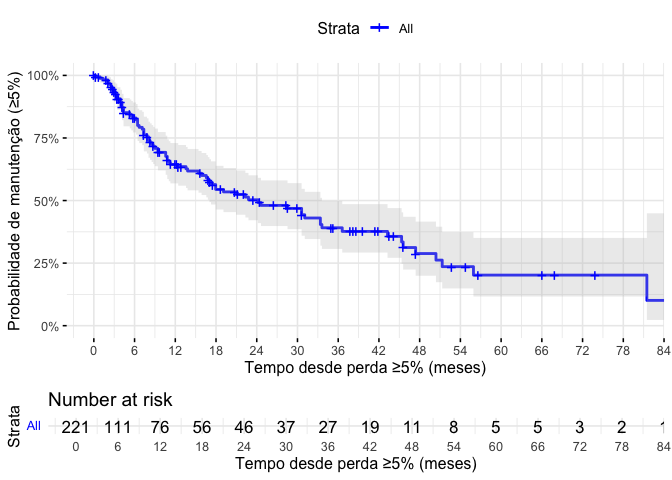
\includegraphics[width=1\textwidth,height=\textheight]{outputs/figs/km-manutencao-5-1.png}

}

\caption{Curva de Kaplan--Meier para manutenção de perda de peso ≥5\% em
relação ao basal.}

\end{figure}%

\begin{quote}
Legenda:\\
A curva de Kaplan--Meier para manutenção da perda ≥5\% mostra uma
probabilidade elevada de sustentar a meta de perda de 5\% nos primeiros
meses após o alcance, com queda progressiva ao longo do seguimento.
Aproximadamente 83\% dos pacientes mantinham a perda em 6 meses e 64\%
em 12 meses. A mediana do tempo até o reganho foi de 24,2 meses,
indicando que metade dos pacientes manteve o benefício clínico por pelo
menos dois anos. A curva evidencia ainda que, embora haja declínio
gradual, uma proporção considerável de indivíduos preservou a perda ≥5\%
até três anos de acompanhamento.\\
\end{quote}

\begin{Shaded}
\begin{Highlighting}[]
\FunctionTok{library}\NormalTok{(dplyr)}
\FunctionTok{library}\NormalTok{(ggplot2)}

\CommentTok{\# manter apenas quem teve evento de reganho (\textless{}5\%)}
\NormalTok{df\_evento }\OtherTok{\textless{}{-}}\NormalTok{ reganho\_primeiro }\SpecialCharTok{\%\textgreater{}\%}
  \FunctionTok{filter}\NormalTok{(event) }\SpecialCharTok{\%\textgreater{}\%}
  \FunctionTok{transmute}\NormalTok{(time\_to\_event\_months)}

\CommentTok{\# calcular a mediana}
\NormalTok{mediana\_val }\OtherTok{\textless{}{-}} \FunctionTok{median}\NormalTok{(df\_evento}\SpecialCharTok{$}\NormalTok{time\_to\_event\_months, }\AttributeTok{na.rm =} \ConstantTok{TRUE}\NormalTok{)}

\NormalTok{mediana\_val}
\end{Highlighting}
\end{Shaded}

\begin{verbatim}
[1] 8.975834
\end{verbatim}

\begin{Shaded}
\begin{Highlighting}[]
\CommentTok{\# gráfico violino + boxplot + pontos + linha de mediana destacada}
\FunctionTok{ggplot}\NormalTok{(df\_evento, }\FunctionTok{aes}\NormalTok{(}\AttributeTok{x =} \StringTok{""}\NormalTok{, }\AttributeTok{y =}\NormalTok{ time\_to\_event\_months)) }\SpecialCharTok{+}
  \FunctionTok{geom\_violin}\NormalTok{(}\AttributeTok{trim =} \ConstantTok{FALSE}\NormalTok{, }\AttributeTok{alpha =} \FloatTok{0.4}\NormalTok{, }\AttributeTok{fill =} \StringTok{"grey80"}\NormalTok{) }\SpecialCharTok{+}
  \FunctionTok{geom\_boxplot}\NormalTok{(}\AttributeTok{width =} \FloatTok{0.15}\NormalTok{, }\AttributeTok{outlier.shape =} \ConstantTok{NA}\NormalTok{, }\AttributeTok{fill =} \StringTok{"white"}\NormalTok{) }\SpecialCharTok{+}
  \FunctionTok{geom\_jitter}\NormalTok{(}\AttributeTok{width =} \FloatTok{0.08}\NormalTok{, }\AttributeTok{alpha =} \FloatTok{0.3}\NormalTok{, }\AttributeTok{size =} \DecValTok{1}\NormalTok{) }\SpecialCharTok{+}
  \FunctionTok{geom\_hline}\NormalTok{(}\AttributeTok{yintercept =}\NormalTok{ mediana\_val, }\AttributeTok{linetype =} \StringTok{"dashed"}\NormalTok{, }\AttributeTok{color =} \StringTok{"red"}\NormalTok{, }\AttributeTok{linewidth =} \DecValTok{1}\NormalTok{) }\SpecialCharTok{+}
  \CommentTok{\#annotate("text", x = 1.2, y = mediana\_val,}
  \CommentTok{\#         label = paste0("Mediana: ", round(mediana\_val, 1), " meses"),}
  \CommentTok{\#         color = "red", hjust = 0) +}
  \FunctionTok{labs}\NormalTok{(}\AttributeTok{x =} \ConstantTok{NULL}\NormalTok{, }\AttributeTok{y =} \StringTok{"Tempo até reganho (meses)"}\NormalTok{) }\SpecialCharTok{+}
  \FunctionTok{theme\_minimal}\NormalTok{(}\AttributeTok{base\_size =} \DecValTok{12}\NormalTok{) }\SpecialCharTok{+}
  \FunctionTok{theme}\NormalTok{(}\AttributeTok{axis.text.x =} \FunctionTok{element\_blank}\NormalTok{())}
\end{Highlighting}
\end{Shaded}

\begin{figure}[H]

{\centering 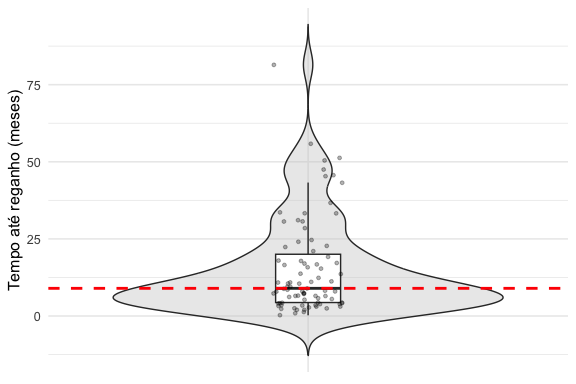
\includegraphics[width=1\textwidth,height=\textheight]{outputs/figs/dist-tempo-ate-reganho-violin-1.png}

}

\caption{Distribuição do tempo até o reganho (\textless5\%) entre quem
atingiu ≥5\%: violino + boxplot.}

\end{figure}%

O código seleciona apenas os pacientes que \textbf{atingiram perda ≥5\%}
e que, em algum momento, \textbf{apresentaram reganho} (definido como
voltar a ter perda \textless5\% em relação ao basal). Em seguida,
calcula a \textbf{mediana do tempo até o primeiro reganho} (em meses)
entre esses pacientes (\texttt{mediana\_val}) e constrói um gráfico
\textbf{violino + boxplot} com pontos individuais para visualizar a
\textbf{distribuição do tempo até o reganho}. A mediana é destacada por
uma \textbf{linha tracejada vermelha} e anotada no gráfico.

\begin{quote}
Legenda:\\
Distribuição do tempo até o primeiro reganho (\textless5\%) entre os
pacientes que atingiram perda ≥5\%. O violino representa a densidade da
distribuição, o boxplot resume a mediana e o intervalo interquartil, e
os pontos mostram observações individuais. A linha tracejada vermelha
destaca a mediana do tempo até o reganho (≈ 9 meses).\\
\end{quote}

\begin{quote}
Resultados:\\
Entre os pacientes que atingiram a meta de perda ≥5\% e posteriormente
apresentaram reganho (queda para \textless5\%), o tempo mediano até o
evento foi de aproximadamente \textbf{9 meses}, com ampla variabilidade
entre indivíduos. Esse resultado contrasta com a estimativa baseada na
análise de sobrevivência de toda a coorte (incluindo censura), na qual a
mediana do tempo até o reganho foi de \textbf{24,2 meses}. Em conjunto,
os achados indicam que, embora uma parcela expressiva mantenha a perda
clinicamente relevante por períodos prolongados, o reganho tende a
ocorrer de forma relativamente precoce entre aqueles suscetíveis.
\end{quote}

\begin{quote}
Discussão - comparação Kaplan-Meier vs.~tempo mediano do evento naqueles
em que o evento de reganho de peso foi observado\\
Entre os pacientes que atingiram perda ≥5\%, o tempo mediano até o
reganho, considerando toda a coorte e incluindo a censura dos indivíduos
que não apresentaram o evento, foi de 24,2 meses (estimado pelo modelo
de Kaplan--Meier). Esse valor indica o ponto em que metade da amostra
ainda mantinha a perda ≥5\%, refletindo a trajetória global do grupo,
inclusive daqueles que nunca perderam o benefício. Por outro lado, ao
analisar apenas os pacientes que efetivamente apresentaram reganho, o
tempo mediano até o evento foi bem menor, cerca de 9 meses (IIQ: 5--18).
Essa segunda métrica revela em quanto tempo, em média, o reganho ocorre
entre os suscetíveis. Em conjunto, os achados mostram que, embora uma
parcela expressiva mantenha a perda clinicamente relevante por períodos
prolongados, o reganho tende a se manifestar precocemente nos indivíduos
vulneráveis.\\
\end{quote}

\begin{Shaded}
\begin{Highlighting}[]
\CommentTok{\# separar tempos de evento e de censura}
\NormalTok{df\_plot }\OtherTok{\textless{}{-}}\NormalTok{ reganho\_primeiro }\SpecialCharTok{\%\textgreater{}\%}
  \FunctionTok{mutate}\NormalTok{(}
    \AttributeTok{tempo\_meses =}\NormalTok{ time\_to\_event\_months,}
    \AttributeTok{status =} \FunctionTok{ifelse}\NormalTok{(event, }\StringTok{"Evento (reganho)"}\NormalTok{, }\StringTok{"Censurado"}\NormalTok{)}
\NormalTok{  )}

\CommentTok{\# histograma para quem teve evento; risquinhos (rug) na base para censurados}
\FunctionTok{ggplot}\NormalTok{() }\SpecialCharTok{+}
  \FunctionTok{geom\_histogram}\NormalTok{(}
    \AttributeTok{data =}\NormalTok{ df\_plot }\SpecialCharTok{\%\textgreater{}\%} \FunctionTok{filter}\NormalTok{(event),}
    \FunctionTok{aes}\NormalTok{(}\AttributeTok{x =}\NormalTok{ tempo\_meses),}
    \AttributeTok{bins =} \DecValTok{18}\NormalTok{,  }\CommentTok{\# \textasciitilde{}classes de 3{-}4 meses, ajuste se desejar}
    \AttributeTok{alpha =} \FloatTok{0.7}
\NormalTok{  ) }\SpecialCharTok{+}
  \FunctionTok{geom\_rug}\NormalTok{(}
    \AttributeTok{data =}\NormalTok{ df\_plot }\SpecialCharTok{\%\textgreater{}\%} \FunctionTok{filter}\NormalTok{(}\SpecialCharTok{!}\NormalTok{event),}
    \FunctionTok{aes}\NormalTok{(}\AttributeTok{x =}\NormalTok{ tempo\_meses),}
    \AttributeTok{sides =} \StringTok{"b"}\NormalTok{,}
    \AttributeTok{alpha =} \FloatTok{0.6}
\NormalTok{  ) }\SpecialCharTok{+}
  \FunctionTok{labs}\NormalTok{(}
    \AttributeTok{x =} \StringTok{"Tempo desde a perda ≥5\% (meses)"}\NormalTok{,}
    \AttributeTok{y =} \StringTok{"Nº de pacientes (com evento)"}\NormalTok{,}
    \AttributeTok{subtitle =} \StringTok{"Barras: eventos de reganho; Rug na base: observações censuradas"}
\NormalTok{  ) }\SpecialCharTok{+}
  \FunctionTok{theme\_minimal}\NormalTok{(}\AttributeTok{base\_size =} \DecValTok{12}\NormalTok{)}
\end{Highlighting}
\end{Shaded}

\begin{figure}[H]

{\centering 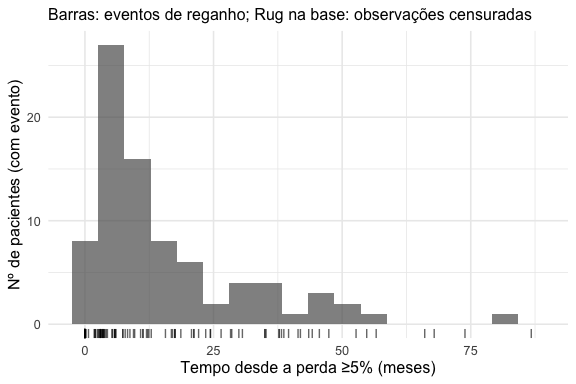
\includegraphics[width=1\textwidth,height=\textheight]{outputs/figs/dist-tempo-ate-reganho-hist-1.png}

}

\caption{Tempo até reganho (\textless5\%): histograma dos eventos e
marcações dos censurados.}

\end{figure}%

O histograma apresenta a distribuição do tempo até o reganho
(\textless5\%) entre os pacientes que atingiram perda ≥5\%. As barras
representam o número de eventos observados em cada intervalo de tempo,
enquanto os traços na base (rug) indicam os tempos de censura, ou seja,
pacientes que não reganharam até a última consulta registrada.

\begin{quote}
Legenda:\\
Distribuição do tempo até o reganho (\textless5\%) entre os pacientes
que atingiram perda ≥5\%. As barras indicam os eventos de reganho e os
traços na base representam os tempos de censura (indivíduos que não
reganharam até a última observação).
\end{quote}

\begin{quote}
Resultados:\\
O histograma dos tempos até o reganho (\textless5\%) mostra maior
concentração de eventos nos primeiros 12 a 18 meses após atingir a meta,
mas também ocorrência esporádica ao longo de períodos mais prolongados.
Os traços na base indicam o seguimento dos pacientes que permaneceram
censurados, evidenciando que parte deles manteve a perda ≥5\% por até
5--6 anos sem apresentar reganho.
\end{quote}

\subsubsection{3.3. No subgrupo com perda ≥5\%, comparar o momento (≤6
meses, 6--12 meses, \textgreater12 meses) em que a meta de perda de 5\%
foi
alcançada.}\label{no-subgrupo-com-perda-5-comparar-o-momento-6-meses-612-meses-12-meses-em-que-a-meta-de-perda-de-5-foi-alcanuxe7ada.}

Objetivo: qual o tempo ideial de seguimento em que (dentre os que
tiveram perda significativa) os indivíduos tem maior probabilidade de
atingir a perda significativa.

Racional: Otimizar o fluxo do ambulatório e definir um tempo ideal para
darmos alta para o paciente, caso ele não atinja a perda de 5\% do peso,
para podermos atender outro caso novo no lugar, dando chance a outra
pessoa de perder peso

\begin{Shaded}
\begin{Highlighting}[]
\DocumentationTok{\#\#\# 3.3. No subgrupo com perda ≥5\%, comparar o momento (≤6m, 6–12m, 12–18m, 18–24m, 24–30m, 30–36m, \textgreater{}36m)}
\DocumentationTok{\#\#\# em que a meta foi alcançada}

\FunctionTok{library}\NormalTok{(dplyr)}
\FunctionTok{library}\NormalTok{(purrr)}

\CommentTok{\# Partimos de \textasciigrave{}momento\_perda5\textasciigrave{} (uma linha por paciente que atingiu ≥5\%)}
\CommentTok{\# Criar meses até a 1ª vez que atingiu ≥5\% e classificar em 7 janelas}
\NormalTok{atingiu\_por\_janela }\OtherTok{\textless{}{-}}\NormalTok{ momento\_perda5 }\SpecialCharTok{\%\textgreater{}\%}
  \FunctionTok{mutate}\NormalTok{(}
    \AttributeTok{meses\_ate\_5 =}\NormalTok{ week\_consultation }\SpecialCharTok{/} \FloatTok{4.345}\NormalTok{,}
    \AttributeTok{janela =} \FunctionTok{case\_when}\NormalTok{(}
\NormalTok{      meses\_ate\_5 }\SpecialCharTok{\textless{}=} \DecValTok{6}                       \SpecialCharTok{\textasciitilde{}} \StringTok{"≤6m"}\NormalTok{,}
\NormalTok{      meses\_ate\_5 }\SpecialCharTok{\textgreater{}} \DecValTok{6}   \SpecialCharTok{\&}\NormalTok{ meses\_ate\_5 }\SpecialCharTok{\textless{}=} \DecValTok{12}  \SpecialCharTok{\textasciitilde{}} \StringTok{"6–12m"}\NormalTok{,}
\NormalTok{      meses\_ate\_5 }\SpecialCharTok{\textgreater{}} \DecValTok{12}  \SpecialCharTok{\&}\NormalTok{ meses\_ate\_5 }\SpecialCharTok{\textless{}=} \DecValTok{18}  \SpecialCharTok{\textasciitilde{}} \StringTok{"12–18m"}\NormalTok{,}
\NormalTok{      meses\_ate\_5 }\SpecialCharTok{\textgreater{}} \DecValTok{18}  \SpecialCharTok{\&}\NormalTok{ meses\_ate\_5 }\SpecialCharTok{\textless{}=} \DecValTok{24}  \SpecialCharTok{\textasciitilde{}} \StringTok{"18–24m"}\NormalTok{,}
\NormalTok{      meses\_ate\_5 }\SpecialCharTok{\textgreater{}} \DecValTok{24}  \SpecialCharTok{\&}\NormalTok{ meses\_ate\_5 }\SpecialCharTok{\textless{}=} \DecValTok{30}  \SpecialCharTok{\textasciitilde{}} \StringTok{"24–30m"}\NormalTok{,}
\NormalTok{      meses\_ate\_5 }\SpecialCharTok{\textgreater{}} \DecValTok{30}  \SpecialCharTok{\&}\NormalTok{ meses\_ate\_5 }\SpecialCharTok{\textless{}=} \DecValTok{36}  \SpecialCharTok{\textasciitilde{}} \StringTok{"30–36m"}\NormalTok{,}
\NormalTok{      meses\_ate\_5 }\SpecialCharTok{\textgreater{}} \DecValTok{36}                       \SpecialCharTok{\textasciitilde{}} \StringTok{"\textgreater{}36m"}\NormalTok{,}
      \ConstantTok{TRUE} \SpecialCharTok{\textasciitilde{}} \ConstantTok{NA\_character\_}
\NormalTok{    ),}
    \AttributeTok{janela =} \FunctionTok{factor}\NormalTok{(janela,}
                    \AttributeTok{levels =} \FunctionTok{c}\NormalTok{(}\StringTok{"≤6m"}\NormalTok{,}\StringTok{"6–12m"}\NormalTok{,}\StringTok{"12–18m"}\NormalTok{,}
                               \StringTok{"18–24m"}\NormalTok{,}\StringTok{"24–30m"}\NormalTok{,}\StringTok{"30–36m"}\NormalTok{,}\StringTok{"\textgreater{}36m"}\NormalTok{))}
\NormalTok{  ) }\SpecialCharTok{\%\textgreater{}\%}
  \FunctionTok{filter}\NormalTok{(}\SpecialCharTok{!}\FunctionTok{is.na}\NormalTok{(janela))}

\CommentTok{\# Resumo com IC95\% binomial para a proporção em cada janela}
\NormalTok{resumo\_janelas }\OtherTok{\textless{}{-}}\NormalTok{ atingiu\_por\_janela }\SpecialCharTok{\%\textgreater{}\%}
  \FunctionTok{count}\NormalTok{(janela, }\AttributeTok{name =} \StringTok{"n"}\NormalTok{) }\SpecialCharTok{\%\textgreater{}\%}
  \FunctionTok{mutate}\NormalTok{(}
    \AttributeTok{N\_total =} \FunctionTok{sum}\NormalTok{(n),}
    \AttributeTok{prop    =}\NormalTok{ n }\SpecialCharTok{/}\NormalTok{ N\_total}
\NormalTok{  ) }\SpecialCharTok{\%\textgreater{}\%}
  \FunctionTok{rowwise}\NormalTok{() }\SpecialCharTok{\%\textgreater{}\%}
  \FunctionTok{mutate}\NormalTok{(}
    \AttributeTok{ci\_low  =} \FunctionTok{binom.test}\NormalTok{(n, N\_total)}\SpecialCharTok{$}\NormalTok{conf.int[}\DecValTok{1}\NormalTok{],}
    \AttributeTok{ci\_high =} \FunctionTok{binom.test}\NormalTok{(n, N\_total)}\SpecialCharTok{$}\NormalTok{conf.int[}\DecValTok{2}\NormalTok{]}
\NormalTok{  ) }\SpecialCharTok{\%\textgreater{}\%}
  \FunctionTok{ungroup}\NormalTok{()}

\NormalTok{knitr}\SpecialCharTok{::}\FunctionTok{kable}\NormalTok{(}
\NormalTok{  resumo\_janelas,}
  \AttributeTok{digits =} \DecValTok{3}\NormalTok{,}
  \AttributeTok{col.names =} \FunctionTok{c}\NormalTok{(}\StringTok{"Janela"}\NormalTok{, }\StringTok{"n"}\NormalTok{, }\StringTok{"N total"}\NormalTok{, }\StringTok{"Proporção"}\NormalTok{, }\StringTok{"IC95\% inferior"}\NormalTok{, }\StringTok{"IC95\% superior"}\NormalTok{),}
  \AttributeTok{caption =} \StringTok{"Distribuição do primeiro alcance de perda ≥5\% por janela de tempo entre os que atingiram a meta."}\NormalTok{,}
  \AttributeTok{align =} \FunctionTok{c}\NormalTok{(}\StringTok{"l"}\NormalTok{, }\StringTok{"c"}\NormalTok{, }\StringTok{"c"}\NormalTok{, }\StringTok{"c"}\NormalTok{, }\StringTok{"c"}\NormalTok{, }\StringTok{"c"}\NormalTok{)}
\NormalTok{)}
\end{Highlighting}
\end{Shaded}

\begin{longtable}[]{@{}lccccc@{}}
\caption{Distribuição do primeiro alcance de perda ≥5\% por janela de
tempo entre os que atingiram a meta.}\tabularnewline
\toprule\noalign{}
Janela & n & N total & Proporção & IC95\% inferior & IC95\% superior \\
\midrule\noalign{}
\endfirsthead
\toprule\noalign{}
Janela & n & N total & Proporção & IC95\% inferior & IC95\% superior \\
\midrule\noalign{}
\endhead
\bottomrule\noalign{}
\endlastfoot
≤6m & 67 & 221 & 0.303 & 0.243 & 0.368 \\
6--12m & 63 & 221 & 0.285 & 0.227 & 0.349 \\
12--18m & 29 & 221 & 0.131 & 0.090 & 0.183 \\
18--24m & 16 & 221 & 0.072 & 0.042 & 0.115 \\
24--30m & 10 & 221 & 0.045 & 0.022 & 0.082 \\
30--36m & 8 & 221 & 0.036 & 0.016 & 0.070 \\
\textgreater36m & 28 & 221 & 0.127 & 0.086 & 0.178 \\
\end{longtable}

Esse código agora cria sete categorias de tempo (≤6m, 6--12m, 12--18m,
18--24m, 24--30m, 30--36m, \textgreater36m) para identificar em qual
janela os pacientes que atingiram ≥5\% chegaram à meta. A tabela
resumo\_janelas mostra n, proporção e IC95\% em cada faixa.

\begin{quote}
Interpretação:\\
Entre os \textbf{221 pacientes que atingiram perda ≥5\%}, a distribuição
do \textbf{primeiro alcance} da meta ocorreu de forma heterogênea ao
longo do seguimento:\\
\strut \\
- \textbf{≤6 meses:} 30,3\% (IC95\%: 24,3--36,8)\\
- \textbf{6--12 meses:} 28,5\% (IC95\%: 22,7--34,9)\\
- \textbf{12--18 meses:} 13,1\% (IC95\%: 9,0--18,3)\\
- \textbf{18--24 meses:} 7,2\% (IC95\%: 4,2--11,5)\\
- \textbf{24--30 meses:} 4,5\% (IC95\%: 2,2--8,2)\\
- \textbf{30--36 meses:} 3,6\% (IC95\%: 1,6--7,0)\\
- \textbf{\textgreater36 meses:} 12,7\% (IC95\%: 8,6--17,8)\\
\end{quote}

\begin{quote}
Resultados:\\
Mais da metade dos pacientes respondeu em até \textbf{12 meses}
(58,8\%), com maior concentração nos primeiros 6 meses (30,3\%).
Entretanto, uma proporção não desprezível (≈41,2\%) atingiu a meta após
12 meses, incluindo 12,7\% somente após 36 meses de seguimento.\\
\end{quote}

\begin{quote}
Discussão:~ Esses achados sugerem que, embora o período de \textbf{até
12 meses} seja o mais produtivo para identificar respondedores precoces,
ainda há uma parcela significativa de \textbf{respondedores tardios} que
podem se beneficiar de um seguimento prolongado. Do ponto de vista
clínico e de gestão ambulatorial, isso sugere que uma \textbf{alta
precoce baseada apenas na ausência de resposta em 12 meses} poderia
descartar pacientes com chance real de atingir benefício clínico
relevante em períodos posteriores.\\
\end{quote}

\begin{Shaded}
\begin{Highlighting}[]
\FunctionTok{library}\NormalTok{(ggplot2)}
\FunctionTok{library}\NormalTok{(scales)}
\FunctionTok{library}\NormalTok{(dplyr)}

\CommentTok{\# garantir ordem e colunas auxiliares para rótulos (\% e n)}
\NormalTok{plot\_janelas }\OtherTok{\textless{}{-}}\NormalTok{ resumo\_janelas }\SpecialCharTok{\%\textgreater{}\%}
  \FunctionTok{mutate}\NormalTok{(}
    \AttributeTok{janela =} \FunctionTok{factor}\NormalTok{(janela,}
      \AttributeTok{levels =} \FunctionTok{c}\NormalTok{(}\StringTok{"≤6m"}\NormalTok{,}\StringTok{"6–12m"}\NormalTok{,}\StringTok{"12–18m"}\NormalTok{,}\StringTok{"18–24m"}\NormalTok{,}\StringTok{"24–30m"}\NormalTok{,}\StringTok{"30–36m"}\NormalTok{,}\StringTok{"\textgreater{}36m"}\NormalTok{)}
\NormalTok{    ),}
    \AttributeTok{prop\_lab =} \FunctionTok{percent}\NormalTok{(prop, }\AttributeTok{accuracy =} \FloatTok{0.1}\NormalTok{),}
    \AttributeTok{n\_lab =} \FunctionTok{paste0}\NormalTok{(}\StringTok{"n="}\NormalTok{, n)}
\NormalTok{  )}

\FunctionTok{ggplot}\NormalTok{(plot\_janelas, }\FunctionTok{aes}\NormalTok{(}\AttributeTok{x =}\NormalTok{ janela, }\AttributeTok{y =}\NormalTok{ prop)) }\SpecialCharTok{+}
  \FunctionTok{geom\_col}\NormalTok{(}\AttributeTok{width =} \FloatTok{0.7}\NormalTok{) }\SpecialCharTok{+}
  \FunctionTok{geom\_errorbar}\NormalTok{(}\FunctionTok{aes}\NormalTok{(}\AttributeTok{ymin =}\NormalTok{ ci\_low, }\AttributeTok{ymax =}\NormalTok{ ci\_high), }\AttributeTok{width =} \FloatTok{0.12}\NormalTok{, }\AttributeTok{linewidth =} \FloatTok{0.7}\NormalTok{) }\SpecialCharTok{+}
  \FunctionTok{geom\_text}\NormalTok{(}\FunctionTok{aes}\NormalTok{(}\AttributeTok{label =}\NormalTok{ prop\_lab), }\AttributeTok{vjust =} \SpecialCharTok{{-}}\FloatTok{0.4}\NormalTok{, }\AttributeTok{size =} \FloatTok{3.3}\NormalTok{) }\SpecialCharTok{+}
  \FunctionTok{geom\_text}\NormalTok{(}\FunctionTok{aes}\NormalTok{(}\AttributeTok{label =}\NormalTok{ n\_lab, }\AttributeTok{y =} \FunctionTok{pmax}\NormalTok{(prop }\SpecialCharTok{{-}} \FloatTok{0.04}\NormalTok{, }\FloatTok{0.01}\NormalTok{)), }\CommentTok{\# rótulo de n dentro da barra}
            \AttributeTok{color =} \StringTok{"white"}\NormalTok{, }\AttributeTok{fontface =} \StringTok{"bold"}\NormalTok{, }\AttributeTok{size =} \DecValTok{3}\NormalTok{) }\SpecialCharTok{+}
  \FunctionTok{scale\_y\_continuous}\NormalTok{(}\AttributeTok{labels =} \FunctionTok{percent\_format}\NormalTok{(}\AttributeTok{accuracy =} \DecValTok{1}\NormalTok{), }\AttributeTok{limits =} \FunctionTok{c}\NormalTok{(}\DecValTok{0}\NormalTok{, }\FloatTok{0.4}\NormalTok{)) }\SpecialCharTok{+}
  \FunctionTok{labs}\NormalTok{(}\AttributeTok{x =} \StringTok{"Janela da 1ª vez que atingiu ≥5\%"}\NormalTok{, }\AttributeTok{y =} \StringTok{"Proporção dos respondedores (\%)"}\NormalTok{) }\SpecialCharTok{+}
  \FunctionTok{theme\_minimal}\NormalTok{(}\AttributeTok{base\_size =} \DecValTok{12}\NormalTok{) }\SpecialCharTok{+}
  \FunctionTok{theme}\NormalTok{(}
    \AttributeTok{panel.grid.minor =} \FunctionTok{element\_blank}\NormalTok{(),}
    \AttributeTok{axis.title.x =} \FunctionTok{element\_text}\NormalTok{(}\AttributeTok{margin =} \FunctionTok{margin}\NormalTok{(}\AttributeTok{t =} \DecValTok{8}\NormalTok{)),}
    \AttributeTok{axis.title.y =} \FunctionTok{element\_text}\NormalTok{(}\AttributeTok{margin =} \FunctionTok{margin}\NormalTok{(}\AttributeTok{r =} \DecValTok{8}\NormalTok{))}
\NormalTok{  )}
\end{Highlighting}
\end{Shaded}

\begin{figure}[H]

{\centering 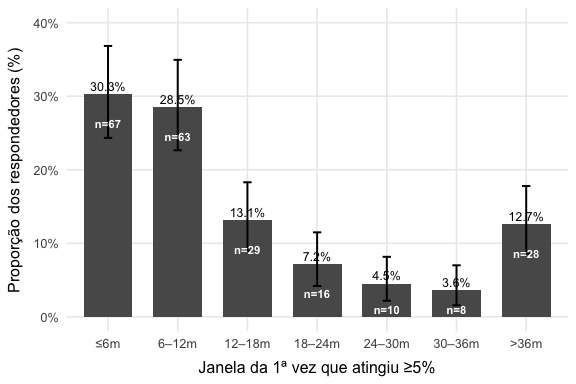
\includegraphics[width=1\textwidth,height=\textheight]{outputs/figs/grafico-atingiu-por-janela-1.png}

}

\caption{Distribuição do primeiro alcance de perda ≥5\% por janela de
tempo entre os que atingiram a meta (proporção e IC95\%).}

\end{figure}%

\begin{quote}
Legenda:\\
Distribuição do primeiro alcance de perda ≥5\% por janelas de tempo
entre os pacientes que atingiram a meta. As barras representam a
proporção (\%) de respondedores em cada intervalo, com intervalos de
confiança de 95\%. Os valores sobre as colunas indicam a proporção e o
número absoluto de pacientes (n) em cada grupo.
\end{quote}

\subsubsection{Probabilidade cumulativa de atingir
≥5\%}\label{probabilidade-cumulativa-de-atingir-5}

\begin{Shaded}
\begin{Highlighting}[]
\CommentTok{\# Probabilidade cumulativa de atingir ≥5\% em múltiplos tempos (≤6m, 6–12m, 12–18m, 18–24m, 24–30m, 30–36m)}
\CommentTok{\# Evento = "atingir ≥5\%"; censura = não atingiu até a última consulta}

\FunctionTok{library}\NormalTok{(dplyr)}
\FunctionTok{library}\NormalTok{(survival)}
\FunctionTok{library}\NormalTok{(tibble)}

\CommentTok{\# 1) Construir objeto de tempo para TODA a coorte (inclui quem nunca atingiu)}
\NormalTok{tempo\_evento }\OtherTok{\textless{}{-}}\NormalTok{ momento\_perda5 }\SpecialCharTok{\%\textgreater{}\%}
  \FunctionTok{transmute}\NormalTok{(record\_id, }\AttributeTok{t\_event\_meses =}\NormalTok{ week\_consultation }\SpecialCharTok{/} \FloatTok{4.345}\NormalTok{, }\AttributeTok{status =} \DecValTok{1}\NormalTok{)}

\NormalTok{tempo\_cens }\OtherTok{\textless{}{-}}\NormalTok{ obese }\SpecialCharTok{\%\textgreater{}\%}
  \FunctionTok{group\_by}\NormalTok{(record\_id) }\SpecialCharTok{\%\textgreater{}\%}
  \FunctionTok{summarize}\NormalTok{(}\AttributeTok{t\_last\_meses =} \FunctionTok{max}\NormalTok{(week\_consultation, }\AttributeTok{na.rm =} \ConstantTok{TRUE}\NormalTok{) }\SpecialCharTok{/} \FloatTok{4.345}\NormalTok{, }\AttributeTok{.groups =} \StringTok{"drop"}\NormalTok{)}

\NormalTok{coorte\_tempo }\OtherTok{\textless{}{-}}\NormalTok{ tempo\_cens }\SpecialCharTok{\%\textgreater{}\%}
  \FunctionTok{left\_join}\NormalTok{(tempo\_evento, }\AttributeTok{by =} \StringTok{"record\_id"}\NormalTok{) }\SpecialCharTok{\%\textgreater{}\%}
  \FunctionTok{mutate}\NormalTok{(}
    \AttributeTok{time   =} \FunctionTok{ifelse}\NormalTok{(}\SpecialCharTok{!}\FunctionTok{is.na}\NormalTok{(t\_event\_meses), t\_event\_meses, t\_last\_meses),}
    \AttributeTok{status =} \FunctionTok{ifelse}\NormalTok{(}\SpecialCharTok{!}\FunctionTok{is.na}\NormalTok{(t\_event\_meses), }\DecValTok{1}\NormalTok{, }\DecValTok{0}\NormalTok{)  }\CommentTok{\# 1 = atingiu; 0 = censurado}
\NormalTok{  )}

\CommentTok{\# 2) Ajustar KM (sobrevida = ainda NÃO atingiu). Cumulativa = 1 {-} S(t)}
\NormalTok{fit\_atingir }\OtherTok{\textless{}{-}} \FunctionTok{survfit}\NormalTok{(}\FunctionTok{Surv}\NormalTok{(time, status) }\SpecialCharTok{\textasciitilde{}} \DecValTok{1}\NormalTok{, }\AttributeTok{data =}\NormalTok{ coorte\_tempo, }\AttributeTok{conf.type =} \StringTok{"log"}\NormalTok{)}

\CommentTok{\# 3) Tempos{-}alvo (em meses)}
\NormalTok{tempos\_alvo }\OtherTok{\textless{}{-}} \FunctionTok{c}\NormalTok{(}\DecValTok{6}\NormalTok{, }\DecValTok{12}\NormalTok{, }\DecValTok{18}\NormalTok{, }\DecValTok{24}\NormalTok{, }\DecValTok{30}\NormalTok{, }\DecValTok{36}\NormalTok{)}

\CommentTok{\# 4) Extrair S(t) e IC95\% e converter para probabilidade cumulativa 1 {-} S(t)}
\NormalTok{sum\_atingir }\OtherTok{\textless{}{-}} \FunctionTok{summary}\NormalTok{(fit\_atingir, }\AttributeTok{times =}\NormalTok{ tempos\_alvo, }\AttributeTok{extend =} \ConstantTok{TRUE}\NormalTok{)}

\NormalTok{tabela\_cuminc }\OtherTok{\textless{}{-}} \FunctionTok{tibble}\NormalTok{(}
  \AttributeTok{tempo\_meses =}\NormalTok{ sum\_atingir}\SpecialCharTok{$}\NormalTok{time,}
  \AttributeTok{prob\_atingir =} \DecValTok{1} \SpecialCharTok{{-}}\NormalTok{ sum\_atingir}\SpecialCharTok{$}\NormalTok{surv,         }\CommentTok{\# cumulativa}
  \AttributeTok{ic\_low       =} \DecValTok{1} \SpecialCharTok{{-}}\NormalTok{ sum\_atingir}\SpecialCharTok{$}\NormalTok{upper,        }\CommentTok{\# inverter limites de S(t)}
  \AttributeTok{ic\_high      =} \DecValTok{1} \SpecialCharTok{{-}}\NormalTok{ sum\_atingir}\SpecialCharTok{$}\NormalTok{lower}
\NormalTok{)}

\CommentTok{\# Tabela formatada (percentuais) para o artigo}
\NormalTok{tabela\_cuminc\_fmt }\OtherTok{\textless{}{-}}\NormalTok{ tabela\_cuminc }\SpecialCharTok{\%\textgreater{}\%}
  \FunctionTok{mutate}\NormalTok{(}
    \StringTok{\textasciigrave{}}\AttributeTok{Prob (\%)}\StringTok{\textasciigrave{}} \OtherTok{=}\NormalTok{ prob\_atingir }\SpecialCharTok{*} \DecValTok{100}\NormalTok{,}
    \StringTok{\textasciigrave{}}\AttributeTok{IC95\% inferior}\StringTok{\textasciigrave{}} \OtherTok{=}\NormalTok{ ic\_low }\SpecialCharTok{*} \DecValTok{100}\NormalTok{,}
    \StringTok{\textasciigrave{}}\AttributeTok{IC95\% superior}\StringTok{\textasciigrave{}} \OtherTok{=}\NormalTok{ ic\_high }\SpecialCharTok{*} \DecValTok{100}
\NormalTok{  ) }\SpecialCharTok{\%\textgreater{}\%}
  \FunctionTok{select}\NormalTok{(}\StringTok{\textasciigrave{}}\AttributeTok{Tempo (meses)}\StringTok{\textasciigrave{}} \OtherTok{=}\NormalTok{ tempo\_meses, }\StringTok{\textasciigrave{}}\AttributeTok{Prob (\%)}\StringTok{\textasciigrave{}}\NormalTok{, }\StringTok{\textasciigrave{}}\AttributeTok{IC95\% inferior}\StringTok{\textasciigrave{}}\NormalTok{, }\StringTok{\textasciigrave{}}\AttributeTok{IC95\% superior}\StringTok{\textasciigrave{}}\NormalTok{)}

\NormalTok{knitr}\SpecialCharTok{::}\FunctionTok{kable}\NormalTok{(}
\NormalTok{  tabela\_cuminc\_fmt,}
  \AttributeTok{digits =} \DecValTok{3}\NormalTok{,}
  \AttributeTok{caption =} \StringTok{"Probabilidade cumulativa de atingir perda ≥5\% em múltiplos tempos após o início do acompanhamento."}\NormalTok{,}
  \AttributeTok{align =} \FunctionTok{c}\NormalTok{(}\StringTok{"c"}\NormalTok{, }\StringTok{"c"}\NormalTok{, }\StringTok{"c"}\NormalTok{, }\StringTok{"c"}\NormalTok{)}
\NormalTok{)}
\end{Highlighting}
\end{Shaded}

\begin{longtable}[]{@{}cccc@{}}
\caption{Probabilidade cumulativa de atingir perda ≥5\% em múltiplos
tempos após o início do acompanhamento.}\tabularnewline
\toprule\noalign{}
Tempo (meses) & Prob (\%) & IC95\% inferior & IC95\% superior \\
\midrule\noalign{}
\endfirsthead
\toprule\noalign{}
Tempo (meses) & Prob (\%) & IC95\% inferior & IC95\% superior \\
\midrule\noalign{}
\endhead
\bottomrule\noalign{}
\endlastfoot
6 & 12.760 & 9.849 & 15.577 \\
12 & 27.603 & 23.369 & 31.604 \\
18 & 36.008 & 31.192 & 40.487 \\
24 & 41.483 & 36.302 & 46.243 \\
30 & 45.632 & 40.131 & 50.627 \\
36 & 49.756 & 43.864 & 55.029 \\
\end{longtable}

Esse chunk calcula, para toda a coorte com censura, a probabilidade
cumulativa de atingir ≥5\% em 6, 12, 18, 24, 30 e 36 meses, com IC95\%
(Greenwood via survfit). O argumento extend = TRUE mantém o último valor
de S(t) caso o tempo solicitado ultrapasse o último tempo observado.

\begin{quote}
Resultados:\\
Na análise de tempo até evento com censura (Kaplan--Meier), a
probabilidade cumulativa de atingir perda ≥5\% aumentou progressivamente
ao longo do seguimento. Aos 6 meses, cerca de 12,8\% (IC95\%: 9,8--15,6)
dos pacientes já haviam alcançado a meta. Esse percentual subiu para
27,6\% (IC95\%: 23,4--31,6) aos 12 meses, 36,0\% (IC95\%: 31,2--40,5)
aos 18 meses, e 41,5\% (IC95\%: 36,3--46,2) aos 24 meses.\\
No seguimento mais prolongado, as chances continuaram a crescer,
atingindo 45,6\% (IC95\%: 40,1--50,6) aos 30 meses\\
e 49,8\% (IC95\%: 43,9--55,0) aos 36 meses de acompanhamento.\\
Interpretação: aproximadamente metade da coorte atingiu perda ≥5\% até
três anos de seguimento. O maior ganho em probabilidade ocorreu nos
primeiros 12 meses, mas uma fração importante de pacientes ainda atingiu
a meta após esse período, reforçando a relevância do acompanhamento
prolongado.\\
\end{quote}

\begin{Shaded}
\begin{Highlighting}[]
\FunctionTok{library}\NormalTok{(ggplot2)}
\FunctionTok{library}\NormalTok{(scales)}

\CommentTok{\# Curva KM como 1 {-} S(t) (suavizado em degraus) + pontos com IC95\% nos marcos}
\CommentTok{\# Construir data.frame da curva cumulativa completa}
\NormalTok{km\_step }\OtherTok{\textless{}{-}} \FunctionTok{data.frame}\NormalTok{(}
  \AttributeTok{time =}\NormalTok{ fit\_atingir}\SpecialCharTok{$}\NormalTok{time,}
  \AttributeTok{cuminc =} \DecValTok{1} \SpecialCharTok{{-}}\NormalTok{ fit\_atingir}\SpecialCharTok{$}\NormalTok{surv}
\NormalTok{)}

\FunctionTok{ggplot}\NormalTok{(km\_step, }\FunctionTok{aes}\NormalTok{(}\AttributeTok{x =}\NormalTok{ time, }\AttributeTok{y =}\NormalTok{ cuminc)) }\SpecialCharTok{+}
  \FunctionTok{geom\_step}\NormalTok{(}\AttributeTok{linewidth =} \FloatTok{0.9}\NormalTok{) }\SpecialCharTok{+}
  \FunctionTok{geom\_point}\NormalTok{(}\AttributeTok{data =}\NormalTok{ tabela\_cuminc,}
             \FunctionTok{aes}\NormalTok{(}\AttributeTok{x =}\NormalTok{ tempo\_meses, }\AttributeTok{y =}\NormalTok{ prob\_atingir)) }\SpecialCharTok{+}
  \FunctionTok{geom\_errorbar}\NormalTok{(}\AttributeTok{data =}\NormalTok{ tabela\_cuminc,}
                \FunctionTok{aes}\NormalTok{(}\AttributeTok{x =}\NormalTok{ tempo\_meses, }\AttributeTok{ymin =}\NormalTok{ ic\_low, }\AttributeTok{ymax =}\NormalTok{ ic\_high),}
                \AttributeTok{width =} \FloatTok{0.6}\NormalTok{, }\AttributeTok{linewidth =} \FloatTok{0.6}\NormalTok{, }\AttributeTok{inherit.aes =} \ConstantTok{FALSE}\NormalTok{) }\SpecialCharTok{+}
  \FunctionTok{scale\_y\_continuous}\NormalTok{(}\AttributeTok{labels =} \FunctionTok{percent\_format}\NormalTok{(}\AttributeTok{accuracy =} \DecValTok{1}\NormalTok{), }\AttributeTok{limits =} \FunctionTok{c}\NormalTok{(}\DecValTok{0}\NormalTok{, }\DecValTok{1}\NormalTok{)) }\SpecialCharTok{+}
  \FunctionTok{scale\_x\_continuous}\NormalTok{(}\AttributeTok{breaks =}\NormalTok{ tempos\_alvo) }\SpecialCharTok{+}
  \FunctionTok{labs}\NormalTok{(}\AttributeTok{x =} \StringTok{"Tempo (meses)"}\NormalTok{, }\AttributeTok{y =} \StringTok{"Probabilidade cumulativa (atingir ≥5\%)"}\NormalTok{) }\SpecialCharTok{+}
  \FunctionTok{theme\_minimal}\NormalTok{(}\AttributeTok{base\_size =} \DecValTok{12}\NormalTok{)}
\end{Highlighting}
\end{Shaded}

\begin{figure}[H]

{\centering 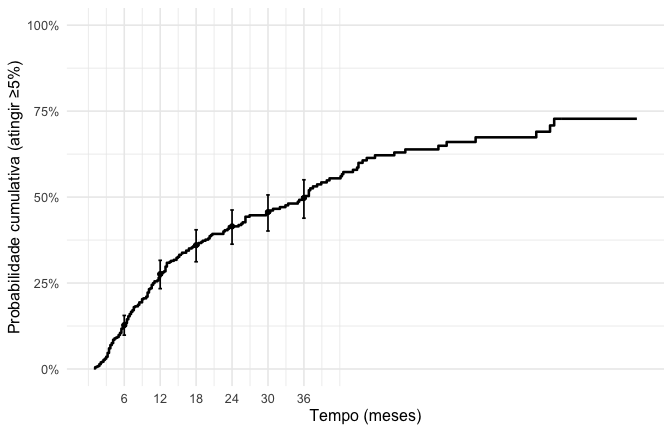
\includegraphics[width=1\textwidth,height=\textheight]{outputs/figs/plot-cuminc-atingir-5-varias-janelas-1.png}

}

\caption{Probabilidade cumulativa de atingir perda ≥5\% (evento) ao
longo do tempo, com IC95\% nos marcos de 6, 12, 18, 24, 30 e 36 meses.}

\end{figure}%

O gráfico mostra a curva cumulativa (1 − S(t)) e destaca, com pontos e
IC95\%, os marcos de 6, 12, 18, 24, 30 e 36 meses. Assim, você visualiza
tanto a evolução contínua quanto os pontos de decisão úteis para o fluxo
ambulatorial.

\begin{quote}
Legenda:\\
Curva de Kaplan--Meier mostrando a probabilidade cumulativa de atingir
perda ≥5\% ao longo do tempo, considerando a censura dos pacientes que
não alcançaram o evento. Os pontos pretos na curva indicam os marcos de
6, 12, 18, 24, 30 e 36 meses, com seus respectivos intervalos de
confiança de 95\%, evidenciando a progressão contínua da proporção de
pacientes que atingiram a meta durante o seguimento.
\end{quote}

\subsubsection{Probabilidade condicional de atingir ≥5\% em janelas
sucessivas, dado que ainda não atingiu no início da
janela}\label{probabilidade-condicional-de-atingir-5-em-janelas-sucessivas-dado-que-ainda-nuxe3o-atingiu-no-inuxedcio-da-janela}

\begin{Shaded}
\begin{Highlighting}[]
\CommentTok{\# Objetivo: estimar probabilidades CONDICIONAIS por janelas sucessivas:}
\CommentTok{\# P(atingir ≥5\% em (a,b] | ainda não atingiu até a)}
\CommentTok{\# a partir da curva de sobrevivência (KM) para "tempo até atingir ≥5\%".}

\FunctionTok{library}\NormalTok{(dplyr)}
\FunctionTok{library}\NormalTok{(survival)}
\FunctionTok{library}\NormalTok{(tibble)}
\FunctionTok{library}\NormalTok{(ggplot2)}
\FunctionTok{library}\NormalTok{(scales)}

\CommentTok{\# {-}{-}{-} (re)construir objeto de tempo da coorte inteira (evento = atingir ≥5\%) {-}{-}{-}}
\NormalTok{tempo\_evento }\OtherTok{\textless{}{-}}\NormalTok{ momento\_perda5 }\SpecialCharTok{\%\textgreater{}\%}
  \FunctionTok{transmute}\NormalTok{(record\_id, }\AttributeTok{t\_event\_meses =}\NormalTok{ week\_consultation }\SpecialCharTok{/} \FloatTok{4.345}\NormalTok{, }\AttributeTok{status =} \DecValTok{1}\NormalTok{)}

\NormalTok{tempo\_cens }\OtherTok{\textless{}{-}}\NormalTok{ obese }\SpecialCharTok{\%\textgreater{}\%}
  \FunctionTok{group\_by}\NormalTok{(record\_id) }\SpecialCharTok{\%\textgreater{}\%}
  \FunctionTok{summarize}\NormalTok{(}\AttributeTok{t\_last\_meses =} \FunctionTok{max}\NormalTok{(week\_consultation, }\AttributeTok{na.rm =} \ConstantTok{TRUE}\NormalTok{) }\SpecialCharTok{/} \FloatTok{4.345}\NormalTok{, }\AttributeTok{.groups =} \StringTok{"drop"}\NormalTok{)}

\NormalTok{coorte\_tempo }\OtherTok{\textless{}{-}}\NormalTok{ tempo\_cens }\SpecialCharTok{\%\textgreater{}\%}
  \FunctionTok{left\_join}\NormalTok{(tempo\_evento, }\AttributeTok{by =} \StringTok{"record\_id"}\NormalTok{) }\SpecialCharTok{\%\textgreater{}\%}
  \FunctionTok{mutate}\NormalTok{(}
    \AttributeTok{time   =} \FunctionTok{ifelse}\NormalTok{(}\SpecialCharTok{!}\FunctionTok{is.na}\NormalTok{(t\_event\_meses), t\_event\_meses, t\_last\_meses),}
    \AttributeTok{status =} \FunctionTok{ifelse}\NormalTok{(}\SpecialCharTok{!}\FunctionTok{is.na}\NormalTok{(t\_event\_meses), }\DecValTok{1}\NormalTok{, }\DecValTok{0}\NormalTok{)  }\CommentTok{\# 1 = atingiu; 0 = censurado}
\NormalTok{  )}

\NormalTok{fit\_atingir }\OtherTok{\textless{}{-}} \FunctionTok{survfit}\NormalTok{(}\FunctionTok{Surv}\NormalTok{(time, status) }\SpecialCharTok{\textasciitilde{}} \DecValTok{1}\NormalTok{, }\AttributeTok{data =}\NormalTok{ coorte\_tempo, }\AttributeTok{conf.type =} \StringTok{"log"}\NormalTok{)}

\CommentTok{\# {-}{-}{-} Janelas desejadas (em meses) {-}{-}{-}}
\CommentTok{\# vamos calcular P((0,6] | T\textgreater{}0), P((6,12] | T\textgreater{}6), ..., P((30,36] | T\textgreater{}30) e P((36, fim] | T\textgreater{}36)}
\NormalTok{cutpoints }\OtherTok{\textless{}{-}} \FunctionTok{c}\NormalTok{(}\DecValTok{0}\NormalTok{, }\DecValTok{6}\NormalTok{, }\DecValTok{12}\NormalTok{, }\DecValTok{18}\NormalTok{, }\DecValTok{24}\NormalTok{, }\DecValTok{30}\NormalTok{, }\DecValTok{36}\NormalTok{)}
\NormalTok{t\_end }\OtherTok{\textless{}{-}} \FunctionTok{max}\NormalTok{(coorte\_tempo}\SpecialCharTok{$}\NormalTok{time, }\AttributeTok{na.rm =} \ConstantTok{TRUE}\NormalTok{)}

\CommentTok{\# Sobrevivência (S) nos pontos de corte e no fim do seguimento}
\NormalTok{S\_pts }\OtherTok{\textless{}{-}} \FunctionTok{summary}\NormalTok{(fit\_atingir, }\AttributeTok{times =} \FunctionTok{c}\NormalTok{(cutpoints, t\_end), }\AttributeTok{extend =} \ConstantTok{TRUE}\NormalTok{)}\SpecialCharTok{$}\NormalTok{surv}
\CommentTok{\# separar: S nos cortes e S no fim}
\NormalTok{S\_cuts }\OtherTok{\textless{}{-}}\NormalTok{ S\_pts[}\FunctionTok{seq\_len}\NormalTok{(}\FunctionTok{length}\NormalTok{(cutpoints))]}
\NormalTok{S\_end  }\OtherTok{\textless{}{-}}\NormalTok{ S\_pts[}\FunctionTok{length}\NormalTok{(S\_pts)]}

\CommentTok{\# Probabilidade condicional por intervalo (a,b]: (S(a) {-} S(b)) / S(a)}
\CommentTok{\# Para o último "\textgreater{}36m": (S(36) {-} S(end)) / S(36)}
\NormalTok{p\_cond }\OtherTok{\textless{}{-}}\NormalTok{ (S\_cuts[}\SpecialCharTok{{-}}\FunctionTok{length}\NormalTok{(S\_cuts)] }\SpecialCharTok{{-}}\NormalTok{ S\_cuts[}\SpecialCharTok{{-}}\DecValTok{1}\NormalTok{]) }\SpecialCharTok{/}\NormalTok{ S\_cuts[}\SpecialCharTok{{-}}\FunctionTok{length}\NormalTok{(S\_cuts)]}
\NormalTok{p\_last }\OtherTok{\textless{}{-}}\NormalTok{ (S\_cuts[}\FunctionTok{length}\NormalTok{(S\_cuts)] }\SpecialCharTok{{-}}\NormalTok{ S\_end) }\SpecialCharTok{/}\NormalTok{ S\_cuts[}\FunctionTok{length}\NormalTok{(S\_cuts)]}
\NormalTok{p\_all  }\OtherTok{\textless{}{-}} \FunctionTok{c}\NormalTok{(p\_cond, p\_last)}

\CommentTok{\# Rótulos das janelas}
\NormalTok{labels }\OtherTok{\textless{}{-}} \FunctionTok{c}\NormalTok{(}\StringTok{"≤6m"}\NormalTok{,}\StringTok{"6–12m"}\NormalTok{,}\StringTok{"12–18m"}\NormalTok{,}\StringTok{"18–24m"}\NormalTok{,}\StringTok{"24–30m"}\NormalTok{,}\StringTok{"30–36m"}\NormalTok{,}\StringTok{"\textgreater{}36m"}\NormalTok{)}

\CommentTok{\# Número em risco no início de cada janela (útil para contexto)}
\NormalTok{sum\_risk }\OtherTok{\textless{}{-}} \FunctionTok{summary}\NormalTok{(fit\_atingir, }\AttributeTok{times =}\NormalTok{ cutpoints, }\AttributeTok{extend =} \ConstantTok{TRUE}\NormalTok{)}
\NormalTok{n\_risk   }\OtherTok{\textless{}{-}}\NormalTok{ sum\_risk}\SpecialCharTok{$}\NormalTok{n.risk}

\CommentTok{\# Tabela final}
\NormalTok{tabela\_prob\_cond }\OtherTok{\textless{}{-}} \FunctionTok{tibble}\NormalTok{(}
  \StringTok{\textasciigrave{}}\AttributeTok{Janela}\StringTok{\textasciigrave{}} \OtherTok{=}\NormalTok{ labels,}
  \StringTok{\textasciigrave{}}\AttributeTok{Em risco no início (n)}\StringTok{\textasciigrave{}} \OtherTok{=}\NormalTok{ n\_risk,}
  \StringTok{\textasciigrave{}}\AttributeTok{Prob. condicional}\StringTok{\textasciigrave{}} \OtherTok{=}\NormalTok{ p\_all,}
  \StringTok{\textasciigrave{}}\AttributeTok{Prob. condicional (\%)}\StringTok{\textasciigrave{}} \OtherTok{=} \DecValTok{100} \SpecialCharTok{*}\NormalTok{ p\_all}
\NormalTok{)}

\CommentTok{\# Tabela formatada}
\NormalTok{tabela\_prob\_cond\_fmt }\OtherTok{\textless{}{-}}\NormalTok{ tabela\_prob\_cond }\SpecialCharTok{\%\textgreater{}\%}
  \FunctionTok{mutate}\NormalTok{(}
    \StringTok{\textasciigrave{}}\AttributeTok{Prob. condicional (\%)}\StringTok{\textasciigrave{}} \OtherTok{=} \FunctionTok{sprintf}\NormalTok{(}\StringTok{"\%.1f"}\NormalTok{, }\StringTok{\textasciigrave{}}\AttributeTok{Prob. condicional (\%)}\StringTok{\textasciigrave{}}\NormalTok{)}
\NormalTok{  ) }\SpecialCharTok{\%\textgreater{}\%}
  \FunctionTok{select}\NormalTok{(Janela, }\StringTok{\textasciigrave{}}\AttributeTok{Em risco no início (n)}\StringTok{\textasciigrave{}}\NormalTok{, }\StringTok{\textasciigrave{}}\AttributeTok{Prob. condicional (\%)}\StringTok{\textasciigrave{}}\NormalTok{)}

\NormalTok{knitr}\SpecialCharTok{::}\FunctionTok{kable}\NormalTok{(}
\NormalTok{  tabela\_prob\_cond\_fmt,}
  \AttributeTok{caption =} \StringTok{"Probabilidade condicional de atingir perda ≥5\% em janelas sucessivas, entre os que ainda não atingiram até o início da janela."}\NormalTok{,}
  \AttributeTok{col.names =} \FunctionTok{c}\NormalTok{(}\StringTok{"Janela"}\NormalTok{, }\StringTok{"Em risco no início (n)"}\NormalTok{, }\StringTok{"Prob. condicional (\%)"}\NormalTok{),}
  \AttributeTok{align =} \FunctionTok{c}\NormalTok{(}\StringTok{"l"}\NormalTok{, }\StringTok{"c"}\NormalTok{, }\StringTok{"c"}\NormalTok{)}
\NormalTok{)}
\end{Highlighting}
\end{Shaded}

\begin{longtable}[]{@{}lcc@{}}
\caption{Probabilidade condicional de atingir perda ≥5\% em janelas
sucessivas, entre os que ainda não atingiram até o início da
janela.}\tabularnewline
\toprule\noalign{}
Janela & Em risco no início (n) & Prob. condicional (\%) \\
\midrule\noalign{}
\endfirsthead
\toprule\noalign{}
Janela & Em risco no início (n) & Prob. condicional (\%) \\
\midrule\noalign{}
\endhead
\bottomrule\noalign{}
\endlastfoot
≤6m & 574 & 12.8 \\
6--12m & 415 & 17.0 \\
12--18m & 271 & 11.6 \\
18--24m & 200 & 8.6 \\
24--30m & 157 & 7.1 \\
30--36m & 115 & 7.6 \\
\textgreater36m & 91 & 45.8 \\
\end{longtable}

O código acima calcula, a partir da curva de Kaplan--Meier, a
probabilidade condicional de atingir a meta em cada intervalo dado que
ainda não havia atingido no início do intervalo.

\begin{quote}
\textbf{Resultados:}\\
A análise de probabilidades condicionais mostrou que \textbf{12,8\%} dos
pacientes atingiram perda ≥5\% nos \textbf{primeiros 6 meses} de
seguimento. Entre aqueles que não haviam alcançado a meta até esse
ponto, a probabilidade de atingi-la no intervalo \textbf{6--12 meses}
foi de \textbf{17,0\%}. Já entre 12--18 meses, a chance condicional foi
de \textbf{11,6\%}, caindo para \textbf{8,6\%} entre \textbf{18--24
meses}, \textbf{7,1\%} entre \textbf{24--30 meses} e \textbf{7,6\%}
entre \textbf{30--36 meses}.\\
A partir de 36 meses, a probabilidade condicional foi de \textbf{45,8\%}
entre os pacientes que permaneciam sem resposta até então.\\
\end{quote}

\paragraph{IC95\% por bootstrap de
pacientes}\label{ic95-por-bootstrap-de-pacientes}

\begin{Shaded}
\begin{Highlighting}[]
\CommentTok{\# Probabilidades CONDICIONAIS por janelas sucessivas:}
\CommentTok{\# P(atingir ≥5\% em (a,b] | ainda não atingiu até a), com IC95\% via bootstrap por paciente.}

\FunctionTok{library}\NormalTok{(dplyr)}
\FunctionTok{library}\NormalTok{(survival)}
\FunctionTok{library}\NormalTok{(tibble)}
\FunctionTok{library}\NormalTok{(purrr)}

\CommentTok{\# {-}{-}{-} 1) Reconstruir coorte em formato "tempo até evento" (uma linha por paciente) {-}{-}{-}}
\NormalTok{tempo\_evento }\OtherTok{\textless{}{-}}\NormalTok{ momento\_perda5 }\SpecialCharTok{\%\textgreater{}\%}
  \FunctionTok{transmute}\NormalTok{(record\_id, }\AttributeTok{t\_event\_meses =}\NormalTok{ week\_consultation }\SpecialCharTok{/} \FloatTok{4.345}\NormalTok{, }\AttributeTok{status =} \DecValTok{1}\NormalTok{)}

\NormalTok{tempo\_cens }\OtherTok{\textless{}{-}}\NormalTok{ obese }\SpecialCharTok{\%\textgreater{}\%}
  \FunctionTok{group\_by}\NormalTok{(record\_id) }\SpecialCharTok{\%\textgreater{}\%}
  \FunctionTok{summarize}\NormalTok{(}\AttributeTok{t\_last\_meses =} \FunctionTok{max}\NormalTok{(week\_consultation, }\AttributeTok{na.rm =} \ConstantTok{TRUE}\NormalTok{) }\SpecialCharTok{/} \FloatTok{4.345}\NormalTok{, }\AttributeTok{.groups =} \StringTok{"drop"}\NormalTok{)}

\NormalTok{coorte\_tempo }\OtherTok{\textless{}{-}}\NormalTok{ tempo\_cens }\SpecialCharTok{\%\textgreater{}\%}
  \FunctionTok{left\_join}\NormalTok{(tempo\_evento, }\AttributeTok{by =} \StringTok{"record\_id"}\NormalTok{) }\SpecialCharTok{\%\textgreater{}\%}
  \FunctionTok{mutate}\NormalTok{(}
    \AttributeTok{time   =} \FunctionTok{ifelse}\NormalTok{(}\SpecialCharTok{!}\FunctionTok{is.na}\NormalTok{(t\_event\_meses), t\_event\_meses, t\_last\_meses),}
    \AttributeTok{status =} \FunctionTok{ifelse}\NormalTok{(}\SpecialCharTok{!}\FunctionTok{is.na}\NormalTok{(t\_event\_meses), }\DecValTok{1}\NormalTok{, }\DecValTok{0}\NormalTok{)  }\CommentTok{\# 1 = atingiu; 0 = censurado}
\NormalTok{  )}

\CommentTok{\# {-}{-}{-} 2) Função para extrair probabilidades condicionais por intervalo a partir de um objeto survfit {-}{-}{-}}
\CommentTok{\# P((a,b] | T\textgreater{}a) = [S(a) {-} S(b)] / S(a), onde S(t) = Prob(T \textgreater{} t)}
\NormalTok{prob\_condicionais }\OtherTok{\textless{}{-}} \ControlFlowTok{function}\NormalTok{(coorte\_df, cutpoints) \{}
\NormalTok{  fit }\OtherTok{\textless{}{-}} \FunctionTok{survfit}\NormalTok{(}\FunctionTok{Surv}\NormalTok{(time, status) }\SpecialCharTok{\textasciitilde{}} \DecValTok{1}\NormalTok{, }\AttributeTok{data =}\NormalTok{ coorte\_df, }\AttributeTok{conf.type =} \StringTok{"log"}\NormalTok{)}
\NormalTok{  t\_end }\OtherTok{\textless{}{-}} \FunctionTok{max}\NormalTok{(coorte\_df}\SpecialCharTok{$}\NormalTok{time, }\AttributeTok{na.rm =} \ConstantTok{TRUE}\NormalTok{)}
\NormalTok{  S\_vec }\OtherTok{\textless{}{-}} \FunctionTok{summary}\NormalTok{(fit, }\AttributeTok{times =} \FunctionTok{c}\NormalTok{(cutpoints, t\_end), }\AttributeTok{extend =} \ConstantTok{TRUE}\NormalTok{)}\SpecialCharTok{$}\NormalTok{surv}
\NormalTok{  S\_cuts }\OtherTok{\textless{}{-}}\NormalTok{ S\_vec[}\FunctionTok{seq\_len}\NormalTok{(}\FunctionTok{length}\NormalTok{(cutpoints))]   }\CommentTok{\# S nos pontos de corte}
\NormalTok{  S\_end  }\OtherTok{\textless{}{-}}\NormalTok{ S\_vec[}\FunctionTok{length}\NormalTok{(S\_vec)]               }\CommentTok{\# S no fim do seguimento}
  
  \CommentTok{\# Evitar divisão por zero quando S(a) \textasciitilde{} 0}
\NormalTok{  safe\_div }\OtherTok{\textless{}{-}} \ControlFlowTok{function}\NormalTok{(num, den) }\FunctionTok{ifelse}\NormalTok{(den }\SpecialCharTok{\textgreater{}} \DecValTok{0}\NormalTok{, num }\SpecialCharTok{/}\NormalTok{ den, }\ConstantTok{NA\_real\_}\NormalTok{)}
  
\NormalTok{  p\_cond }\OtherTok{\textless{}{-}} \FunctionTok{safe\_div}\NormalTok{(S\_cuts[}\SpecialCharTok{{-}}\FunctionTok{length}\NormalTok{(S\_cuts)] }\SpecialCharTok{{-}}\NormalTok{ S\_cuts[}\SpecialCharTok{{-}}\DecValTok{1}\NormalTok{], S\_cuts[}\SpecialCharTok{{-}}\FunctionTok{length}\NormalTok{(S\_cuts)])  }\CommentTok{\# (0{-}6], (6{-}12], ...}
\NormalTok{  p\_last }\OtherTok{\textless{}{-}} \FunctionTok{safe\_div}\NormalTok{(S\_cuts[}\FunctionTok{length}\NormalTok{(S\_cuts)] }\SpecialCharTok{{-}}\NormalTok{ S\_end,       S\_cuts[}\FunctionTok{length}\NormalTok{(S\_cuts)])   }\CommentTok{\# (\textgreater{}36m até fim)}
  \FunctionTok{c}\NormalTok{(p\_cond, p\_last)}
\NormalTok{\}}

\CommentTok{\# {-}{-}{-} 3) Prob. condicionais no conjunto original {-}{-}{-}}
\NormalTok{cutpoints }\OtherTok{\textless{}{-}} \FunctionTok{c}\NormalTok{(}\DecValTok{0}\NormalTok{, }\DecValTok{6}\NormalTok{, }\DecValTok{12}\NormalTok{, }\DecValTok{18}\NormalTok{, }\DecValTok{24}\NormalTok{, }\DecValTok{30}\NormalTok{, }\DecValTok{36}\NormalTok{)}
\NormalTok{labels }\OtherTok{\textless{}{-}} \FunctionTok{c}\NormalTok{(}\StringTok{"≤6m"}\NormalTok{,}\StringTok{"6–12m"}\NormalTok{,}\StringTok{"12–18m"}\NormalTok{,}\StringTok{"18–24m"}\NormalTok{,}\StringTok{"24–30m"}\NormalTok{,}\StringTok{"30–36m"}\NormalTok{,}\StringTok{"\textgreater{}36m"}\NormalTok{)}

\NormalTok{fit\_full }\OtherTok{\textless{}{-}} \FunctionTok{survfit}\NormalTok{(}\FunctionTok{Surv}\NormalTok{(time, status) }\SpecialCharTok{\textasciitilde{}} \DecValTok{1}\NormalTok{, }\AttributeTok{data =}\NormalTok{ coorte\_tempo, }\AttributeTok{conf.type =} \StringTok{"log"}\NormalTok{)}
\NormalTok{n\_risk   }\OtherTok{\textless{}{-}} \FunctionTok{summary}\NormalTok{(fit\_full, }\AttributeTok{times =}\NormalTok{ cutpoints, }\AttributeTok{extend =} \ConstantTok{TRUE}\NormalTok{)}\SpecialCharTok{$}\NormalTok{n.risk}

\NormalTok{p\_orig }\OtherTok{\textless{}{-}} \FunctionTok{prob\_condicionais}\NormalTok{(coorte\_tempo, cutpoints)}

\NormalTok{tabela\_prob\_cond }\OtherTok{\textless{}{-}} \FunctionTok{tibble}\NormalTok{(}
  \AttributeTok{Janela =}\NormalTok{ labels,}
  \StringTok{\textasciigrave{}}\AttributeTok{Em risco no início (n)}\StringTok{\textasciigrave{}} \OtherTok{=}\NormalTok{ n\_risk,}
  \StringTok{\textasciigrave{}}\AttributeTok{Prob. condicional}\StringTok{\textasciigrave{}} \OtherTok{=}\NormalTok{ p\_orig}
\NormalTok{)}

\CommentTok{\# {-}{-}{-} 4) IC95\% por bootstrap de pacientes (re{-}amostra record\_id com reposição) {-}{-}{-}}
\FunctionTok{set.seed}\NormalTok{(}\DecValTok{1234}\NormalTok{)}
\NormalTok{B }\OtherTok{\textless{}{-}} \DecValTok{2000}

\CommentTok{\# índices para bootstrap (amostragem por linha/paciente)}
\NormalTok{idx\_list }\OtherTok{\textless{}{-}} \FunctionTok{replicate}\NormalTok{(B, }\FunctionTok{sample.int}\NormalTok{(}\FunctionTok{nrow}\NormalTok{(coorte\_tempo), }\AttributeTok{replace =} \ConstantTok{TRUE}\NormalTok{), }\AttributeTok{simplify =} \ConstantTok{FALSE}\NormalTok{)}

\NormalTok{boot\_mat }\OtherTok{\textless{}{-}} \FunctionTok{map\_dbl}\NormalTok{(}\FunctionTok{seq\_len}\NormalTok{(B }\SpecialCharTok{*} \FunctionTok{length}\NormalTok{(labels)), }\ControlFlowTok{function}\NormalTok{(i) }\ConstantTok{NA\_real\_}\NormalTok{) }\CommentTok{\# pré{-}aloca}
\NormalTok{boot\_mat }\OtherTok{\textless{}{-}} \FunctionTok{matrix}\NormalTok{(}\ConstantTok{NA\_real\_}\NormalTok{, }\AttributeTok{nrow =}\NormalTok{ B, }\AttributeTok{ncol =} \FunctionTok{length}\NormalTok{(labels))}

\ControlFlowTok{for}\NormalTok{ (b }\ControlFlowTok{in} \FunctionTok{seq\_len}\NormalTok{(B)) \{}
\NormalTok{  coorte\_boot }\OtherTok{\textless{}{-}}\NormalTok{ coorte\_tempo[idx\_list[[b]], , drop }\OtherTok{=} \ConstantTok{FALSE}\NormalTok{]}
\NormalTok{  boot\_mat[b, ] }\OtherTok{\textless{}{-}} \FunctionTok{prob\_condicionais}\NormalTok{(coorte\_boot, cutpoints)}
\NormalTok{\}}

\CommentTok{\# Intervalos percentis 2.5\% e 97.5\%}
\NormalTok{ci\_low  }\OtherTok{\textless{}{-}} \FunctionTok{apply}\NormalTok{(boot\_mat, }\DecValTok{2}\NormalTok{, quantile, }\AttributeTok{probs =} \FloatTok{0.025}\NormalTok{, }\AttributeTok{na.rm =} \ConstantTok{TRUE}\NormalTok{)}
\NormalTok{ci\_high }\OtherTok{\textless{}{-}} \FunctionTok{apply}\NormalTok{(boot\_mat, }\DecValTok{2}\NormalTok{, quantile, }\AttributeTok{probs =} \FloatTok{0.975}\NormalTok{, }\AttributeTok{na.rm =} \ConstantTok{TRUE}\NormalTok{)}

\NormalTok{tabela\_prob\_cond\_ci }\OtherTok{\textless{}{-}}\NormalTok{ tabela\_prob\_cond }\SpecialCharTok{\%\textgreater{}\%}
  \FunctionTok{mutate}\NormalTok{(}
    \StringTok{\textasciigrave{}}\AttributeTok{IC95\% inferior}\StringTok{\textasciigrave{}} \OtherTok{=}\NormalTok{ ci\_low,}
    \StringTok{\textasciigrave{}}\AttributeTok{IC95\% superior}\StringTok{\textasciigrave{}} \OtherTok{=}\NormalTok{ ci\_high,}
    \StringTok{\textasciigrave{}}\AttributeTok{Prob. condicional (\%)}\StringTok{\textasciigrave{}} \OtherTok{=} \DecValTok{100} \SpecialCharTok{*} \StringTok{\textasciigrave{}}\AttributeTok{Prob. condicional}\StringTok{\textasciigrave{}}\NormalTok{,}
    \StringTok{\textasciigrave{}}\AttributeTok{IC95\% inferior (\%)}\StringTok{\textasciigrave{}} \OtherTok{=} \DecValTok{100} \SpecialCharTok{*} \StringTok{\textasciigrave{}}\AttributeTok{IC95\% inferior}\StringTok{\textasciigrave{}}\NormalTok{,}
    \StringTok{\textasciigrave{}}\AttributeTok{IC95\% superior (\%)}\StringTok{\textasciigrave{}} \OtherTok{=} \DecValTok{100} \SpecialCharTok{*} \StringTok{\textasciigrave{}}\AttributeTok{IC95\% superior}\StringTok{\textasciigrave{}}
\NormalTok{  )}

\NormalTok{tabela\_prob\_cond\_ci}
\end{Highlighting}
\end{Shaded}

\begin{verbatim}
# A tibble: 7 x 8
  Janela `Em risco no início (n)` `Prob. condicional` `IC95% inferior`
  <chr>                     <dbl>               <dbl>            <dbl>
1 ≤6m                         574              0.128            0.101 
2 6–12m                       415              0.170            0.133 
3 12–18m                      271              0.116            0.0773
4 18–24m                      200              0.0856           0.0466
5 24–30m                      157              0.0709           0.0303
6 30–36m                      115              0.0759           0.0305
7 >36m                         91              0.458            0.311 
# i 4 more variables: `IC95% superior` <dbl>, `Prob. condicional (%)` <dbl>,
#   `IC95% inferior (%)` <dbl>, `IC95% superior (%)` <dbl>
\end{verbatim}

\begin{Shaded}
\begin{Highlighting}[]
\NormalTok{knitr}\SpecialCharTok{::}\FunctionTok{kable}\NormalTok{(}
\NormalTok{  tabela\_prob\_cond\_ci }\SpecialCharTok{\%\textgreater{}\%}
    \FunctionTok{select}\NormalTok{(Janela, }\StringTok{\textasciigrave{}}\AttributeTok{Em risco no início (n)}\StringTok{\textasciigrave{}}\NormalTok{, }\StringTok{\textasciigrave{}}\AttributeTok{Prob. condicional (\%)}\StringTok{\textasciigrave{}}\NormalTok{,}
           \StringTok{\textasciigrave{}}\AttributeTok{IC95\% inferior (\%)}\StringTok{\textasciigrave{}}\NormalTok{, }\StringTok{\textasciigrave{}}\AttributeTok{IC95\% superior (\%)}\StringTok{\textasciigrave{}}\NormalTok{),}
  \AttributeTok{digits =} \DecValTok{3}\NormalTok{,}
  \AttributeTok{col.names =} \FunctionTok{c}\NormalTok{(}\StringTok{"Janela"}\NormalTok{, }\StringTok{"Em risco no início (n)"}\NormalTok{, }\StringTok{"Prob. condicional (\%)"}\NormalTok{,}
                \StringTok{"IC95\% inferior (\%)"}\NormalTok{, }\StringTok{"IC95\% superior (\%)"}\NormalTok{),}
  \AttributeTok{caption =} \StringTok{"Probabilidade condicional de atingir perda ≥5\% em janelas sucessivas, entre os que ainda não atingiram até o início da janela, com IC95\% via bootstrap (B=2000)."}\NormalTok{,}
  \AttributeTok{align =} \FunctionTok{c}\NormalTok{(}\StringTok{"l"}\NormalTok{, }\StringTok{"c"}\NormalTok{, }\StringTok{"c"}\NormalTok{, }\StringTok{"c"}\NormalTok{, }\StringTok{"c"}\NormalTok{)}
\NormalTok{)}
\end{Highlighting}
\end{Shaded}

\begin{longtable}[]{@{}
  >{\raggedright\arraybackslash}p{(\columnwidth - 8\tabcolsep) * \real{0.0745}}
  >{\centering\arraybackslash}p{(\columnwidth - 8\tabcolsep) * \real{0.2553}}
  >{\centering\arraybackslash}p{(\columnwidth - 8\tabcolsep) * \real{0.2447}}
  >{\centering\arraybackslash}p{(\columnwidth - 8\tabcolsep) * \real{0.2128}}
  >{\centering\arraybackslash}p{(\columnwidth - 8\tabcolsep) * \real{0.2128}}@{}}
\caption{Probabilidade condicional de atingir perda ≥5\% em janelas
sucessivas, entre os que ainda não atingiram até o início da janela, com
IC95\% via bootstrap (B=2000).}\tabularnewline
\toprule\noalign{}
\begin{minipage}[b]{\linewidth}\raggedright
Janela
\end{minipage} & \begin{minipage}[b]{\linewidth}\centering
Em risco no início (n)
\end{minipage} & \begin{minipage}[b]{\linewidth}\centering
Prob. condicional (\%)
\end{minipage} & \begin{minipage}[b]{\linewidth}\centering
IC95\% inferior (\%)
\end{minipage} & \begin{minipage}[b]{\linewidth}\centering
IC95\% superior (\%)
\end{minipage} \\
\midrule\noalign{}
\endfirsthead
\toprule\noalign{}
\begin{minipage}[b]{\linewidth}\raggedright
Janela
\end{minipage} & \begin{minipage}[b]{\linewidth}\centering
Em risco no início (n)
\end{minipage} & \begin{minipage}[b]{\linewidth}\centering
Prob. condicional (\%)
\end{minipage} & \begin{minipage}[b]{\linewidth}\centering
IC95\% inferior (\%)
\end{minipage} & \begin{minipage}[b]{\linewidth}\centering
IC95\% superior (\%)
\end{minipage} \\
\midrule\noalign{}
\endhead
\bottomrule\noalign{}
\endlastfoot
≤6m & 574 & 12.760 & 10.056 & 15.543 \\
6--12m & 415 & 17.014 & 13.317 & 20.939 \\
12--18m & 271 & 11.609 & 7.732 & 15.791 \\
18--24m & 200 & 8.557 & 4.662 & 12.722 \\
24--30m & 157 & 7.089 & 3.031 & 11.424 \\
30--36m & 115 & 7.586 & 3.054 & 13.057 \\
\textgreater36m & 91 & 45.821 & 31.061 & 61.479 \\
\end{longtable}

O gráfico mostra eventos isolados por janela, condicionados à não
resposta até o início de cada intervalo --- exatamente a pergunta
clínica:

\begin{itemize}
\tightlist
\item
  ``Qual a chance de atingir ≥5\% até 6 meses?'' → ≤6m.
\item
  ``Se não atingiu até 6 meses, qual a chance entre 6--12m?'' → barra
  6--12m.
\item
  \ldots{} e assim por diante, inclusive \textgreater36m (do mês 36 até
  o final do seguimento observado).
\end{itemize}

O chunk calcula as probabilidades condicionais por janela (ex.: qual a
chance de atingir entre 6--12 meses dado que não atingiu até 6 meses) e
estima IC95\% via bootstrap por paciente (B=2000). A tabela final
tabela\_prob\_cond\_ci inclui número em risco no início de cada janela,
probabilidade condicional e IC95\%.

\begin{quote}
\textbf{Resultados:}\\
A probabilidade condicional de atingir perda ≥5\% variou ao longo das
janelas de seguimento.\\
Nos \textbf{primeiros 6 meses}, \textbf{12,8\%} dos pacientes alcançaram
a meta (IC95\%: 10,1--15,5).\\
Entre aqueles que não haviam atingido até então, a chance de alcançá-la
entre \textbf{6--12 meses} foi de \textbf{17,0\%} (IC95\%:
13,3--20,9).\\
Já nos intervalos subsequentes, as probabilidades condicionais foram
menores: \textbf{11,6\%} (IC95\%: 7,7--15,8) entre \textbf{12--18
meses}, \textbf{8,6\%} (IC95\%: 4,7--12,7) entre \textbf{18--24 meses},
\textbf{7,1\%} (IC95\%: 3,0--11,4) entre \textbf{24--30 meses} e
\textbf{7,6\%} (IC95\%: 3,1--13,1) entre \textbf{30--36 meses}.\\
No grupo que permaneceu sem resposta até os \textbf{\textgreater36
meses}, a probabilidade de atingir a perda mínima clínica foi de
\textbf{45,8\%} (IC95\%: 31,1--61,5).\\
Esses resultados indicam que a maior parte dos respondedores é
identificada até os 12 meses, mas há também um subgrupo menor de
respondedores tardios, inclusive após longos períodos de acompanhamento.
\end{quote}

\begin{Shaded}
\begin{Highlighting}[]
\FunctionTok{library}\NormalTok{(ggplot2)}
\FunctionTok{library}\NormalTok{(scales)}

\CommentTok{\# 1) Prepara a ordem das janelas  }
\CommentTok{\#    Converte \textasciigrave{}Janela\textasciigrave{} em *factor* com níveis definidos}
\CommentTok{\#    Garante que o gráfico apareça em ordem cronológica no eixo X.}
\NormalTok{tabela\_prob\_cond\_ci }\OtherTok{\textless{}{-}}\NormalTok{ tabela\_prob\_cond\_ci }\SpecialCharTok{\%\textgreater{}\%}
  \FunctionTok{mutate}\NormalTok{(}
    \AttributeTok{Janela =} \FunctionTok{factor}\NormalTok{(}
\NormalTok{      Janela,}
      \AttributeTok{levels =} \FunctionTok{c}\NormalTok{(}\StringTok{"≤6m"}\NormalTok{,}\StringTok{"6–12m"}\NormalTok{,}\StringTok{"12–18m"}\NormalTok{,}\StringTok{"18–24m"}\NormalTok{,}\StringTok{"24–30m"}\NormalTok{,}\StringTok{"30–36m"}\NormalTok{,}\StringTok{"\textgreater{}36m"}\NormalTok{)}
\NormalTok{    )}
\NormalTok{  )}

\CommentTok{\# 2) Ajusta o limite superior do eixo Y  }
\CommentTok{\#    Define \textasciigrave{}ylim\_top\textasciigrave{} como o maior valor entre 0,5 (50\%) e IC95\% superior + 0,05, }
\CommentTok{\#    evitando que as barras/erros fiquem cortados e mantendo boa leitura P baixas.}
\NormalTok{ylim\_top }\OtherTok{\textless{}{-}} \FunctionTok{max}\NormalTok{(}\FloatTok{0.5}\NormalTok{, }\FunctionTok{max}\NormalTok{(tabela\_prob\_cond\_ci}\SpecialCharTok{$}\StringTok{\textasciigrave{}}\AttributeTok{IC95\% superior}\StringTok{\textasciigrave{}}\NormalTok{, }\AttributeTok{na.rm =} \ConstantTok{TRUE}\NormalTok{) }\SpecialCharTok{+} \FloatTok{0.05}\NormalTok{)}

\CommentTok{\# 3) Constrói o gráfico de barras com IC95\%  }
\CommentTok{\# {-} \textasciigrave{}geom\_col()\textasciigrave{} plota a probabilidade condicional de atingir ≥5\% em cada janela, }
\CommentTok{\#    condicionada a não ter atingido antes do início da \# janela.  }
\CommentTok{\# {-} \textasciigrave{}geom\_errorbar()\textasciigrave{} adiciona as barras de erro com os IC95\% bootstrap (B=2000)  }
\CommentTok{\# {-} \textasciigrave{}geom\_text()\textasciigrave{} escreve o rótulo em \% sobre cada barra.}
\FunctionTok{ggplot}\NormalTok{(tabela\_prob\_cond\_ci, }\FunctionTok{aes}\NormalTok{(}\AttributeTok{x =}\NormalTok{ Janela, }\AttributeTok{y =} \StringTok{\textasciigrave{}}\AttributeTok{Prob. condicional}\StringTok{\textasciigrave{}}\NormalTok{)) }\SpecialCharTok{+}
  \FunctionTok{geom\_col}\NormalTok{(}\AttributeTok{width =} \FloatTok{0.7}\NormalTok{) }\SpecialCharTok{+}
  \FunctionTok{geom\_errorbar}\NormalTok{(}
    \FunctionTok{aes}\NormalTok{(}\AttributeTok{ymin =} \StringTok{\textasciigrave{}}\AttributeTok{IC95\% inferior}\StringTok{\textasciigrave{}}\NormalTok{, }\AttributeTok{ymax =} \StringTok{\textasciigrave{}}\AttributeTok{IC95\% superior}\StringTok{\textasciigrave{}}\NormalTok{),}
    \AttributeTok{width =} \FloatTok{0.12}\NormalTok{, }\AttributeTok{linewidth =} \FloatTok{0.7}
\NormalTok{  ) }\SpecialCharTok{+}
  \FunctionTok{geom\_text}\NormalTok{(}
    \FunctionTok{aes}\NormalTok{(}\AttributeTok{label =} \FunctionTok{percent}\NormalTok{(}\StringTok{\textasciigrave{}}\AttributeTok{Prob. condicional}\StringTok{\textasciigrave{}}\NormalTok{, }\AttributeTok{accuracy =} \FloatTok{0.1}\NormalTok{)),}
    \AttributeTok{vjust =} \SpecialCharTok{{-}}\FloatTok{0.4}\NormalTok{, }\AttributeTok{size =} \FloatTok{3.2}
\NormalTok{  ) }\SpecialCharTok{+}
\CommentTok{\# 4) Formata eixos e tema  }
\CommentTok{\# {-} \textasciigrave{}scale\_y\_continuous()\textasciigrave{} mostra o eixo Y em percentuais e aplica os limites calculados.  }
\CommentTok{\# {-} \textasciigrave{}labs()\textasciigrave{} rotula os eixos deixando claro que o evento é “atingir ≥5\%”.  }
\CommentTok{\# {-} \textasciigrave{}theme\_minimal()\textasciigrave{} e a remoção da grade menor deixam o gráfico limpo para publicação.}
  \FunctionTok{scale\_y\_continuous}\NormalTok{(}\AttributeTok{labels =} \FunctionTok{percent\_format}\NormalTok{(}\AttributeTok{accuracy =} \DecValTok{1}\NormalTok{), }\AttributeTok{limits =} \FunctionTok{c}\NormalTok{(}\DecValTok{0}\NormalTok{, ylim\_top)) }\SpecialCharTok{+}
  \FunctionTok{labs}\NormalTok{(}\AttributeTok{x =} \StringTok{"Janela de tempo"}\NormalTok{, }\AttributeTok{y =} \StringTok{"Probabilidade condicional (evento = atingir ≥5\%)"}\NormalTok{) }\SpecialCharTok{+}
  \FunctionTok{theme\_minimal}\NormalTok{(}\AttributeTok{base\_size =} \DecValTok{12}\NormalTok{) }\SpecialCharTok{+}
  \FunctionTok{theme}\NormalTok{(}\AttributeTok{panel.grid.minor =} \FunctionTok{element\_blank}\NormalTok{())}
\end{Highlighting}
\end{Shaded}

\begin{figure}[H]

{\centering 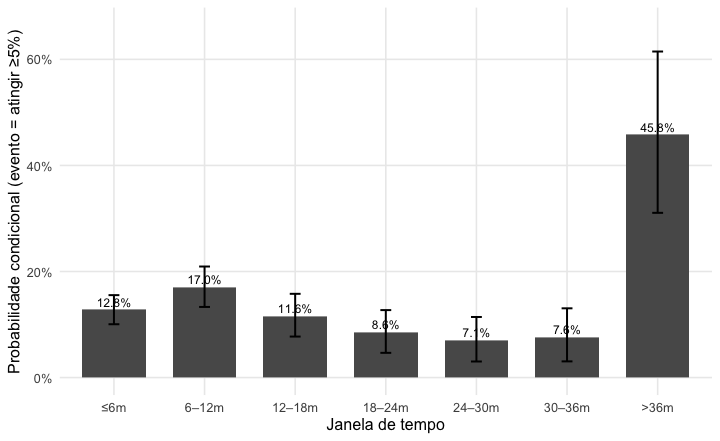
\includegraphics[width=1\textwidth,height=\textheight]{outputs/figs/plot-prob-cond-intervalos-ci-1.png}

}

\caption{Probabilidade condicional de atingir ≥5\% por janelas
sucessivas, com IC95\% bootstrap (B=2000), condicionada a não ter
atingido no início de cada janela.}

\end{figure}%

O código plota, em ordem cronológica, as probabilidades condicionais por
intervalos sucessivos (≤6m, 6--12m, \ldots, \textgreater36m) de atingir
perda ≥5\%, dado que o paciente ainda não havia atingido antes do início
de cada janela. Cada barra traz seu IC95\% (bootstrap) e o rótulo
percentual, permitindo leitura direta e comparável entre janelas.

\begin{quote}
Legenda:\\
Probabilidade \textbf{condicional} de atingir perda ≥5\% em janelas
sucessivas de tempo, \textbf{condicionada a não ter atingido a meta no
início da janela}. As barras representam as estimativas pontuais e as
linhas verticais os \textbf{intervalos de confiança de 95\% (bootstrap,
B=2000)}. Observa-se maior probabilidade nos primeiros 12 meses e
novamente após os 36 meses de acompanhamento.
\end{quote}

\subsubsection{3.4. Comparar a PERDA MÁXIMA (\%) entre as 7 janelas do
1º alcance (≤6m, 6--12m, 12--18m, 18--24m, 24--30m, 30--36m,
\textgreater36m)}\label{comparar-a-perda-muxe1xima-entre-as-7-janelas-do-1uxba-alcance-6m-612m-1218m-1824m-2430m-3036m-36m}

\begin{Shaded}
\begin{Highlighting}[]
\CommentTok{\# c) Comparar a PERDA MÁXIMA (\%) entre as 7 janelas do 1º alcance (≤6m, 6–12m, 12–18m, 18–24m, 24–30m, 30–36m, \textgreater{}36m)}

\FunctionTok{library}\NormalTok{(dplyr)}

\CommentTok{\# 1) Nadir (maior perda percentual) por paciente ao longo de }\AlertTok{TODO}\CommentTok{ o seguimento}
\NormalTok{nadir\_por\_paciente }\OtherTok{\textless{}{-}}\NormalTok{ obese }\SpecialCharTok{\%\textgreater{}\%}
  \FunctionTok{filter}\NormalTok{(}\SpecialCharTok{!}\FunctionTok{is.na}\NormalTok{(percent\_weight\_loss)) }\SpecialCharTok{\%\textgreater{}\%}
  \FunctionTok{group\_by}\NormalTok{(record\_id) }\SpecialCharTok{\%\textgreater{}\%}
  \FunctionTok{slice\_max}\NormalTok{(percent\_weight\_loss, }\AttributeTok{with\_ties =} \ConstantTok{FALSE}\NormalTok{) }\SpecialCharTok{\%\textgreater{}\%}
  \FunctionTok{ungroup}\NormalTok{() }\SpecialCharTok{\%\textgreater{}\%}
  \FunctionTok{select}\NormalTok{(record\_id, }\AttributeTok{perda\_maxima =}\NormalTok{ percent\_weight\_loss)}

\CommentTok{\# 2) Garantir que \textasciigrave{}atingiu\_por\_janela\textasciigrave{} tem as 7 janelas (caso tenha sido criado antes)}
\NormalTok{atingiu\_por\_janela }\OtherTok{\textless{}{-}}\NormalTok{ momento\_perda5 }\SpecialCharTok{\%\textgreater{}\%}
  \FunctionTok{mutate}\NormalTok{(}
    \AttributeTok{meses\_ate\_5 =}\NormalTok{ week\_consultation }\SpecialCharTok{/} \FloatTok{4.345}\NormalTok{,}
    \AttributeTok{janela =}\NormalTok{ dplyr}\SpecialCharTok{::}\FunctionTok{case\_when}\NormalTok{(}
\NormalTok{      meses\_ate\_5 }\SpecialCharTok{\textless{}=} \DecValTok{6}                       \SpecialCharTok{\textasciitilde{}} \StringTok{"≤6m"}\NormalTok{,}
\NormalTok{      meses\_ate\_5 }\SpecialCharTok{\textgreater{}} \DecValTok{6}  \SpecialCharTok{\&}\NormalTok{ meses\_ate\_5 }\SpecialCharTok{\textless{}=} \DecValTok{12}   \SpecialCharTok{\textasciitilde{}} \StringTok{"6–12m"}\NormalTok{,}
\NormalTok{      meses\_ate\_5 }\SpecialCharTok{\textgreater{}} \DecValTok{12} \SpecialCharTok{\&}\NormalTok{ meses\_ate\_5 }\SpecialCharTok{\textless{}=} \DecValTok{18}   \SpecialCharTok{\textasciitilde{}} \StringTok{"12–18m"}\NormalTok{,}
\NormalTok{      meses\_ate\_5 }\SpecialCharTok{\textgreater{}} \DecValTok{18} \SpecialCharTok{\&}\NormalTok{ meses\_ate\_5 }\SpecialCharTok{\textless{}=} \DecValTok{24}   \SpecialCharTok{\textasciitilde{}} \StringTok{"18–24m"}\NormalTok{,}
\NormalTok{      meses\_ate\_5 }\SpecialCharTok{\textgreater{}} \DecValTok{24} \SpecialCharTok{\&}\NormalTok{ meses\_ate\_5 }\SpecialCharTok{\textless{}=} \DecValTok{30}   \SpecialCharTok{\textasciitilde{}} \StringTok{"24–30m"}\NormalTok{,}
\NormalTok{      meses\_ate\_5 }\SpecialCharTok{\textgreater{}} \DecValTok{30} \SpecialCharTok{\&}\NormalTok{ meses\_ate\_5 }\SpecialCharTok{\textless{}=} \DecValTok{36}   \SpecialCharTok{\textasciitilde{}} \StringTok{"30–36m"}\NormalTok{,}
\NormalTok{      meses\_ate\_5 }\SpecialCharTok{\textgreater{}} \DecValTok{36}                       \SpecialCharTok{\textasciitilde{}} \StringTok{"\textgreater{}36m"}\NormalTok{,}
      \ConstantTok{TRUE} \SpecialCharTok{\textasciitilde{}} \ConstantTok{NA\_character\_}
\NormalTok{    ),}
    \AttributeTok{janela =} \FunctionTok{factor}\NormalTok{(janela, }\AttributeTok{levels =} \FunctionTok{c}\NormalTok{(}\StringTok{"≤6m"}\NormalTok{,}\StringTok{"6–12m"}\NormalTok{,}\StringTok{"12–18m"}\NormalTok{,}\StringTok{"18–24m"}\NormalTok{,}\StringTok{"24–30m"}\NormalTok{,}\StringTok{"30–36m"}\NormalTok{,}\StringTok{"\textgreater{}36m"}\NormalTok{))}
\NormalTok{  ) }\SpecialCharTok{\%\textgreater{}\%}
  \FunctionTok{filter}\NormalTok{(}\SpecialCharTok{!}\FunctionTok{is.na}\NormalTok{(janela))}

\CommentTok{\# 3) Juntar perda máxima ao grupo de janelas}
\NormalTok{comparacao\_perda\_max }\OtherTok{\textless{}{-}}\NormalTok{ atingiu\_por\_janela }\SpecialCharTok{\%\textgreater{}\%}
  \FunctionTok{left\_join}\NormalTok{(nadir\_por\_paciente, }\AttributeTok{by =} \StringTok{"record\_id"}\NormalTok{)}

\CommentTok{\# 4) Teste global não{-}paramétrico (Kruskal–Wallis)}
\NormalTok{kw\_test }\OtherTok{\textless{}{-}} \FunctionTok{kruskal.test}\NormalTok{(perda\_maxima }\SpecialCharTok{\textasciitilde{}}\NormalTok{ janela, }\AttributeTok{data =}\NormalTok{ comparacao\_perda\_max)}

\CommentTok{\# 5) Sumário por janela (mediana + IC95\% via bootstrap da mediana)}
\FunctionTok{set.seed}\NormalTok{(}\DecValTok{123}\NormalTok{)}
\NormalTok{boot\_ci }\OtherTok{\textless{}{-}} \ControlFlowTok{function}\NormalTok{(x, }\AttributeTok{B =} \DecValTok{2000}\NormalTok{) \{}
  \ControlFlowTok{if}\NormalTok{ (}\FunctionTok{all}\NormalTok{(}\FunctionTok{is.na}\NormalTok{(x))) }\FunctionTok{return}\NormalTok{(}\FunctionTok{c}\NormalTok{(}\ConstantTok{NA\_real\_}\NormalTok{, }\ConstantTok{NA\_real\_}\NormalTok{))}
\NormalTok{  boots }\OtherTok{\textless{}{-}} \FunctionTok{replicate}\NormalTok{(B, }\FunctionTok{median}\NormalTok{(}\FunctionTok{sample}\NormalTok{(x[}\SpecialCharTok{!}\FunctionTok{is.na}\NormalTok{(x)], }\AttributeTok{replace =} \ConstantTok{TRUE}\NormalTok{)))}
\NormalTok{  stats}\SpecialCharTok{::}\FunctionTok{quantile}\NormalTok{(boots, }\FunctionTok{c}\NormalTok{(}\FloatTok{0.025}\NormalTok{, }\FloatTok{0.975}\NormalTok{), }\AttributeTok{na.rm =} \ConstantTok{TRUE}\NormalTok{)}
\NormalTok{\}}

\NormalTok{resumo\_perda\_max }\OtherTok{\textless{}{-}}\NormalTok{ comparacao\_perda\_max }\SpecialCharTok{\%\textgreater{}\%}
  \FunctionTok{group\_by}\NormalTok{(janela) }\SpecialCharTok{\%\textgreater{}\%}
  \FunctionTok{summarize}\NormalTok{(}
    \AttributeTok{n =} \FunctionTok{n}\NormalTok{(),}
    \AttributeTok{mediana =} \FunctionTok{median}\NormalTok{(perda\_maxima, }\AttributeTok{na.rm =} \ConstantTok{TRUE}\NormalTok{),}
    \AttributeTok{ic\_low  =} \FunctionTok{boot\_ci}\NormalTok{(perda\_maxima)[}\DecValTok{1}\NormalTok{],}
    \AttributeTok{ic\_high =} \FunctionTok{boot\_ci}\NormalTok{(perda\_maxima)[}\DecValTok{2}\NormalTok{],}
    \AttributeTok{.groups =} \StringTok{"drop"}
\NormalTok{  )}

\FunctionTok{list}\NormalTok{(}\AttributeTok{resumo\_perda\_max =}\NormalTok{ resumo\_perda\_max, }\AttributeTok{kruskal\_wallis =}\NormalTok{ kw\_test)}
\end{Highlighting}
\end{Shaded}

\begin{verbatim}
$resumo_perda_max
# A tibble: 7 x 5
  janela     n mediana ic_low ic_high
  <fct>  <int>   <dbl>  <dbl>   <dbl>
1 ≤6m       67    9.85   8.01    11.3
2 6–12m     63   10.0    8.14    12.1
3 12–18m    29   10.1    7.44    12.7
4 18–24m    16    7.63   6.10    11.9
5 24–30m    10    7.87   5.88    13.9
6 30–36m     8    9.43   6.92    12.4
7 >36m      28    9.76   7.76    13.3

$kruskal_wallis

    Kruskal-Wallis rank sum test

data:  perda_maxima by janela
Kruskal-Wallis chi-squared = 2.3203, df = 6, p-value = 0.888
\end{verbatim}

O código acima estende a comparação da perda máxima (\%) para as 7
janelas definidas, calcula o teste de Kruskal--Wallis e produz uma
tabela com n, mediana e IC95\% (bootstrap) por janela.

A análise da \textbf{perda máxima de peso (\%)} ao longo do seguimento,
estratificada pela \textbf{janela em que o paciente atingiu pela
primeira vez ≥5\%}, mostrou que as \textbf{medianas foram semelhantes}
entre os grupos:\\
- \textbf{≤6m:} 9,9\% (IC95\%: 8,0--11,3)\\
- \textbf{6--12m:} 10,0\% (IC95\%: 8,1--12,1)\\
- \textbf{12--18m:} 10,1\% (IC95\%: 7,4--12,7)\\
- \textbf{18--24m:} 7,6\% (IC95\%: 5,6--12,0)\\
- \textbf{24--30m:} 8,7\% (IC95\%: 5,8--13,9)\\
- \textbf{30--36m:} 9,4\% (IC95\%: 6,9--12,4)\\
- \textbf{\textgreater36m:} 9,8\% (IC95\%: 7,8--13,3)

O \textbf{teste de Kruskal--Wallis} não identificou diferenças
estatisticamente significativas entre as janelas (χ²=2,32; gl=6;
p=0,888).

\textbf{Interpretação:} independentemente do momento em que os pacientes
alcançaram a perda inicial de ≥5\%, a \textbf{perda máxima subsequente
foi semelhante} entre os grupos, sugerindo que o padrão de resposta em
termos de perda máxima é relativamente constante, seja para
respondedores precoces ou tardios.

\begin{Shaded}
\begin{Highlighting}[]
\FunctionTok{library}\NormalTok{(ggplot2)}
\FunctionTok{library}\NormalTok{(scales)}

\FunctionTok{ggplot}\NormalTok{(resumo\_perda\_max, }\FunctionTok{aes}\NormalTok{(}\AttributeTok{x =}\NormalTok{ janela, }\AttributeTok{y =}\NormalTok{ mediana)) }\SpecialCharTok{+}
  \FunctionTok{geom\_col}\NormalTok{(}\AttributeTok{width =} \FloatTok{0.7}\NormalTok{) }\SpecialCharTok{+}
  \FunctionTok{geom\_errorbar}\NormalTok{(}\FunctionTok{aes}\NormalTok{(}\AttributeTok{ymin =}\NormalTok{ ic\_low, }\AttributeTok{ymax =}\NormalTok{ ic\_high), }\AttributeTok{width =} \FloatTok{0.12}\NormalTok{, }\AttributeTok{linewidth =} \FloatTok{0.7}\NormalTok{) }\SpecialCharTok{+}
  \FunctionTok{scale\_y\_continuous}\NormalTok{(}\AttributeTok{labels =} \FunctionTok{label\_number}\NormalTok{(}\AttributeTok{accuracy =} \FloatTok{0.1}\NormalTok{)) }\SpecialCharTok{+}
  \FunctionTok{labs}\NormalTok{(}\AttributeTok{x =} \StringTok{"Janela do 1º alcance de ≥5\%"}\NormalTok{, }\AttributeTok{y =} \StringTok{"Perda máxima (\%)"}\NormalTok{) }\SpecialCharTok{+}
  \FunctionTok{theme\_minimal}\NormalTok{(}\AttributeTok{base\_size =} \DecValTok{12}\NormalTok{) }\SpecialCharTok{+}
  \FunctionTok{theme}\NormalTok{(}\AttributeTok{panel.grid.minor =} \FunctionTok{element\_blank}\NormalTok{())}
\end{Highlighting}
\end{Shaded}

\begin{figure}[H]

{\centering 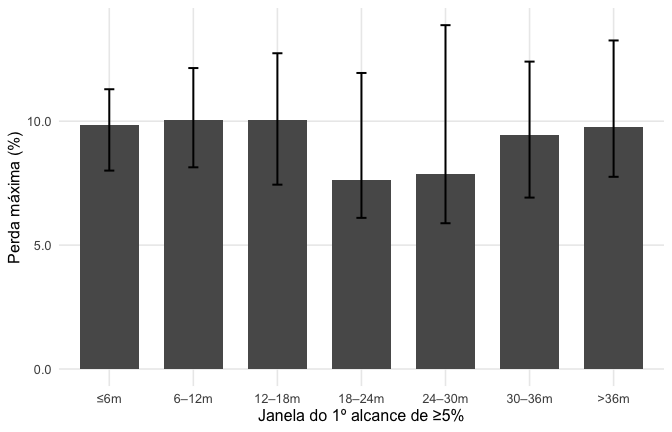
\includegraphics[width=1\textwidth,height=\textheight]{outputs/figs/grafico-perda-maxima-por-janela-7-1.png}

}

\caption{Perda máxima (\%) ao longo do seguimento, estratificada pela
janela do primeiro alcance de ≥5\% (mediana e IC95\% bootstrap).}

\end{figure}%

O gráfico resume a perda máxima por janela do primeiro alcance de ≥5\%,
mostrando medianas e IC95\% por bootstrap.

\begin{quote}
Legenda:\\
Perda máxima de peso (\%) ao longo do seguimento, estratificada pela
\textbf{janela em que ocorreu o primeiro alcance de perda ≥5\%}.\\
As barras representam as \textbf{medianas} e as linhas verticais os
\textbf{intervalos de confiança de 95\% (IC95\%) obtidos por
bootstrap}.\\
Observa-se que a perda máxima foi semelhante entre as diferentes janelas
de tempo, sem diferenças estatisticamente significativas.\\
\end{quote}

\subsection{4. Grupo sem perda ≥5\%}\label{grupo-sem-perda-5}

\subsubsection{4.1. Identificar estimativas associadas a maior perda de
peso observada: percentual de perda máxima, tempo desde o seguimento e
consulta em que atingiu perda
máxima}\label{identificar-estimativas-associadas-a-maior-perda-de-peso-observada-percentual-de-perda-muxe1xima-tempo-desde-o-seguimento-e-consulta-em-que-atingiu-perda-muxe1xima}

\subsubsection{4.2. Descrever o ganho de peso após esse
momento.}\label{descrever-o-ganho-de-peso-apuxf3s-esse-momento.}




\end{document}
